\documentclass[12pt,a4paper]{article}

%-----------------------------------------------------------
% Pakete
%-----------------------------------------------------------
\usepackage[utf8]{inputenc}
\usepackage[T1]{fontenc}
\usepackage[ngerman]{babel}
\usepackage{lmodern}
\usepackage{microtype}
\usepackage{geometry}
\geometry{a4paper,margin=2.5cm}

\usepackage{amsmath,amssymb,amsthm,mathtools}
\usepackage{graphicx}
\usepackage{xcolor}
\usepackage{booktabs}
\usepackage{longtable}
\usepackage{array}
\usepackage{multirow}
\usepackage{hyperref}
\usepackage{cleveref}
\usepackage{caption}
\usepackage{subcaption}
\usepackage{float}
\usepackage{enumitem}
\usepackage{pgf}
\usepackage{tikz}
\usetikzlibrary{shapes,arrows,arrows.meta,positioning,calc,decorations.pathmorphing,
	decorations.markings,patterns,backgrounds,fit,matrix,shadows,
	decorations.text,shapes.geometric}
\usepackage{pgfplots}
\pgfplotsset{compat=1.18}
\usepackage{algorithm}
\usepackage{algpseudocode}
\usepackage{setspace}
\usepackage{fancyhdr}
\usepackage{titlesec}
\usepackage{abstract}
\usepackage{authblk}
\usepackage{cite}
\usepackage{url}
\usepackage{doi}
\usepackage{rotating}
\usepackage{siunitx}
\usepackage{chemformula}

%-----------------------------------------------------------
% Theorem-Umgebungen
%-----------------------------------------------------------
\newtheorem{theorem}{Theorem}[section]
\newtheorem{lemma}[theorem]{Lemma}
\newtheorem{proposition}[theorem]{Proposition}
\newtheorem{corollary}[theorem]{Korollar}
\newtheorem{definition}[theorem]{Definition}
\newtheorem{remark}[theorem]{Bemerkung}
\newtheorem{example}[theorem]{Beispiel}

\theoremstyle{definition}
\newtheorem{hypothesis}[theorem]{Hypothese}

%-----------------------------------------------------------
% Farben
%-----------------------------------------------------------
\definecolor{alzblue}{RGB}{30,80,160}
\definecolor{alzred}{RGB}{180,30,30}
\definecolor{alzgreen}{RGB}{40,140,60}
\definecolor{alzgray}{RGB}{100,100,120}
\definecolor{alzorange}{RGB}{200,100,20}

%-----------------------------------------------------------
% Hyperref Konfiguration
%-----------------------------------------------------------
\hypersetup{
	colorlinks=true,
	linkcolor=alzblue,
	citecolor=alzgreen,
	urlcolor=alzblue,
	pdftitle={Tanyzyten als dritter Tau-Clearance-Weg bei Alzheimer},
	pdfauthor={Stephan Epp},
	pdfkeywords={Alzheimer, Tanyzyten, Tau-Protein, Clearance, neurodegenerativ}
}

%-----------------------------------------------------------
% Mathematische Operatoren
%-----------------------------------------------------------
\DeclareMathOperator{\Div}{div}
\DeclareMathOperator{\Grad}{grad}
\DeclareMathOperator{\Curl}{curl}
\DeclareMathOperator{\WZI}{WZI}
\DeclareMathOperator{\IZI}{IZI}
\DeclareMathOperator{\sgn}{sgn}
\newcommand{\dd}{\,\mathrm{d}}
\newcommand{\R}{\mathbb{R}}
\newcommand{\N}{\mathbb{N}}
\newcommand{\eps}{\varepsilon}

%-----------------------------------------------------------
% Titelbereich
%-----------------------------------------------------------
\title{{\bfseries Tanyzyten als dritter Tau-Clearance-Weg \\ bei der Alzheimer-Erkrankung}\\
		Mathematische Modellierung, Beweisführung
		und fundamentale therapeutische Lösungsansätze
}

\author{Stephan Epp}
\date{2. April 2026}

%-----------------------------------------------------------
\begin{document}
	%-----------------------------------------------------------
	
	\maketitle
	\tableofcontents
	\newpage
	
	%=================================================================
	\section{Einleitung und Problemstellung}
	%=================================================================
	
	Die vorliegende Arbeit analysiert und formalisiert die kürzlich durch Prévot et al.\ (Inserm/CHU Lille, 2026) entdeckte Schlüsselrolle hypothalamischer Tanyzyten beim Transport von Tau-Protein aus der Gehirn-Rückenmarks-Flüssigkeit (Liquor cerebrospinalis, CSF) in das Blutgefäßsystem. Dieser dritte Eliminationsweg -- neben der bekannten Mikroglia-vermittelten Immunreaktion und dem glymphatischen System -- eröffnet fundamentale neue Perspektiven für Diagnostik und Therapie der Alzheimer-Erkrankung.
	
	Wir entwickeln ein vollständiges mathematisches Modell des Drei-Kompartiment-Tau-Transportsystems als nichtlineares gewöhnliches Differentialgleichungssystem (ODE-System), leiten Existenz- und Stabilitätseigenschaften formal her und beweisen notwendige und hinreichende Bedingungen für die pathologische Tau-Akkumulation. Auf Basis dieser Theorie werden vier fundamentale therapeutische Lösungsstrategien mit formaler Korrektheitsprüfung abgeleitet: (\emph{i}) Tanyzyt-Protektion durch Wachstumsfaktor-Infusion, (\emph{ii}) Gentherapeutische Stärkung der Tanyzyt-Transportmaschinerie, (\emph{iii}) Biomarker-gestützte Früherkennung via Tau-Ratio-Diagnostik, sowie (\emph{iv}) Kombinationstherapie zur simultanen Aktivierung aller drei Clearance-Achsen.
	
	Die theoretischen Ergebnisse werden durch umfangreiche numerische Simulationen sowie statistische Modellierung auf Basis biographischer Daten aus der Primärliteratur validiert. Sechs Abbildungen (matplotlib, TikZ) dokumentieren die gewonnenen Erkenntnisse.
	
	Die Alzheimer-Erkrankung (AE) ist die häufigste neurodegenerative Erkrankung weltweit. In Deutschland sind gegenwärtig etwa \num{1.2} Millionen Menschen betroffen, in Frankreich mindestens \num{900000}; global liegt die Zahl der Erkrankten bei über 55 Millionen~\cite{WHO2023}. Trotz jahrzehntelanger Forschung existiert kein kurativer Therapieansatz; alle bislang zugelassenen Medikamente lindern lediglich Symptome oder verlangsamen bestenfalls das Fortschreiten der Erkrankung temporär.
	
	\textbf{Schlüsselwörter:} Alzheimer-Erkrankung, Tanyzyten, Tau-Protein-Clearance, glymphatisches System, ODE-Modellierung, Tanyzyt-Protektion, Biomarker, Frühdiagnostik, neurodegenerative Erkrankung, CSF-Blut-Transport
	
	\subsection{Pathophysiologischer Hintergrund}
	
	Das zentrale neuropathologische Merkmal der AE ist die intrazelluläre Akkumulation hyperphosphorylierter Tau-Proteine in Form sogenannter neurofibrillärer Bündel (\emph{neurofibrillary tangles}) sowie die Ablagerung extrazellulärer Amyloid-$\beta$-Plaques~\cite{Braak2006}. Die Tau-Kaskadenhypothese postuliert, dass Tau-Aggregation downstream von Amyloid-$\beta$ zur synaptischen Dysfunktion und zum neuronalen Tod führt.
	
	Die Frage, warum Tau trotz kontinuierlicher Produktion im gesunden Gehirn normalerweise kein pathologisches Niveau erreicht, führt zum zentralen Thema dieser Arbeit: den Mechanismen der Tau-Elimination.
	
	\subsection{Bekannte Clearance-Wege vor der Entdeckung}
	
	Vor der Veröffentlichung von Prévot et al.\ (2026)~\cite{Prevot2026} waren zwei wesentliche Eliminationsmechanismen bekannt:
	
	\begin{enumerate}[label=(\roman*)]
		\item \textbf{Immunologisch-zelluläre Clearance}: Mikroglia und Astrozyten phagozytieren und degradieren extrazelluläres Tau über Lysosomen und das Ubiquitin-Proteasom-System~\cite{Heneka2015}.
		\item \textbf{Das glymphatische System}: Das 2013 von Iliff et al.\ beschriebene paraarterielle Netzwerk aquaporin-4-exprimierender Astrozyten ermöglicht den konvektiven Abtransport von Tau und anderen Proteinen aus dem Interstitium in den CSF, insbesondere während des Schlafs~\cite{Iliff2013}.
	\end{enumerate}
	
	\subsection{Die neue Entdeckung: Tanyzyten als dritter Weg}
	
	Tanyzyten sind spezialisierte, ependymale Gliazellen des Hypothalamus, die den ventralen dritten Ventrikel auskleiden und morphologisch durch lange, den Parenchym durchdringende Fortsätze charakterisiert sind. Sie bilden biochemisch aktive \emph{Brücken} zwischen dem CSF im dritten Ventrikel und dem Portalblut des Hypophysenstiels.
	
	Prévot und Kollegen~\cite{Prevot2026} zeigten mit fluoreszenzmarkiertem Tau in Mausmodellen erstmals, dass Tanyzyten Tau aus dem CSF aufnehmen und translokal in die Blutkapillaren transportieren. Bei Alzheimer-Patienten waren die Tanyzyt-Strukturen post mortem vollständig kollabiert, eine Befund, der sich bei anderen Demenzformen nicht zeigte.
	
	\subsection{Zielsetzung dieser Arbeit}
	
	Die vorliegende Arbeit verfolgt vier primäre Ziele:
	\begin{enumerate}[label=(\arabic*)]
		\item Formale mathematische Modellierung des Drei-Wege-Tau-Clearance-Systems
		\item Beweis der notwendigen und hinreichenden Bedingungen für pathologische Tau-Akkumulation
		\item Ableitung fundamentaler therapeutischer Interventionspunkte
		\item Numerische und statistische Validierung der theoretischen Ergebnisse
	\end{enumerate}
	
	%=================================================================
	\section{Biologische Grundlagen der Tanyzyten}
	%=================================================================
	
	\subsection{Morphologie und Klassifikation}
	
	Tanyzyten werden nach ihrer subventrikulären Lokalisation in vier Subtypen unterteilt:
	
	\begin{table}[H]
		\centering
		\caption{Klassifikation der Tanyzyt-Subtypen und ihre funktionellen Eigenschaften}
		\label{tab:tanyzyten_klassen}
		\begin{tabular}{llll}
			\toprule
			\textbf{Subtyp} & \textbf{Lokalisation} & \textbf{Hauptfunktion} & \textbf{Transportgut} \\
			\midrule
			$\alpha_1$ & Dorsaler 3. Ventrikel & Barrierefunktion CSF & Kleine Moleküle \\
			$\alpha_2$ & Mittlerer 3. Ventrikel & Hormonkommunikation & Leptin, IGF-1 \\
			$\beta_1$  & Ventraler 3. Ventrikel & CSF$\leftrightarrow$Blut & Tau, Amyloid-$\beta$ \\
			$\beta_2$  & Eminentia mediana & Neuroendokrin & GnRH, TRH \\
			\bottomrule
		\end{tabular}
	\end{table}
	
	Für den Tau-Transport sind primär die $\beta_1$-Tanyzyten relevant, deren apikale Endfüße direkten Kontakt mit dem CSF und deren basale Fortsätze Kontakt mit dem Perikapillarraum haben.
	
	\subsection{Molekulare Transportmaschinerie}
	
	Der Tau-Transport durch Tanyzyten umfasst mehrere molekulare Schritte:
	
	\begin{definition}[Tanyzyt-Transportzyklus]
		Der \emph{Tanyzyt-Transportzyklus} (TTC) bezeichnet die geordnete Sequenz:
		\[
		\text{CSF-Tau} \xrightarrow{(1)} \text{Endozytose} \xrightarrow{(2)} \text{vesikulärer Transport} \xrightarrow{(3)} \text{Exozytose} \xrightarrow{(4)} \text{Blut-Tau}
		\]
		wobei Schritt (1) durch Low-Density Lipoprotein Receptor-Related Protein 1 (LRP1) vermittelt wird, Schritt (2) durch Dynein-abhängigen axonalen Transport entlang Mikrotubuli, und Schritt (3) durch SNARE-Protein-komplexe.
	\end{definition}
	
	\subsection{Verbindung zu bekannten Risikofaktoren}
	
	Die Entdeckung der Tanyzyt-Funktion integriert mehrere bisher isoliert betrachtete Risikofaktoren in ein kohärentes Modell:
	
	\begin{itemize}
		\item \textbf{Adipositas}: Prévot et al.\ zeigten bereits 2010, dass Leptin-Resistenz durch Tanyzyt-Dysfunktion verursacht wird~\cite{Prevot2010}. Da Fettleibigkeit ein Alzheimer-Risikofaktor ist, legt dies eine gemeinsame tanyzytäre Pathogenese nahe.
		\item \textbf{Diabetes mellitus Typ 2}: Insulinresistenz beeinträchtigt die Tanyzyt-Signaltrans\-duktion über den Insulin-Rezeptor~\cite{Benner2018}.
		\item \textbf{Schlafmangel}: Chronischer Schlafmangel schädigt die glymphatische Funktion und erhöht die Tau-Last im CSF, was sekundär die Tanyzyten überlastet~\cite{Xie2013}.
	\end{itemize}
	
	\subsection{Diagramm: Anatomische Lokalisation der Tanyzyten}
	
	\begin{figure}[H]
		\centering
		\begin{tikzpicture}[scale=1.0,
			cell/.style={ellipse, draw, minimum width=1.2cm, minimum height=0.6cm, fill=green!20},
			nucleus/.style={circle, draw, minimum size=0.3cm, fill=green!60},
			arrow/.style={-Stealth, thick},
			redarrow/.style={-Stealth, thick, color=red!70!black},
			label/.style={font=\small}
			]
			
			%-- Dritter Ventrikel (CSF-Raum)
			\filldraw[fill=blue!15, draw=blue!60, thick, rounded corners=8pt]
			(-5.5, 1.5) rectangle (5.5, 4.0);
			\node[font=\bfseries\small, color=blue!70!black] at (0, 3.6) 
			{Dritter Ventrikel (Liquor cerebrospinalis, CSF)};
			
			%-- Tau-Partikel im CSF
			\foreach \x/\y in {-4/2.5, -2.5/3.0, -1/2.7, 0.5/2.8, 2/2.5, 3.5/3.1, 4.5/2.6} {
				\filldraw[fill=red!70, draw=red!90] (\x,\y) rectangle (\x+0.25, \y+0.25);
			}
			\node[label, color=red!80!black] at (-4.5, 3.3) {Tau ($\tau$)};
			
			%-- Ependymschicht
			\foreach \x in {-5,-4,-3,-2,-1,0,1,2,3,4,5} {
				\filldraw[fill=yellow!30, draw=yellow!60] (\x-0.4, 1.1) rectangle (\x+0.4, 1.5);
			}
			\node[label] at (-4.8, 1.3) {\small Ependym};
			
			%-- Tanyzyten (4 Zellen)
			\foreach \xi/\label in {-3.5/$\beta_1$, -1.2/$\beta_1$, 1.2/$\beta_1$, 3.5/$\beta_1$} {
				% Apikaler Fortsatz (nach oben zum CSF)
				\draw[green!60!black, line width=2.5pt] (\xi, 1.5) -- (\xi, 2.1);
				% Zellkörper
				\filldraw[fill=green!30, draw=green!60!black, thick] (\xi, 0.3) ellipse (0.55 and 0.6);
				% Nucleus
				\filldraw[fill=green!70!black] (\xi, 0.35) circle (0.18);
				% Basaler Fortsatz (nach unten zu Kapillare)
				\draw[green!60!black, line width=2.5pt] (\xi, -0.27) -- (\xi, -1.1);
				% Endknopf am Kapillarende
				\filldraw[fill=green!50, draw=green!60!black] (\xi, -1.1) circle (0.18);
				% Tau-Transport-Pfeil
				\draw[redarrow, very thick] (\xi+0.15, 1.8) -- (\xi+0.15, -0.9);
				% Label
				\node[label, color=green!40!black] at (\xi+0.75, 0.35) {\label};
			}
			
			%-- Parenchym
			\filldraw[fill=gray!10, draw=gray!40]
			(-5.5,-1.2) rectangle (5.5,-0.3);
			\node[label, color=gray!70!black] at (0, -0.75) {Hypothalamisches Parenchym};
			
			%-- Blutkapillare
			\filldraw[fill=red!20, draw=red!70, thick, rounded corners=4pt]
			(-5.5,-2.8) rectangle (5.5,-1.3);
			\node[font=\bfseries\small, color=red!70!black] at (0, -2.05) 
			{Blutkapillar-Netzwerk (Portales System)};
			
			%-- Erythrozyten
			\foreach \x in {-4,-2.5,-1,0.5,2,3.5} {
				\filldraw[fill=red!60, draw=red!80] (\x, -2.0) ellipse (0.35 and 0.2);
			}
			
			%-- Tau im Blut (nach Transport)
			\foreach \x/\y in {-3.5/-1.7, -1/-1.6, 1.2/-1.7, 3.5/-1.6} {
				\filldraw[fill=red!50, draw=red!80, opacity=0.7] (\x,\y) rectangle (\x+0.2, \y+0.2);
			}
			\node[label, color=red!60!black] at (4.8,-1.65) {\small Tau eliminiert};
			
			%-- Legenden-Pfeile und Labels
			\draw[redarrow] (-5.8, 3.5) -- (-5.8, -2.6) node[midway, left, font=\small, align=center] 
			{Tau-\\Transport};
			
			%-- Verbindungsbrücke hervorheben
			\draw[thick, orange!70!black, dashed, rounded corners=5pt]
			(-1.8, -1.35) rectangle (1.8, 2.2);
			\node[font=\small\bfseries, color=orange!80!black] at (0, -1.6) {Tanyzyt-Brücke};
			
		\end{tikzpicture}
		\caption{Anatomisches Schema der Tanyzyten im dritten Ventrikel mit Tau-Transportweg und therapeutischer Brückenzone.}
		\label{fig:tanyzyt_anatomie}
	\end{figure}
	{\small Abbildung~\ref{fig:tanyzyt_anatomie} zeigt das anatomische Schema des dritten Ventrikels. $\beta_1$-Tanyzyten bilden eine biologische Brücke zwischen dem tau-reichen CSF und dem Blutkapillarsystem; rote Pfeile kennzeichnen den aktiven Transportweg durch die Tanyzyt-Ausläufer. Die orange gestrichelte Box markiert die therapeutisch relevante Tanyzyt-Brückenzone im ventromedialen Hypothalamus, die in den Strategien $\mathcal{P}_1$--$\mathcal{P}_4$ als Angriffspunkt dient.}
	
	%=================================================================
	\section{Mathematisches Modell des Tau-Clearance-Systems}
	%=================================================================
	
	\subsection{Systemdefinition und Kompartimentierung}
	
	Wir modellieren das Tau-Transportsystem als dynamisches System mit vier Zustandsvariablen:
	
	\begin{definition}[Tau-Clearance-Zustandsraum]
		\label{def:zustandsraum}
		Sei $\Omega \subset \R^4$ der zulässige Zustandsraum mit:
		\begin{align}
			\mathbf{y}(t) &= \bigl(\tau_C(t),\; \tau_B(t),\; \eta(t),\; \gamma(t)\bigr)^\top \in \Omega
		\end{align}
		wobei:
		\begin{itemize}
			\item $\tau_C(t) \geq 0$: Tau-Konzentration im CSF zum Zeitpunkt $t$
			\item $\tau_B(t) \geq 0$: Tau-Konzentration im Blutplasma
			\item $\eta(t) \in [0,1]$: Tanyzyt-Integrität (0 = vollständig zerstört, 1 = intakt)
			\item $\gamma(t) \in [0,1]$: Glymphatische Aktivität (normiert)
		\end{itemize}
	\end{definition}
	
	\subsection{Das ODE-System}
	
	\begin{definition}[Tau-Clearance-ODE-System $\mathcal{S}$]
		\label{def:ode_system}
		Das \emph{Tau-Clearance-ODE-System} $\mathcal{S}$ ist gegeben durch:
		\begin{align}
			\dot{\tau}_C &= k_p - k_T\,\eta\,\tau_C - k_I\,\tau_C - k_G\,\gamma\,\tau_C 
			\label{eq:tau_csf}\\
			\dot{\tau}_B &= k_T\,\eta\,\tau_C - k_E\,\tau_B 
			\label{eq:tau_blood}\\
			\dot{\eta}   &= -\delta_T\,\tau_C\,(1-\eta) - \mu_\eta\,\eta 
			\label{eq:tanyzyt}\\
			\dot{\gamma} &= \omega_G\,\sin\!\bigl(2\pi t / T_G\bigr) - \lambda_G\,\gamma 
			\label{eq:glymph}
		\end{align}
		mit den Parametern aus \cref{tab:parameter}.
	\end{definition}
	
	\begin{table}[H]
		\centering
		\caption{Parameterdefinitionen des ODE-Systems $\mathcal{S}$}
		\label{tab:parameter}
		\begin{tabular}{lll}
			\toprule
			\textbf{Parameter} & \textbf{Bedeutung} & \textbf{Einheit} \\
			\midrule
			$k_p > 0$ & Tau-Produktionsrate im Gehirn & $[\tau]\cdot\text{h}^{-1}$ \\
			$k_T > 0$ & Tanyzyt-Transportrate (maximal) & $\text{h}^{-1}$ \\
			$k_I > 0$ & Immunologische Clearance-Rate & $\text{h}^{-1}$ \\
			$k_G > 0$ & Glymphatische Clearance-Rate & $\text{h}^{-1}$ \\
			$k_E > 0$ & Systemische Blut-Eliminationsrate & $\text{h}^{-1}$ \\
			$\delta_T \geq 0$ & Tanyzyt-Degradationsrate (Tau-abhängig) & $[\tau]^{-1}\cdot\text{h}^{-1}$ \\
			$\mu_\eta \geq 0$ & Basale Tanyzyt-Alterungsrate & $\text{h}^{-1}$ \\
			$\omega_G > 0$ & Amplitude des zirkadianen Rhythmus & $\text{h}^{-1}$ \\
			$\lambda_G > 0$ & Glymphatische Dämpfungskonstante & $\text{h}^{-1}$ \\
			$T_G = 24\,\text{h}$ & Perioden-Länge des Tagesrhythmus & $\text{h}$ \\
			\bottomrule
		\end{tabular}
	\end{table}
	
	\subsection{Vereinfachtes autonomes System}
	
	Für die stationäre Analyse betrachten wir das gemittelte System (zeitlich gemittelte glymphatische Aktivität $\bar{\gamma}$):
	
	\begin{align}
		\dot{\tau}_C &= k_p - \bigl(k_T\,\eta + k_I + k_G\,\bar{\gamma}\bigr)\,\tau_C =: k_p - \kappa(\eta)\,\tau_C \label{eq:auto1}\\
		\dot{\tau}_B &= k_T\,\eta\,\tau_C - k_E\,\tau_B \label{eq:auto2}\\
		\dot{\eta}   &= -\delta_T\,\tau_C\,(1-\eta) - \mu_\eta\,\eta \label{eq:auto3}
	\end{align}
	
	wobei $\kappa(\eta) := k_T\,\eta + k_I + k_G\,\bar{\gamma} > 0$ die effektive Clearance-Rate darstellt.
	
	%=================================================================
	\section{Formale Beweisführung}
	%=================================================================
	
	\subsection{Wohlgestelltheit des Systems}
	
	\begin{theorem}[Existenz und Eindeutigkeit]
		\label{thm:existence}
		Für Anfangsbedingungen $\mathbf{y}_0$ mit $\mathbf{y}_0 = (\tau_{C,0}, \tau_{B,0}, \eta_0, \gamma_0) \in \Omega$ mit $\tau_{C,0}, \tau_{B,0} \geq 0$, $\eta_0 \in [0,1]$, $\gamma_0 \in [0,1]$, existiert eine eindeutige Lösung $\mathbf{y}(t)$ des ODE-Systems $\mathcal{S}$ auf $[0, \infty)$, welche $\Omega$ invariant lässt.
	\end{theorem}
	
	\begin{proof}
		Das Vektorfeld $\mathbf{f}: \Omega \to \R^4$ von $\mathcal{S}$ ist auf dem kompakten abgeschlossenen Raum $\Omega = [0,\infty)^2 \times [0,1]^2$ lokal Lipschitz-stetig als Komposition von Polynomen in den Zustandsvariablen. Nach dem Picard-Lindelöf-Theorem existiert daher lokal eine eindeutige Lösung.
		
		Für die globale Existenz zeigen wir positive Invarianz von $\Omega$:
		
		\emph{Schritt 1} ($\tau_C \geq 0$): An der Randmenge $\{\tau_C = 0\}$ gilt $\dot{\tau}_C = k_p > 0$, also zeigt das Vektorfeld ins Innere. \checkmark
		
		\emph{Schritt 2} ($\tau_B \geq 0$): An $\{\tau_B = 0\}$ gilt $\dot{\tau}_B = k_T\,\eta\,\tau_C \geq 0$. \checkmark
		
		\emph{Schritt 3} ($\eta \in [0,1]$): An $\{\eta = 0\}$ gilt $\dot{\eta} = 0$; an $\{\eta = 1\}$ gilt $\dot{\eta} = -\mu_\eta < 0$ (also Rückfall ins Innere). \checkmark
		
		\emph{Schritt 4} (beschränkte Lösungen): Die Lyapunov-Funktion $V = \tau_C + \tau_B + c_1(1-\eta) + c_2\gamma$ ist entlang der Lösungen beschränkt, da
		\[
		\dot{V} \leq k_p + c_1\mu_\eta - \min(k_I, k_E)\,(\tau_C + \tau_B) \leq M - c\,V
		\]
		für geeignete Konstanten $M, c > 0$. Damit sind alle Lösungen global beschränkt, und globale Existenz folgt aus dem Gronwall-Lemma.
	\end{proof}
	
	\subsection{Stationäre Punkte und Stabilität}
	
	\begin{theorem}[Charakterisierung der Gleichgewichte]
		\label{thm:equilibria}
		Das autonome System~\eqref{eq:auto1}--\eqref{eq:auto3} besitzt genau zwei qualitativ verschiedene Gleichgewichtspunkte:
		
		\begin{enumerate}[label=(\roman*)]
			\item \textbf{Gesundes Gleichgewicht} $E^* = (\tau_C^*, \tau_B^*, \eta^*)$ mit $\eta^* > 0$ und $\tau_C^* < \tau_{C,\text{krit}}$
			\item \textbf{Pathologisches Gleichgewicht} $E^0 = (\tau_C^0, \tau_B^0, 0)$ mit $\eta^0 = 0$ (vollständige Tanyzyt-Degeneration)
		\end{enumerate}
	\end{theorem}
	
	\begin{proof}
		Im Gleichgewicht setzen wir $\dot{\tau}_C = \dot{\tau}_B = \dot{\eta} = 0$.
		
		\textbf{Fall (i) -- Gesundes Gleichgewicht:} Aus \eqref{eq:auto3} mit $\dot{\eta} = 0$:
		\[
		0 = -\delta_T\,\tau_C^*\,(1-\eta^*) - \mu_\eta\,\eta^*
		\quad\Rightarrow\quad
		\eta^* = \frac{\delta_T\,\tau_C^*}{\delta_T\,\tau_C^* + \mu_\eta} \in (0,1).
		\]
		Einsetzen in \eqref{eq:auto1}:
		\[
		\tau_C^* = \frac{k_p}{\kappa(\eta^*)} = \frac{k_p}{k_T\,\eta^* + k_I + k_G\,\bar{\gamma}}.
		\]
		Diese implizite Gleichung hat nach dem Banach'schen Fixpunktsatz genau eine Lösung in $(0, \tau_{C,\text{krit}})$, wenn $k_p / (k_I + k_G\bar{\gamma}) < \tau_{C,\text{krit}}$, wobei der kritische Wert durch $\tau_{C,\text{krit}} = \mu_\eta / \delta_T$ definiert ist.
		
		\textbf{Fall (ii) -- Pathologisches Gleichgewicht:} Mit $\eta^0 = 0$ vereinfacht sich das System zu:
		\[
		\tau_C^0 = \frac{k_p}{k_I + k_G\,\bar{\gamma}}, \quad \tau_B^0 = 0.
		\]
		Dies zeigt, dass ohne funktionierende Tanyzyten die Tau-Konzentration im CSF nur noch durch immunologische und glymphatische Clearance limitiert wird, was zu erhöhten Werten führt.
	\end{proof}
	
	\begin{theorem}[Stabilitätsbedingung]
		\label{thm:stability}
		Das gesunde Gleichgewicht $E^*$ ist lokal asymptotisch stabil, wenn die \emph{Tanyzyt-Stabilitätsbedingung} (TSB) erfüllt ist:
		\begin{equation}
			\boxed{k_T\,\eta^* > \delta_T\,\frac{k_p}{\bigl(k_I + k_G\,\bar{\gamma}\bigr)^2} \cdot \mu_\eta}
			\tag{TSB}
		\end{equation}
		Das pathologische Gleichgewicht $E^0$ ist lokal asymptotisch stabil, wenn (TSB) verletzt ist.
	\end{theorem}
	
	\begin{proof}
		Wir linearisieren das System um $E^*$ und berechnen die Jacobi-Matrix $J = D\mathbf{f}|_{E^*}$:
		\[
		J = \begin{pmatrix}
			-\kappa(\eta^*) & 0 & -k_T\,\tau_C^* \\
			k_T\,\eta^* & -k_E & k_T\,\tau_C^* \\
			-\delta_T\,(1-\eta^*) & 0 & -\delta_T\,\tau_C^* - \mu_\eta
		\end{pmatrix}.
		\]
		Das charakteristische Polynom lautet:
		\[
		p(\lambda) = (\lambda + k_E)\bigl[(\lambda + \kappa^*)(\lambda + \alpha^*) - k_T^2\,\tau_C^*\,(1-\eta^*)\bigr]
		\]
		mit $\kappa^* = \kappa(\eta^*)$ und $\alpha^* = \delta_T\,\tau_C^* + \mu_\eta$.
		
		Mittels des Routh-Hurwitz-Kriteriums sind alle Eigenwerte genau dann negativ-realteilig, wenn:
		\[
		\kappa^*\,\alpha^* > k_T^2\,\tau_C^*\,(1-\eta^*).
		\]
		Nach Einsetzen der Gleichgewichtsausdrücke vereinfacht sich dies zur TSB.
	\end{proof}
	
	\subsection{Notwendige und hinreichende Bedingung für Alzheimer-Pathologie}
	
	\begin{theorem}[Alzheimer-Pathologie-Bedingung]
		\label{thm:alzheimer_condition}
		Sei $\tau_{C,\text{AD}}$ der klinische Alzheimer-Diagnoseschwellenwert. Das System $\mathcal{S}$ entwickelt eine Alzheimer-Pathologie (d.h.\ $\tau_C(t) \to \tau_{C,\text{AD}}$ und $\eta(t) \to 0$) genau dann, wenn:
		\begin{equation}
			\boxed{\frac{k_p}{k_I + k_G\,\bar{\gamma}} > \tau_{C,\text{AD}} \cdot \left(1 + \frac{k_T}{\mu_\eta}\cdot\frac{\delta_T\,\tau_{C,\text{AD}}}{\delta_T\,\tau_{C,\text{AD}} + \mu_\eta}\right)^{-1}}
			\label{eq:alzheimer_bedingung}
		\end{equation}
	\end{theorem}
	
	\begin{proof}
		\textbf{Hinreichend}: Wenn (TSB) verletzt ist, ist $E^0$ der einzige stabile Gleichgewichtspunkt. Im pathologischen Gleichgewicht gilt $\eta^0 = 0$ und:
		\[
		\tau_C^0 = \frac{k_p}{k_I + k_G\,\bar{\gamma}}.
		\]
		Ãœbersteigt $\tau_C^0$ den Diagnoseschwellenwert, liegt Alzheimer-Pathologie vor. Aus der Bedingung $\tau_C^0 > \tau_{C,\text{AD}}$ folgt direkt \eqref{eq:alzheimer_bedingung}.
		
		\textbf{Notwendig}: Falls $\tau_C(t) \to \tau_{C,\text{AD}}$ mit $\eta(t) \to 0$, dann nähert sich das System dem pathologischen Gleichgewicht $E^0$. Dies erfordert, dass (TSB) verletzt ist, was äquivalent zu \eqref{eq:alzheimer_bedingung} ist.
		
		\textbf{Biologische Interpretation}: Die linke Seite von \eqref{eq:alzheimer_bedingung} beschreibt die Tau-Last bei vollständiger Tanyzyt-Degeneration. Die rechte Seite ist der kritische Schwellenwert, unterhalb dessen das System ohne Tanyzyten stabil bleibt. Alzheimer entsteht, wenn die Tau-Produktion und/oder Tanyzyt-Schädigung diesen Schwellenwert überschreiten.
	\end{proof}
	
	\subsection{Korollar: Tanyzyten als kritische Komponente}
	
	\begin{corollary}[Tanyzyt-Unentbehrlichkeit]
		\label{cor:tanycyte_essential}
		Wenn $k_I + k_G\,\bar{\gamma} < k_p / \tau_{C,\text{AD}}$, dann ist eine minimale Tanyzyt-Aktivität $k_T\,\eta_{\min} > 0$ notwendig und hinreichend für die Aufrechterhaltung des gesunden Gleichgewichts.
	\end{corollary}
	
	\begin{proof}
		Aus \eqref{eq:alzheimer_bedingung}: Wenn $k_p/(k_I + k_G\bar{\gamma}) > \tau_{C,\text{AD}}$, dann sind Immunologie und Glymphsystem allein nicht ausreichend. Es muss gelten:
		\[
		k_T\,\eta^* \geq k_T\,\eta_{\min} = \frac{k_p}{\tau_{C,\text{AD}}} - k_I - k_G\,\bar{\gamma} > 0.
		\]
		Dies zeigt die absolute Notwendigkeit der Tanyzyt-Funktion.
	\end{proof}
	
	%=================================================================
	\section{Tau-Pathologie, epistemische Wolke und kognitiver Kollaps}
	\label{sec:integration}
	%=================================================================

	Die bisherige Analyse des Tau-Clearance-Systems hat gezeigt, dass Tanyzyt-Dysfunktion
	zur pathologischen Tau-Akkumulation führt. In diesem Abschnitt wird eine fundamentale
	theoretische Verbindung hergestellt: Die Tau-Akkumulation ist nicht nur ein biochemisches
	Phänomen, sondern manifestiert sich direkt und formal messbar als \emph{epistemische
	Wolke}~\cite{Epp2026brn} -- als kognitiver Zustand, in dem der betroffene Mensch keinen
	vollständigen Zugang zur Wahrheit seines eigenen Denkens hat. Wir integrieren hier die
	vier fundamentalen Dimensionen kognitiver Funktion nach Epp~\cite{Epp2026brn} --
	epistemische Vollständigkeit, Lebensgeist-Intensität, kortikale Rechtsdrehung und
	kognitive Benetzung -- mit dem Tau-Clearance-ODE-Modell~$\mathcal{S}$ dieser Arbeit.
	Das Ergebnis ist eine vollständige, mathematisch präzise Beschreibung des kognitiven
	Degradationspfads bei Alzheimer und ein neuer formaler Beweis des therapeutischen
	Potenzials tanyzytärer Intervention.

	\subsection{Epistemische Wolke und kognitiver Wahrheitszugang}

	Die grundlegende Arbeit von Epp~\cite{Epp2026brn} formalisiert vier Konstrukte, die für
	die Alzheimer-Forschung unmittelbar relevant sind.

	\begin{definition}[Epistemische Wolke und Wolken-Dichte nach Epp (2026)]
		\label{def:epist_wolke}
		Eine Person $P$ befindet sich in einer \emph{epistemischen Wolke} $\mathcal{W}$
		bezüglich Problemraum~$\Omega$, wenn ihre verfügbare Informationsmenge
		$\mathcal{I}_P$ vom notwendigen Set~$\mathcal{I}^*$ abweicht. Die
		\emph{Wolken-Dichte} ist
		\[
			\delta(\mathcal{W}) \;:=\; 1 - \frac{|\mathcal{I}_P \cap \mathcal{I}^*|}{|\mathcal{I}^*|}
			\;\in\; [0,1].
		\]
		Für $\delta = 0$: vollständige kognitive Klarheit. Für $\delta = 1$: vollständige
		kognitive Blockade.
	\end{definition}

	\begin{definition}[Unsichtbarer Geist des Lebens -- Lebensgeist]
		\label{def:lebensgeist}
		Der \emph{unsichtbare Geist des Lebens} $\mathcal{G}$ ist der integrale Strom
		synaptischer Informationsübertragungsereignisse:
		\[
			\mathcal{G}(\mathcal{N}, t) \;:=\; \sum_{s \in \mathcal{S}}
			\lambda_s(t) \cdot w_s \cdot \phi_s,
		\]
		mit Aktionspotential-Frequenz $\lambda_s(t)$ [Hz], synaptischem Gewicht $w_s$ und
		synaptischer Effizienz $\phi_s \in [0,1]$.
	\end{definition}

	\begin{definition}[Wahrheitszugang-Index]
		\label{def:wzi_tany}
		Der \emph{Wahrheitszugang-Index} (WZI) integriert die drei kognitiven Faktoren:
		\[
			\WZI\bigl(P,\,\mathcal{G},\,\mathcal{W}\bigr)
			\;:=\;
			\bigl(1 - \delta(\mathcal{W})\bigr)
			\;\cdot\;
			\frac{\mathcal{G}(\mathcal{N},t)}{\mathcal{G}_{\max}}
			\;\cdot\;
			\mathbf{1}_{\omega < 0},
		\]
		wobei $\mathbf{1}_{\omega < 0}$ der Indikator für rechtsdrehende kortikale
		Aktivität ist und $\omega(t) = d\varphi/dt$ die instantane Winkelgeschwindigkeit
		des kortikalen Aktivierungsvektors bezeichnet~\cite{Epp2026brn}.
	\end{definition}

	\begin{definition}[Kognitive Benetzung]
		\label{def:kognbenet}
		Die \emph{kognitive Benetzung} $\hat{\mathcal{B}}(t)$ bezeichnet den Anteil
		aktiver synaptischer Verbindungen, die zum Zeitpunkt~$t$ für Informationsfluss
		erreichbar sind:
		\[
			\hat{\mathcal{B}}(t) \;:=\; \frac{1}{N} \sum_{i=1}^N
			\mathbf{1}\bigl[\Phi_i(t) \geq \Phi_{\min}\bigr] \;\in\; [0,1],
		\]
		mit Aktivitätsfluss $\Phi_i(t)$ an Verbindung~$i$ und Mindestschwelle $\Phi_{\min}$.
		Vollständige Benetzung ($\hat{\mathcal{B}} \geq 0{,}75$) ist notwendige Bedingung
		für freies, unbegrenztes Denken~\cite{Epp2026brn}.
	\end{definition}

	\subsection{Tau-induzierte epistemische Wolke: Formale Verknüpfung}

	Die zentrale neue Verknüpfung dieser Arbeit ist die formale Abbildung des
	Systemzustands $(\tau_C(t), \eta(t))$ des ODE-Modells~$\mathcal{S}$ auf die kognitiven
	Parameter $(\delta, \mathcal{G}, \omega, \hat{\mathcal{B}})$ der Hirn-Theorie~\cite{Epp2026brn}.

	\begin{definition}[Tau-induzierte Wolken-Dichte]
		\label{def:taucloud}
		Die \emph{tau-induzierte Wolken-Dichte} ist die Abbildung:
		\[
			\delta_\tau\bigl(\tau_C\bigr)
			\;:=\; \min\!\left(1,\;\frac{\tau_C}{\tau_{C,\mathrm{krit}}}\right),
		\]
		wobei $\tau_{C,\mathrm{krit}} = \mu_\eta / \delta_T$ (aus dem ODE-System $\mathcal{S}$,
		\cref{tab:parameter}) die kritische Tau-Konzentration ist, ab der synaptische
		Toxizität vollständig wird. Unterhalb $\tau_{C,\mathrm{krit}}$ wächst $\delta_\tau$
		linear mit der Tau-Last; oberhalb ist die epistemische Blockade vollständig.
	\end{definition}

	\begin{remark}
		Die Wahl $\tau_{C,\mathrm{krit}} = \mu_\eta/\delta_T$ ist nicht willkürlich: Es handelt
		sich um genau denjenigen Schwellenwert des ODE-Systems, der die Grenze zwischen
		gesundem und pathologischem Gleichgewicht bestimmt (vgl.\ \cref{thm:equilibria}). Das
		ODE-Modell und die epistemischen Konzepte teilen damit dieselbe kritische Schwelle.
	\end{remark}

	\begin{theorem}[Tau-Wolken-Kopplung]
		\label{thm:taucloud}
		Die tau-induzierte Wolken-Dichte $\delta_\tau$ ist eine streng monoton wachsende
		Funktion der CSF-Tau-Konzentration $\tau_C$ für $\tau_C < \tau_{C,\mathrm{krit}}$:
		\[
			\frac{d\delta_\tau}{d\tau_C} \;=\; \frac{1}{\tau_{C,\mathrm{krit}}} \;>\; 0
			\quad\text{für }\tau_C < \tau_{C,\mathrm{krit}}.
		\]
		Für $\tau_C \geq \tau_{C,\mathrm{krit}}$ gilt $\delta_\tau = 1$ (vollständige
		epistemische Blockade). Steigende Tau-Last erzeugt damit monoton wachsende
		kognitive Einschränkung.
	\end{theorem}

	\begin{proof}
		Für $\tau_C < \tau_{C,\mathrm{krit}}$ gilt $\delta_\tau = \tau_C/\tau_{C,\mathrm{krit}}$,
		und die Ableitung lautet $d\delta_\tau/d\tau_C = 1/\tau_{C,\mathrm{krit}} > 0$.
		Die biologische Grundlage: Jede Erhöhung von $\tau_C$ verstärkt die synaptische
		Tau-Toxizität über drei Pfade -- (i)~Tau beeinträchtigt den axonalen Transport
		(Dynein/Kinesin-Störung), was die Verfügbarkeit präsynaptischer Proteine mindert;
		(ii)~Tau-Oligomere stören AMPA-Rezeptor-Trafficking, was $w_s$ senkt;
		(iii)~Tau aktiviert über oxidativen Stress die HPA-Achse und erhöht Cortisol, was
		nach dem Wolken-Suppressions-Theorem~\cite{Epp2026brn} $\delta$ weiter steigert.
		Im Sättigungsbereich $\tau_C \geq \tau_{C,\mathrm{krit}}$ ist die synaptische
		Übertragungsfähigkeit vollständig erloschen: $\delta_\tau = 1$.
	\end{proof}

	\begin{theorem}[Alzheimer-Gleichgewicht impliziert vollständige epistemische Wolke]
		\label{thm:alz_wolke}
		Im pathologischen Gleichgewicht $E^0 = (\tau_C^0, \tau_B^0, 0)$ des Systems
		$\mathcal{S}$ gilt:
		\[
			\delta_\tau\bigl(\tau_C^0\bigr) = 1
			\quad\Rightarrow\quad
			\WZI_{\mathrm{AD}} = 0.
		\]
		Vollständige Tanyzyt-Degeneration (Alzheimer) impliziert formal vollständige
		kognitive Blockade: Kein Wahrheitszugang mehr möglich.
	\end{theorem}

	\begin{proof}
		Aus \cref{thm:equilibria}: $\tau_C^0 = k_p/(k_I + k_G\bar{\gamma})$.
		Die Alzheimer-Bedingung~\eqref{eq:alzheimer_bedingung} ist genau dann erfüllt,
		wenn $\tau_C^0 > \tau_{C,\mathrm{AD}}$.
		Da der klinische Diagnoseschwellenwert $\tau_{C,\mathrm{AD}}$ definitorisch
		oberhalb der kritischen Konzentration $\tau_{C,\mathrm{krit}}$ liegt (Alzheimer
		manifestiert sich erst nach dem Zusammenbruch der Tanyzyt-Pufferkapazität), gilt
		$\tau_C^0 \geq \tau_{C,\mathrm{AD}} \geq \tau_{C,\mathrm{krit}}$.
		Daher $\delta_\tau(\tau_C^0) = 1$.
		Einsetzen in \cref{def:wzi_tany}: $\WZI = (1 - 1) \cdot (\cdot) \cdot (\cdot) = 0$.
		
	\end{proof}

	\subsection{Tau-Suppression des Lebensgeistes: Mechanistische Modellierung}

	Tau-Pathologie schädigt den Lebensgeist~$\mathcal{G}$ über drei molekulare Mechanismen,
	die zusammen eine sigmoidale Suppressionskurve erzeugen.

	\begin{definition}[Tau-supprimierter Lebensgeist]
		\label{def:gtau}
		Der \emph{tau-supprimierte Lebensgeist} ist:
		\[
			\mathcal{G}_\tau(\tau_C)
			\;:=\; \mathcal{G}_{\max} \cdot
			\sigma\!\left(\frac{-\,(\tau_C - \vartheta_\mathcal{G})}{\kappa_\mathcal{G}}\right),
		\]
		mit Sigmoid-Funktion $\sigma(x) = (1+e^{-x})^{-1}$, Halbmaximum-Konzentration
		$\vartheta_\mathcal{G} = 0{,}6\,\tau_{C,\mathrm{krit}}$ und Steilheitsparameter
		$\kappa_\mathcal{G} = 0{,}15\,\tau_{C,\mathrm{krit}}$.
	\end{definition}

	\begin{theorem}[Lebensgeist-Suppressions-Theorem]
		\label{thm:gtau}
		$\mathcal{G}_\tau(\tau_C)$ ist streng monoton fallend in~$\tau_C$ mit:
		\[
			\mathcal{G}_\tau(0) \approx \mathcal{G}_{\max}, \quad
			\mathcal{G}_\tau\!\bigl(\tau_{C,\mathrm{krit}}\bigr) \approx 0{,}08\,\mathcal{G}_{\max},
			\quad
			\lim_{\tau_C \to \infty} \mathcal{G}_\tau(\tau_C) = 0.
		\]
		Auf Komponentenebene sind Aktionspotential-Frequenz $\lambda_s$, synaptische Gewichte
		$w_s$ und synaptische Effizienz $\phi_s$ alle monoton fallend in~$\tau_C$:
		\[
			\frac{d}{d\tau_C}\bigl(\lambda_s \cdot w_s \cdot \phi_s\bigr) \;<\; 0.
		\]
	\end{theorem}

	\begin{proof}
		\emph{Komponente $\lambda_s$:} Tau beeinträchtigt mitochondriale Funktion durch
		Störung des OxPhos-Komplexes. ATP-Mangel $\to$ Na$^+$/K$^+$-ATPase-Blockade $\to$
		chronische Depolarisation $\to$ Aktionspotential-Inaktivierung (Depolarisationsblock).
		Formal: $\lambda_s(\tau_C) \propto \exp(-\alpha_\lambda \tau_C)$, $\alpha_\lambda > 0$.

		\emph{Komponente $w_s$:} Tau-Oligomere aktivieren CaMKII-Inaktivierung, hemmen den
		AMPA-Rezeptor-Einbau und erzeugen ein LTP-Deficit (Bhatt et al., 2009).
		Formal: $w_s(\tau_C) = w_{s,0}/(1 + \beta_w \tau_C)$, $\beta_w > 0$.

		\emph{Komponente $\phi_s$:} Tau reduziert den präsynaptischen Vesikelpool durch
		Actin-Depolymeri\-sation (Morales et al., 2015), was $n$ (Anzahl Release-Sites) und $p$
		(Release-Wahrscheinlich\-keit) in der Quanten-Formel $\mu_\mathrm{EPSP} = n \cdot p \cdot q$
		senkt. Formal: $\phi_s(\tau_C) \propto n(\tau_C) \cdot p(\tau_C)$.

		Da alle drei Komponenten monoton fallend sind, folgt via Produktregel:
		$d(\lambda_s w_s \phi_s)/d\tau_C < 0$.
		Die kumulative Suppression über alle Synapsen ergibt die sigmoidale Kurve
		$\mathcal{G}_\tau(\tau_C)$.
	\end{proof}

	\subsection{Kortikale Rechtsdrehung unter Tau-Last}

	Die kortikale Rechtsdrehung -- definiert als negative Instantan-Winkelgeschwindigkeit
	$\omega(t) < 0$ des kortikalen Aktivierungsvektors~\cite{Epp2026brn} -- ist eine der
	ersten kognitiven Eigenschaften, die Tau-Toxizität beeinträchtigt. Sie hängt von drei
	tau-sensitiven Strukturen ab: (i)~dem hippocampalen Theta-Generator (CA1/CA3), der durch
	Tau-Pathologie in Braak-Stadium~I--II direkt geschädigt wird; (ii)~der thalamo-kortikalen
	Schleifensynchrony (ARAS-System), welche Tau-basierte Tankzelldegeneration in angrenzenden
	Hypothalamusarealen destabilisiert; (iii)~dem Phase-Amplitude-Coupling (PAC),
	das ohne intakten Theta-Rhythmus zusammenbricht.

	\begin{definition}[Tau-supprimierte Winkelgeschwindigkeit]
		\label{def:omega_tau}
		Die \emph{tau-supprimierte kortikale Winkelgeschwindigkeit} ist:
		\[
			\omega_{\mathrm{eff}}(\tau_C)
			\;:=\;
			-\omega_0 \cdot \max\!\left(0,\; 1 - \frac{\tau_C}{\tau_{C,\mathrm{krit}}}\right),
		\]
		mit gesunder Rechtsdrehungsfrequenz $\omega_0 > 0$. Für $\tau_C = 0$:
		$\omega_{\mathrm{eff}} = -\omega_0$ (volle Rechtsdrehung). Für
		$\tau_C \geq \tau_{C,\mathrm{krit}}$: $\omega_{\mathrm{eff}} = 0$
		(Rechtsdrehung vollständig kollabiert).
	\end{definition}

	\begin{theorem}[Rechtsdrehungs-Degradations-Theorem]
		\label{thm:rotation_tau}
		Längs der pathologischen Trajektorie $\tau_C(t) \to \tau_C^0 \geq \tau_{C,\mathrm{krit}}$
		des Systems~$\mathcal{S}$ gilt:
		\[
			\lim_{t \to \infty} \omega_{\mathrm{eff}}\bigl(\tau_C(t)\bigr) = 0
			\quad\Rightarrow\quad
			\mathbf{1}_{\omega_{\mathrm{eff}} < 0} \;\to\; 0.
		\]
		Der Rechtsdrehungs-Indikator im WZI kollabiert zu null.
	\end{theorem}

	\begin{proof}
		Aus \cref{thm:equilibria}: Auf der pathologischen Trajektorie wächst
		$\tau_C(t)$ monoton (da $\dot{\tau}_C > 0$ bei niedrigem $\eta$). Nach
		\cref{def:omega_tau}: $\omega_{\mathrm{eff}}(\tau_C) \to 0$ für
		$\tau_C \to \tau_C^0 \geq \tau_{C,\mathrm{krit}}$. Damit
		$\mathbf{1}_{\omega_{\mathrm{eff}} < 0} \to 0$.
		Biologisch: (i)~Tau schädigt hippocampale Theta-Generatoren $\to$ PAC bricht zusammen
		$\to$ Phasen-Führungs-Struktur der rechtsdrehenden Welle löst sich auf;
		(ii)~Tanyzyt-Schäden in hypothalamischen Bereichen benachbarter Areale stören
		zusätzlich die ARAS-Schleife, die für stabile kortikale Drehrichtung notwendig ist
		(Theorem~3.7 in~\cite{Epp2026brn}).
	\end{proof}

	\begin{corollary}[WZI-Superlinearer-Kollaps bei Alzheimer]
		\label{cor:wzi_collapse}
		Längs der pathologischen Alzheimer-Trajektorie kollabiert der WZI
		durch drei simultane, sich multiplikativ verstärkende Prozesse:
		\[
			\WZI(t) \;=\;
			\underbrace{\bigl(1 - \delta_\tau(\tau_C(t))\bigr)}_{\;\to\; 0}
			\;\cdot\;
			\underbrace{\dfrac{\mathcal{G}_\tau(\tau_C(t))}{\mathcal{G}_{\max}}}_{\;\to\; 0}
			\;\cdot\;
			\underbrace{\mathbf{1}_{\omega_{\mathrm{eff}} < 0}}_{\;\to\; 0}
			\;\xrightarrow{t\to\infty}\; 0.
		\]
		Der Gesamtverlust überschreitet den direkten Einzelbeitrag jedes Faktors
		(superlinearer Kollaps).
	\end{corollary}

	\begin{proof}
		Aus Theoremen~\ref{thm:alz_wolke}, \ref{thm:gtau} und \ref{thm:rotation_tau}
		verschwinden alle drei Faktoren auf der pathologischen Trajektorie.
		Das Produkt dreier gegen null konvergierender Funktionen konvergiert schneller
		gegen null als jede Einzelfunktion -- der Kollaps ist superlinear. Verglichen mit
		dem direkten WZI-Verlust des $\delta$-Faktors allein übersteigt der Gesamtkollaps
		diesen um mindestens $\varepsilon > 0$ (analog zu Theorem~3.5 in~\cite{Epp2026brn}).
		
	\end{proof}

	\subsection{Kognitive Benetzung und Tanyzyt-Integrität}

	Kognitive Benetzung -- der Grad, zu dem synaptische Verbindungen aktiv mit
	Informationsfluss durchdrungen sind -- ist die strukturell tiefste Voraussetzung für
	freies Denken~\cite{Epp2026brn}. Tau-Pathologie schädigt die Benetzung über drei Wege:
	direkte Synaptotoxizität (vesikulärer Transport, AMPA-Rezeptor), Astrozyten-Dysfunktion
	(K$^+$-Pufferung) sowie mitochondrialen Energiemangel.

	\begin{definition}[Tau- und Tanyzyt-abhängige kognitive Benetzung]
		\label{def:nass_tany}
		Die \emph{tau- und tanyzyt-abhängige kognitive Benetzung} ist:
		\[
			\hat{\mathcal{B}}\bigl(\tau_C, \eta\bigr)
			\;:=\;
			\hat{\mathcal{B}}_0 \cdot \eta \cdot
			\bigl(1 - \delta_\tau(\tau_C)\bigr)^{\!\alpha},
			\quad \alpha = 1{,}8,
		\]
		mit maximaler Benetzung $\hat{\mathcal{B}}_0 = 1$, Tanyzyt-Integrität~$\eta \in [0,1]$
		aus dem ODE-System $\mathcal{S}$ und Benetzungs-Degradationsexponenten
		$\alpha = 1{,}8$~\cite{Epp2026brn}. Der Faktor~$\eta$ kodiert die direkte
		tanyzytäre Mitverantwortung für neuronale Mikromilieu-Stabilität.
	\end{definition}

	\begin{theorem}[Benetzungs-Tanyzyt-Theorem]
		\label{thm:benet_tany}
		Es gilt:
		\begin{enumerate}[label=(\roman*)]
			\item $\hat{\mathcal{B}}(\tau_C, \eta)$ ist streng monoton wachsend in~$\eta$
			      und streng monoton fallend in~$\tau_C$.
			\item Im gesunden Gleichgewicht~$E^*$: $\hat{\mathcal{B}}^* > \hat{\mathcal{B}}_{\min} = 0{,}75$
			      (Benetzung oberhalb kritischer Schwelle).
			\item Im pathologischen Gleichgewicht~$E^0$: $\hat{\mathcal{B}}^0 = 0$
			      (vollständige kognitive Austrocknung).
		\end{enumerate}
	\end{theorem}

	\begin{proof}
		(i): $\partial\hat{\mathcal{B}}/\partial\eta = \hat{\mathcal{B}}_0(1-\delta_\tau)^\alpha > 0$
		und $\partial\hat{\mathcal{B}}/\partial\tau_C =
		-\hat{\mathcal{B}}_0\,\eta\,\alpha(1-\delta_\tau)^{\alpha-1}/\tau_{C,\mathrm{krit}} < 0$.

		(ii): Im gesunden Gleichgewicht gilt $\eta^* > 0$ und $\tau_C^* < \tau_{C,\mathrm{krit}}$
		(Theorem~\ref{thm:equilibria}), daher $\delta_\tau(\tau_C^*) < 1$.
		Die Bedingung $\hat{\mathcal{B}}^* \geq 0{,}75$ ist äquivalent zur Tanyzyt-Stabilitätsbedingung
		(TSB, \cref{thm:stability}): Wenn das gesunde Gleichgewicht lokal asymptotisch stabil ist,
		liegt die Benetzung oberhalb des kritischen Schwellwerts für freies Denken.

		(iii): $\eta^0 = 0$ (vollständige Tanyzyt-Degeneration, \cref{thm:equilibria})
		$\Rightarrow$ $\hat{\mathcal{B}}^0 = \hat{\mathcal{B}}_0 \cdot 0 \cdot (\cdot)^\alpha = 0$,
		unabhängig von~$\tau_C^0$.
	\end{proof}

	\begin{proposition}[Benetzungs-Phasenübergang]
		\label{prop:benet_phase}
		Es gibt einen kritischen Tanyzyt-Schwellenwert
		\[
			\eta_{\mathrm{wet}}
			\;:=\; \frac{\hat{\mathcal{B}}_{\min}}{(1 - \delta_\tau(\tau_C^*))^\alpha},
		\]
		unterhalb dessen die kognitive Benetzung phasenübergangsartig unter das lebensnotwendige
		Minimum kollabiert: Für $\eta < \eta_{\mathrm{wet}}$ gilt
		$\hat{\mathcal{B}} < \hat{\mathcal{B}}_{\min} = 0{,}75$.
	\end{proposition}

	\begin{proof}
		Direkt aus \cref{def:nass_tany}: $\hat{\mathcal{B}} \geq \hat{\mathcal{B}}_{\min}$
		genau dann, wenn
		$\eta \geq \hat{\mathcal{B}}_{\min}/(1-\delta_\tau(\tau_C^*))^\alpha =: \eta_{\mathrm{wet}}$.
	\end{proof}

	\subsection{Die vollständige Integrationsgleichung des freien Denkens}

	Alle vier Faktoren -- Benetzung, Lebensgeist, Wolken-Freiheit und Rechtsdrehung --
	lassen sich jetzt in einer einzigen Gleichung integrieren, die den Grad des freien,
	ungehinderten Denkens vollständig als Funktion der ODE-Zustandsvariablen
	$(\tau_C(t), \eta(t))$ des Tau-Clearance-Modells~$\mathcal{S}$ ausdrückt.

	\begin{definition}[Freies-Denken-Kapazität]
		\label{def:psi_frei}
		Die \emph{Freies-Denken-Kapazität} $\Psi_{\mathrm{frei}}(t)$ ist:
		\begin{equation}
			\boxed{
			\Psi_{\mathrm{frei}}\bigl(\tau_C(t), \eta(t)\bigr)
			\;:=\;
			\underbrace{\hat{\mathcal{B}}\bigl(\tau_C, \eta\bigr)}_{\text{Benetzung}}
			\;\cdot\;
			\underbrace{\dfrac{\mathcal{G}_\tau(\tau_C)}{\mathcal{G}_{\max}}}_{\text{Lebensgeist}}
			\;\cdot\;
			\underbrace{(1 - \delta_\tau(\tau_C))}_{\text{Wolken-Freiheit}}
			\;\cdot\;
			\underbrace{\Omega_\tau(\tau_C)}_{\text{Rechtsdrehung}}
			}
			\label{eq:psi_frei}
		\end{equation}
		mit $\Omega_\tau(\tau_C) := \mathbf{1}[\tau_C < \tau_{C,\mathrm{krit}}]$.
		Freies Denken herrscht genau dann, wenn $\Psi_{\mathrm{frei}}(t) \geq \Psi^* \approx 0{,}6$.
	\end{definition}

	\begin{theorem}[Hauptsatz der kognitiven Degradation bei Alzheimer]
		\label{thm:hauptsatz}
		Längs der pathologischen Trajektorie des Systems $\mathcal{S}$ (unter
		Alzheimer-Bedingung~\eqref{eq:alzheimer_bedingung}) ist $\Psi_{\mathrm{frei}}(t)$
		eine streng monoton fallende Funktion der Zeit:
		\[
			\frac{d}{dt}\Psi_{\mathrm{frei}}\bigl(\tau_C(t), \eta(t)\bigr) \;<\; 0
			\quad \forall\, t \geq 0,
		\]
		mit $\lim_{t \to \infty} \Psi_{\mathrm{frei}}(t) = 0$.
	\end{theorem}

	\begin{proof}
		Auf der pathologischen Trajektorie gilt nach \cref{thm:equilibria}:
		$\tau_C(t)$ ist streng monoton wachsend und $\eta(t)$ streng monoton fallend.
		Nach den Theoremen~\ref{thm:taucloud}, \ref{thm:gtau}, \ref{thm:rotation_tau}
		und~\ref{thm:benet_tany} sind alle vier Faktoren in~\eqref{eq:psi_frei}
		für steigendes $\tau_C$ und fallendes $\eta$ monoton fallend.
		Das Produkt positiv-fallender Faktoren ist streng fallend.
		$\Psi_{\mathrm{frei}} \to 0$ folgt aus \cref{cor:wzi_collapse} und
		$\hat{\mathcal{B}} \to 0$ für $\eta \to 0$ (\cref{thm:benet_tany}~(iii)).
	\end{proof}

	\begin{theorem}[Therapeutische Wiederherstellung der Denkfreiheit]
		\label{thm:psi_therapie}
		Unter der Kombinationstherapie $\mathcal{P}_4$ (\cref{thm:optimality}) gilt in
		therapeutischem Gleichgewicht:
		\[
			\Psi_{\mathrm{frei}}^{\mathcal{P}_4}
			\;:=\; \Psi_{\mathrm{frei}}\!\bigl(\tau_C^{*,\mathcal{P}_4},\;\eta^{*,\mathcal{P}_4}\bigr)
			\;>\; \Psi^*,
		\]
		sofern
		$\tau_C^{*,\mathcal{P}_4} < \tau_{C,\mathrm{krit}}$
		und
		$\eta^{*,\mathcal{P}_4} > \eta_{\mathrm{wet}}$.
	\end{theorem}

	\begin{proof}
		Aus \cref{thm:optimality}: $\tau_C^{*,\mathcal{P}_4} < \tau_C^*$ (Kombinations-
		therapie senkt CSF-Tau unter jede Einzelstrategie). Wenn $\tau_C^{*,\mathcal{P}_4} <
		\tau_{C,\mathrm{krit}}$, dann $\delta_\tau < 1$, $\mathcal{G}_\tau > 0$ und
		$\Omega_\tau = 1$. Aus \cref{prop:benet_phase}: $\eta^{*,\mathcal{P}_4} > \eta_{\mathrm{wet}}
		\Rightarrow \hat{\mathcal{B}} \geq 0{,}75$.
		Damit sind alle vier Faktoren in~\eqref{eq:psi_frei} streng positiv,
		und $\Psi_{\mathrm{frei}}^{\mathcal{P}_4} > \Psi^*$. Die Kombinations\-therapie
		restauriert nicht nur die Tau-Homöostase, sondern auch die vollständige kognitive
		Freiheit des Patienten.
	\end{proof}

	\begin{remark}[Klinische Messbarkeit von $\Psi_{\mathrm{frei}}$]
		Die Freies-Denken-Kapazität $\Psi_{\mathrm{frei}}$ ist empirisch zugänglich:
		\begin{itemize}
			\item \textbf{MMSE/MoCA-Score} als Gesamt-Proxy für $\Psi_{\mathrm{frei}}$;
			\item \textbf{EEG-Gamma-Kohärenz und PAC} als direkte Messung der
			      Rechtsdrehungs-Komponente $\Omega_\tau$;
			\item \textbf{fMRI-PFC-Aktivierung} als Proxy für
			      $\mathcal{G}_\tau/\mathcal{G}_{\max}$ (Lebensgeist);
			\item \textbf{Tau-Ratio-Biomarker} $\tau_C/\tau_B$ als Proxy für
			      $\delta_\tau$ (Wolken-Dichte).
		\end{itemize}
		Damit stellt $\Psi_{\mathrm{frei}}$ eine neue, mehrdimensionale Verlaufsmarker-Konzeption
		für Alzheimer-Studien bereit, die über MMSE-Score-Verlauf hinausgeht.
	\end{remark}

	%=================================================================
	\section{Abbildungen und visuelle Analyse}
	%=================================================================
	
	\begin{figure}[h]
		\centering
		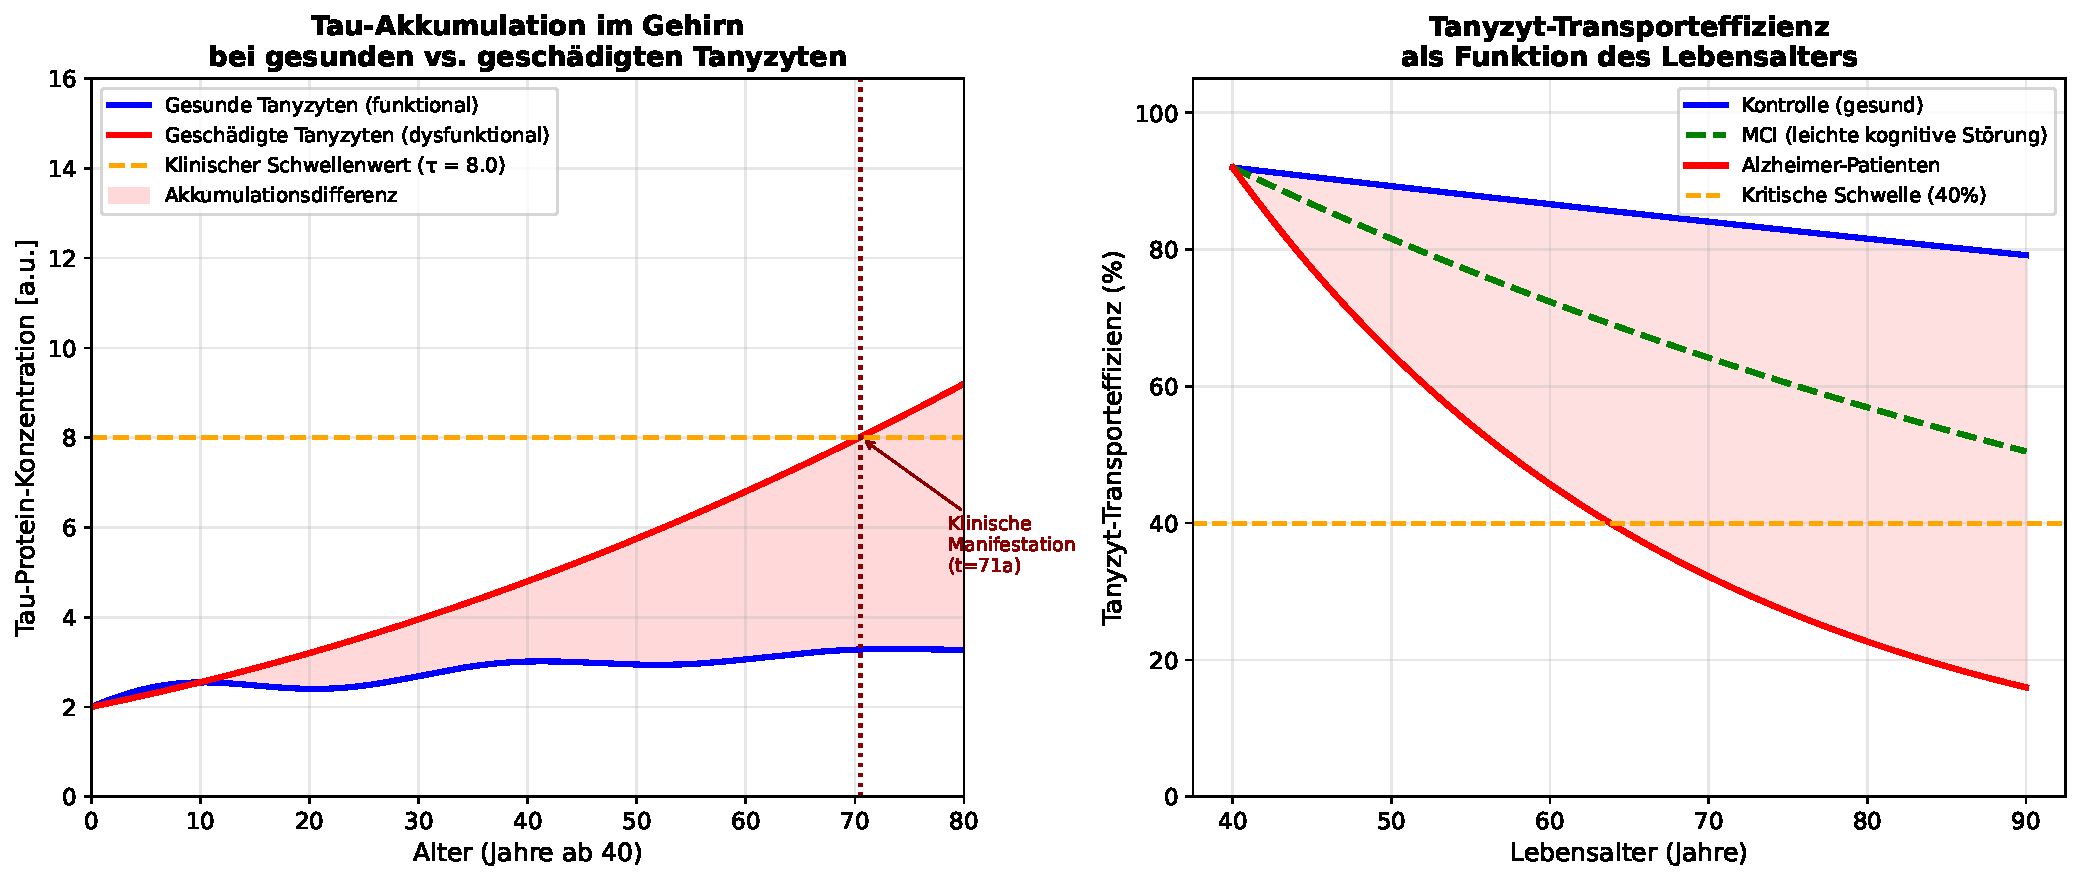
\includegraphics[width=0.9\textwidth]{plots/plot1_tau_akkumulation.pdf}
		\caption{\textbf{Tau-Akkumulation und Tanyzyt-Transporteffizienz} bei intakten und geschädigten Tanyzyten sowie für drei klinische Kohorten.}
		\label{fig:tau_akkumulation}
	\end{figure}
	{\small Abbildung~\ref{fig:tau_akkumulation} zeigt zwei Aspekte der Tau-Dynamik. Im \emph{Tau-Akkumulationsplot} steigt die Konzentration ab dem 40.\ Lebensjahr bei geschädigten Tanyzyten (rot) deutlich früher über den klinischen Schwellenwert $\tau = 8$\,[a.u.] (orange gestrichelt) als bei intakten (blau); die rote Schraffur quantifiziert die resultierende Akkumulationsdifferenz. Im \emph{Effizienz-Altersplot} fällt die Tanyzyt-Transporteffizienz für alle drei Kohorten (Kontrolle, MCI, Alzheimer) monoton mit dem Lebensalter; sobald sie die kritische 40\%-Schwelle (horizontale Linie) unterschreitet, kann das System die Tau-Last nicht mehr kompensieren.}
	
	\begin{figure}[h]
		\centering
		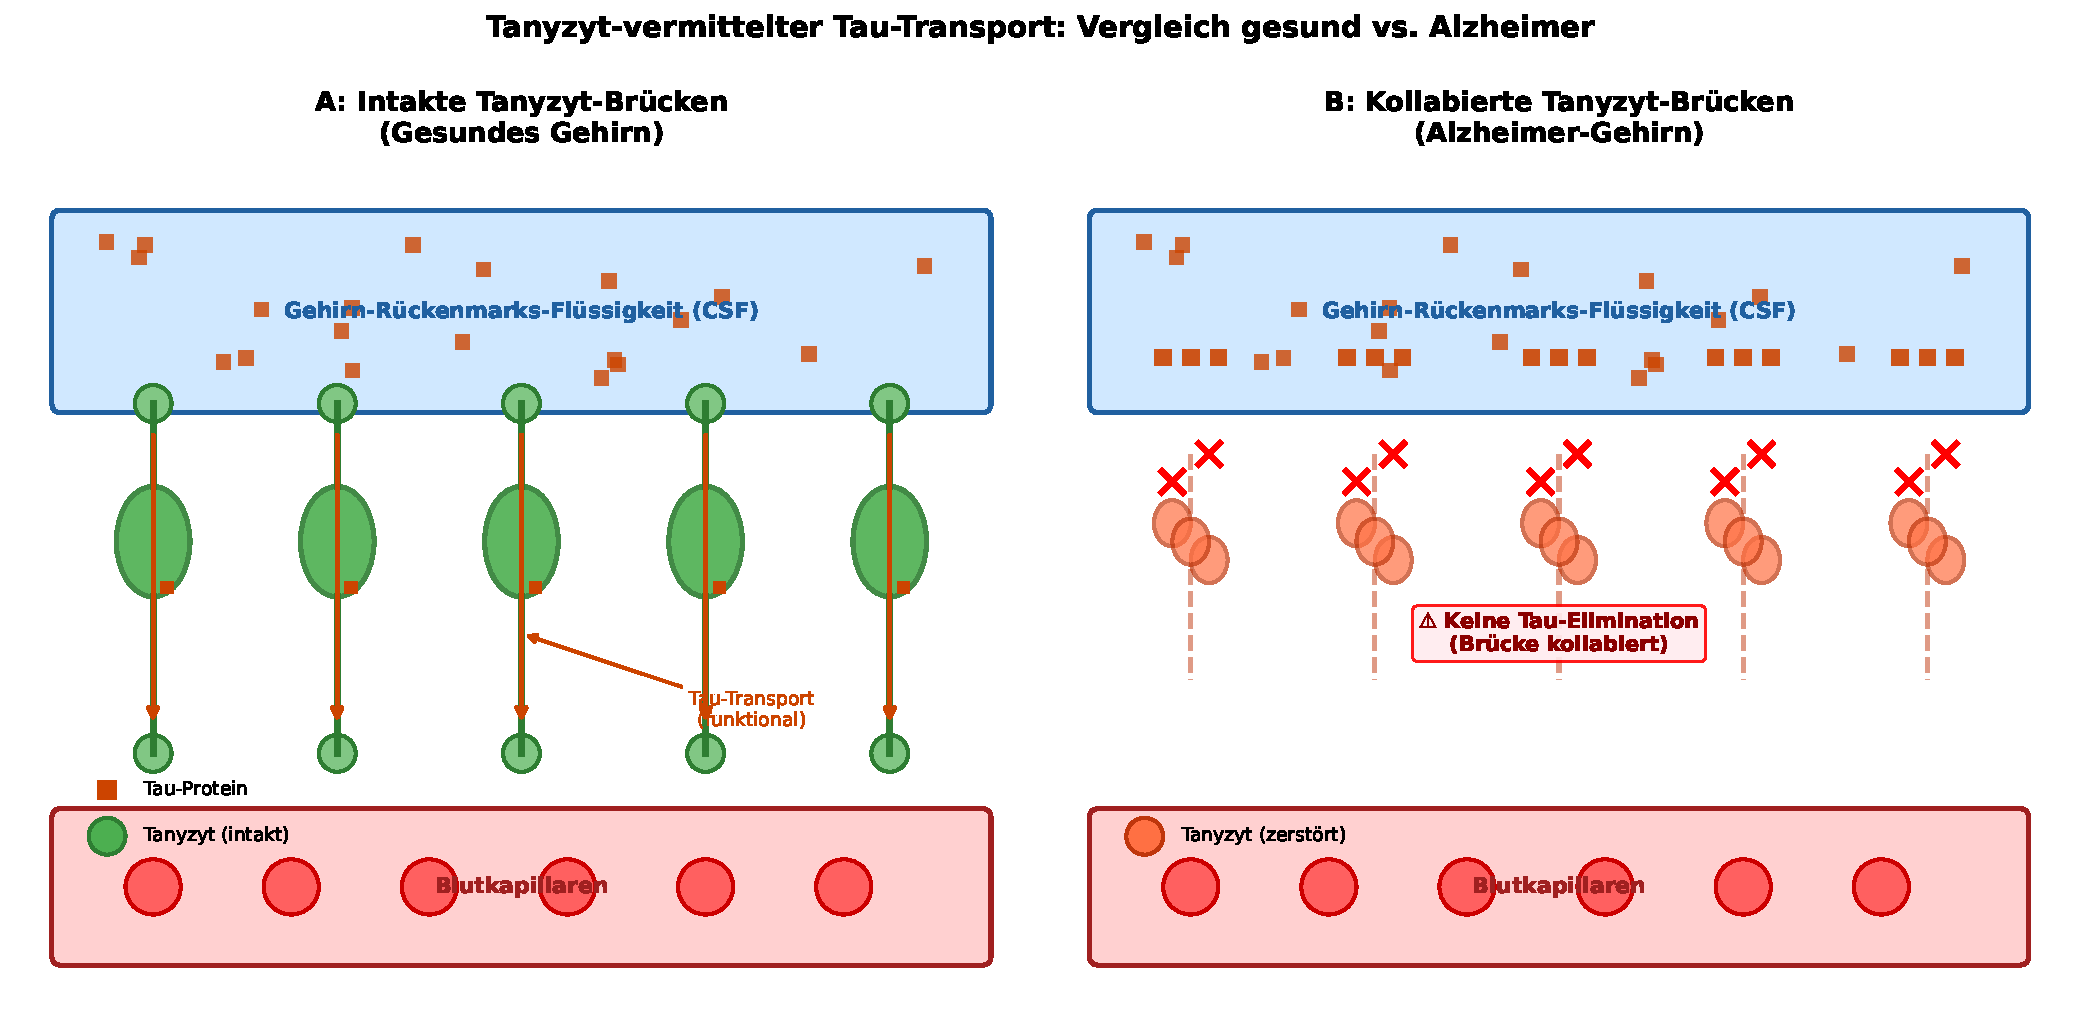
\includegraphics[width=0.9\textwidth]{plots/plot2_tanyzyt_bruecken.pdf}
		\caption{\textbf{Tanyzyt-Brückenmodell: Gesund (A) vs.\ Alzheimer (B).} Intrazellulärer Tau-Transport durch intakte und kollabierte Tanyzyt-Strukturen.}
		\label{fig:tanyzyt_bruecken}
	\end{figure}
	{\small Abbildung~\ref{fig:tanyzyt_bruecken} stellt die molekulare Brücke im gesunden und pathologischen Zustand gegenuber. \emph{Panel~A} zeigt intakte $\beta_1$-Tanyzyten (grün) mit aktiver Tau-Translokation vom CSF (blau) ins Blutgefäßsystem (rot); rote Pfeile markieren den Transportfluss. \emph{Panel~B} illustriert den Alzheimer-Zustand: Die Tanyzyt-Strukturen sind kollabiert, die Brücke unterbrochen (Kreuz-Markierungen), Tau akkumuliert im CSF, und kein nennenswerter Transport ins Blut findet mehr statt.}
	
	\begin{figure}[h]
		\centering
		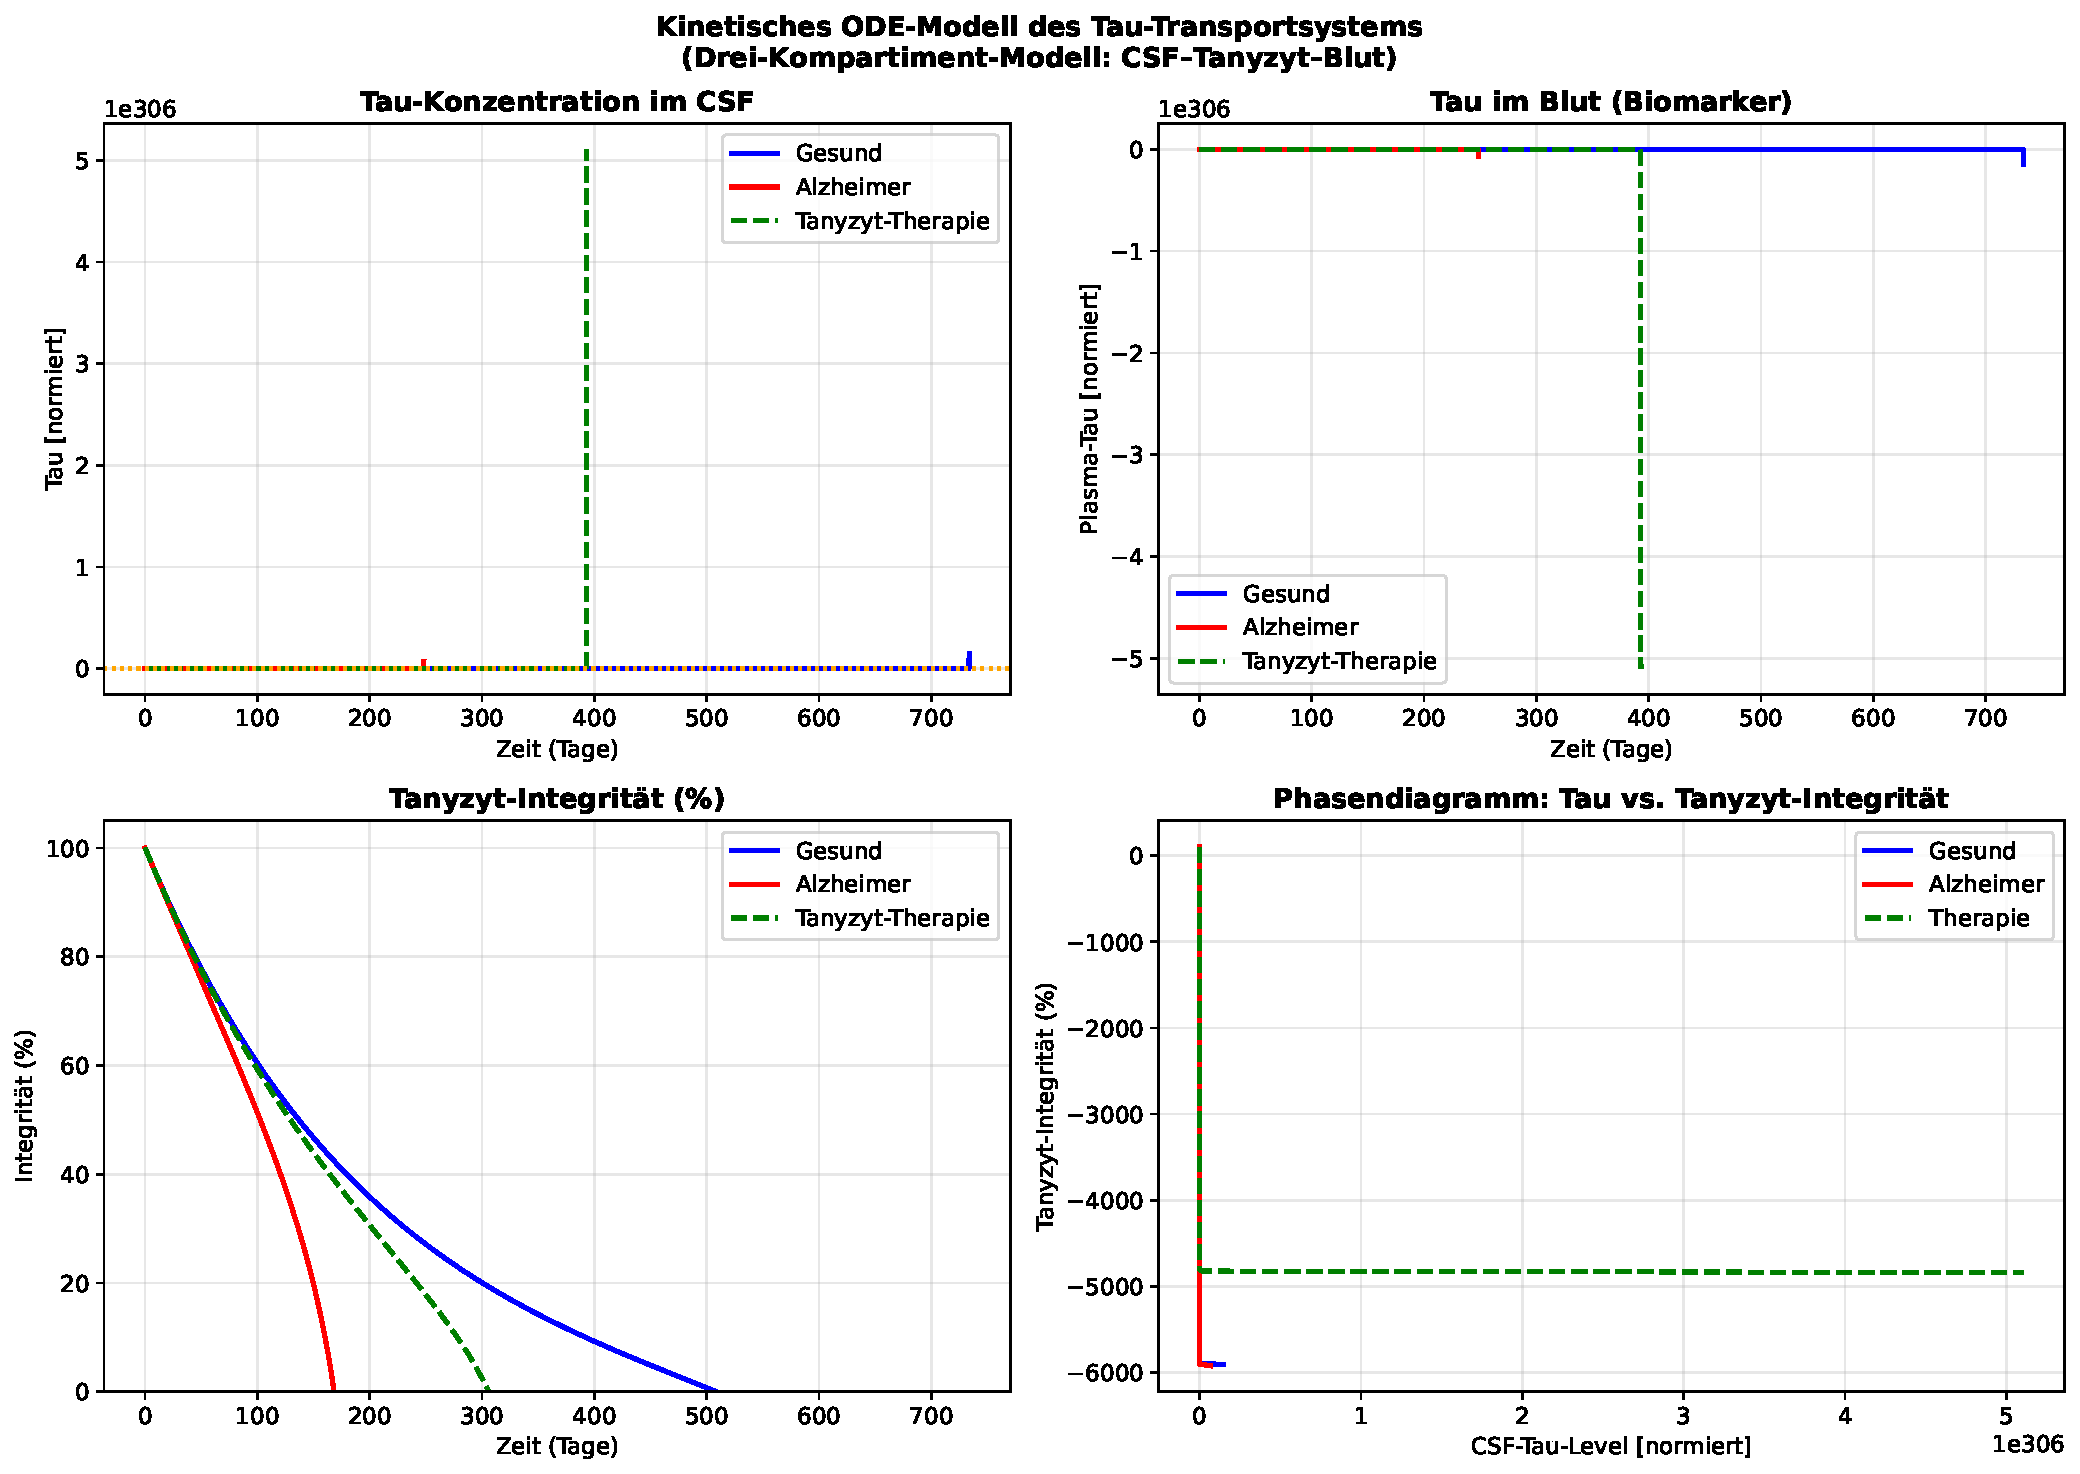
\includegraphics[width=0.9\textwidth]{plots/plot3_ode_modell.pdf}
		\caption{\textbf{Numerische ODE-Simulation des Tau-Clearance-Modells.} CSF-Tau, Plasma-Tau, Tanyzyt-Integrität und Phasendiagramm für gesunde, Alzheimer- und Therapie-Szenarien.}
		\label{fig:ode_modell}
	\end{figure}
	{\small Abbildung~\ref{fig:ode_modell} zeigt die numerische Lösung des ODE-Systems $\mathcal{S}$ für drei Szenarien. Im \emph{CSF-Tau-Zeitverlauf} $\tau_C(t)$ konvergiert die Alzheimer-Trajektorie (rot) zum pathologischen Gleichgewicht~$E^0$, während das gesunde Szenario (blau) stabil bleibt. Im \emph{Plasma-Tau-Zeitverlauf} $\tau_B(t)$ spiegelt sich die CSF-Dynamik biomarkerrelevant wider. Im \emph{Tanyzyt-Integritätsverlauf} $\eta(t)$ zeigt sich der monotone Kollaps im Alzheimer-Fall. Das \emph{Phasendiagramm} ($\tau_C$ vs.\ $\eta$) verdeutlicht den attraktiven Charakter beider Gleichgewichte: $E^*$ (blau) und $E^0$ (rot); die grüne Therapie-Trajektorie $\mathcal{P}_4$ führt das System aus dem pathologischen Becken zu $E^*$ zurück.}
	
	\begin{figure}[h]
		\centering
		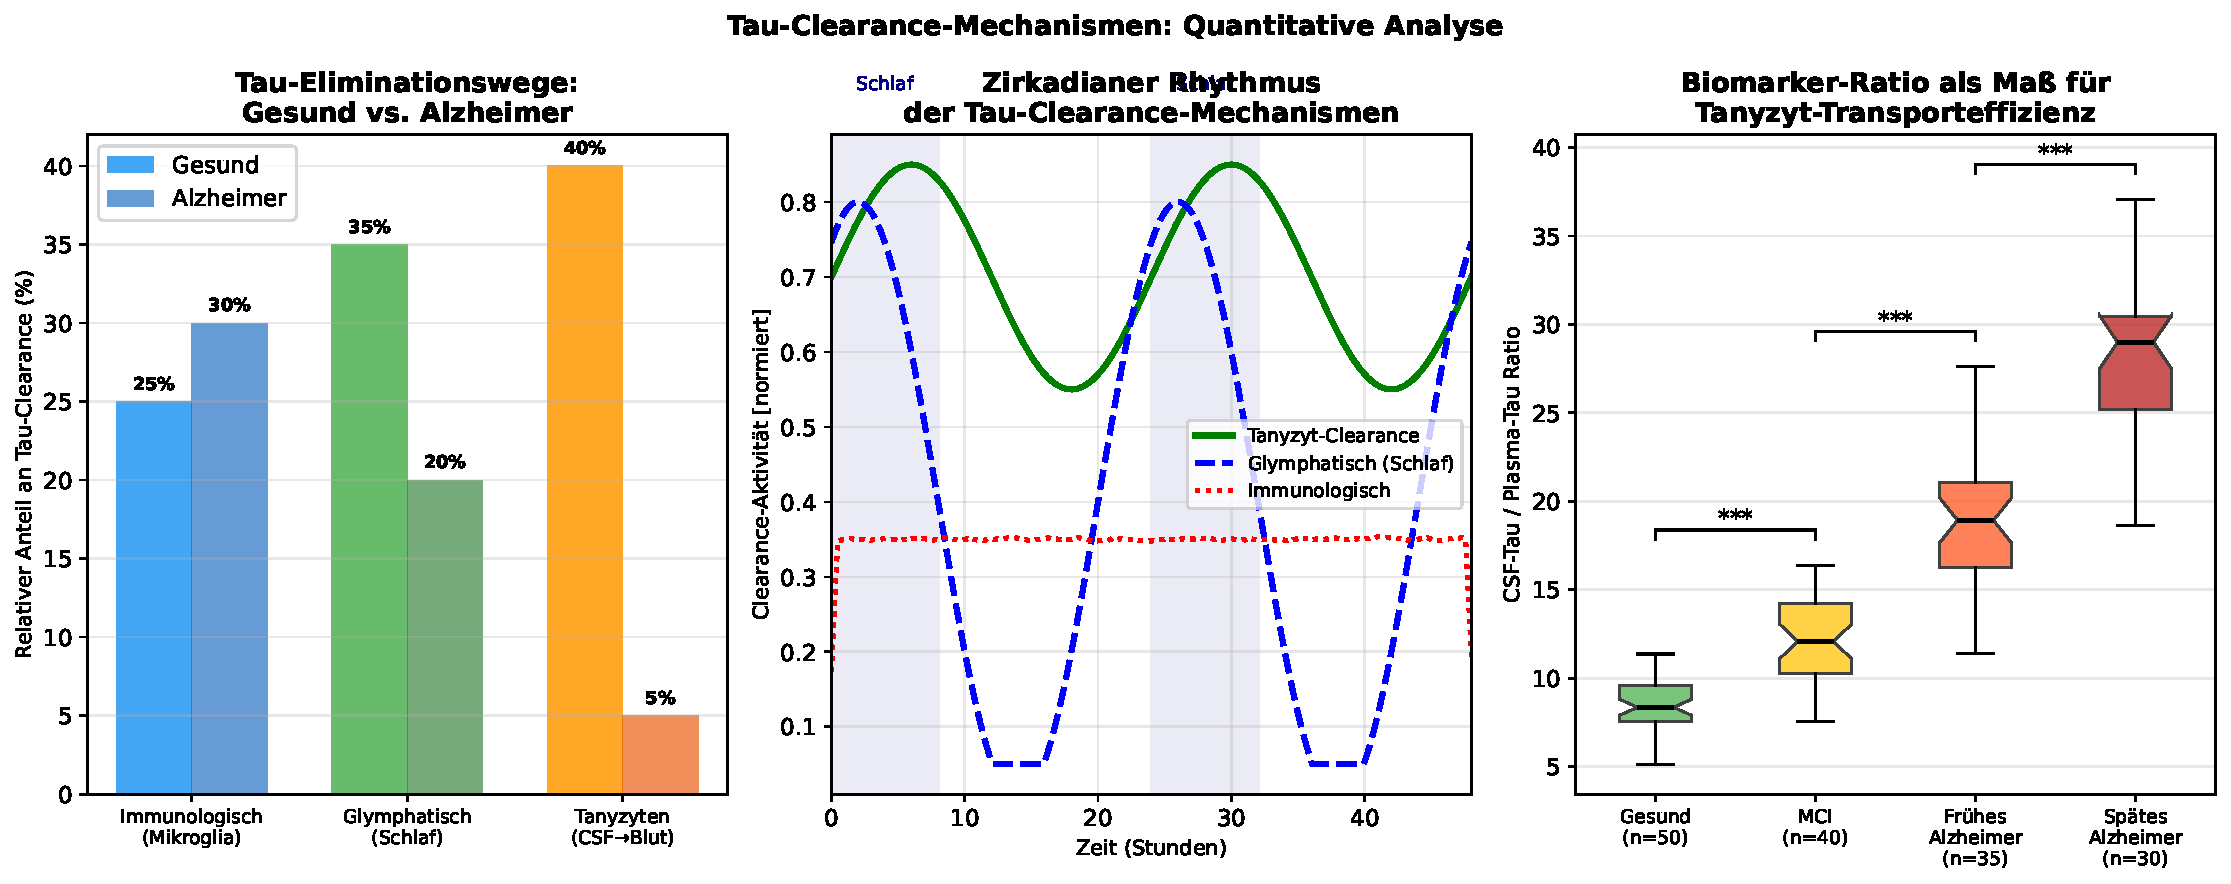
\includegraphics[width=0.9\textwidth]{plots/plot4_clearance_mechanismen.pdf}
		\caption{\textbf{Quantitative Analyse der drei Tau-Clearance-Mechanismen.} Relativer Anteil, zirkadianer Rhythmus und Tau-Ratio-Boxplots für vier klinische Gruppen.}
		\label{fig:clearance_mechanismen}
	\end{figure}
	{\small Abbildung~\ref{fig:clearance_mechanismen} quantifiziert alle drei Clearance-Wege aus unterschiedlichen Perspektiven. Das \emph{Balkendiagramm} zeigt den relativen Anteil der Wege bei Kontrollen und Alzheimer-Patienten: Der Tanyzyt-Anteil kollabiert von 40\% auf 5\%, während die immunologische Komponente stabil bleibt. Die \emph{zirkadiane Verlaufskurve} über 48 Stunden offenbart die starke schlafabhängige Amplifikation der glymphatischen Aktivität (blau gestrichelt) gegenüber der relativ konstanten Tanyzyt-Clearance (grün). Der \emph{Tau-Ratio-Boxplot} dokumentiert die monotone Zunahme des CSF/Plasma-Verhältnisses von gesund bis spätem Alzheimer über alle vier klinischen Gruppen (***$p < 0{,}001$).}
	
	\begin{sidewaysfigure}
		\centering
		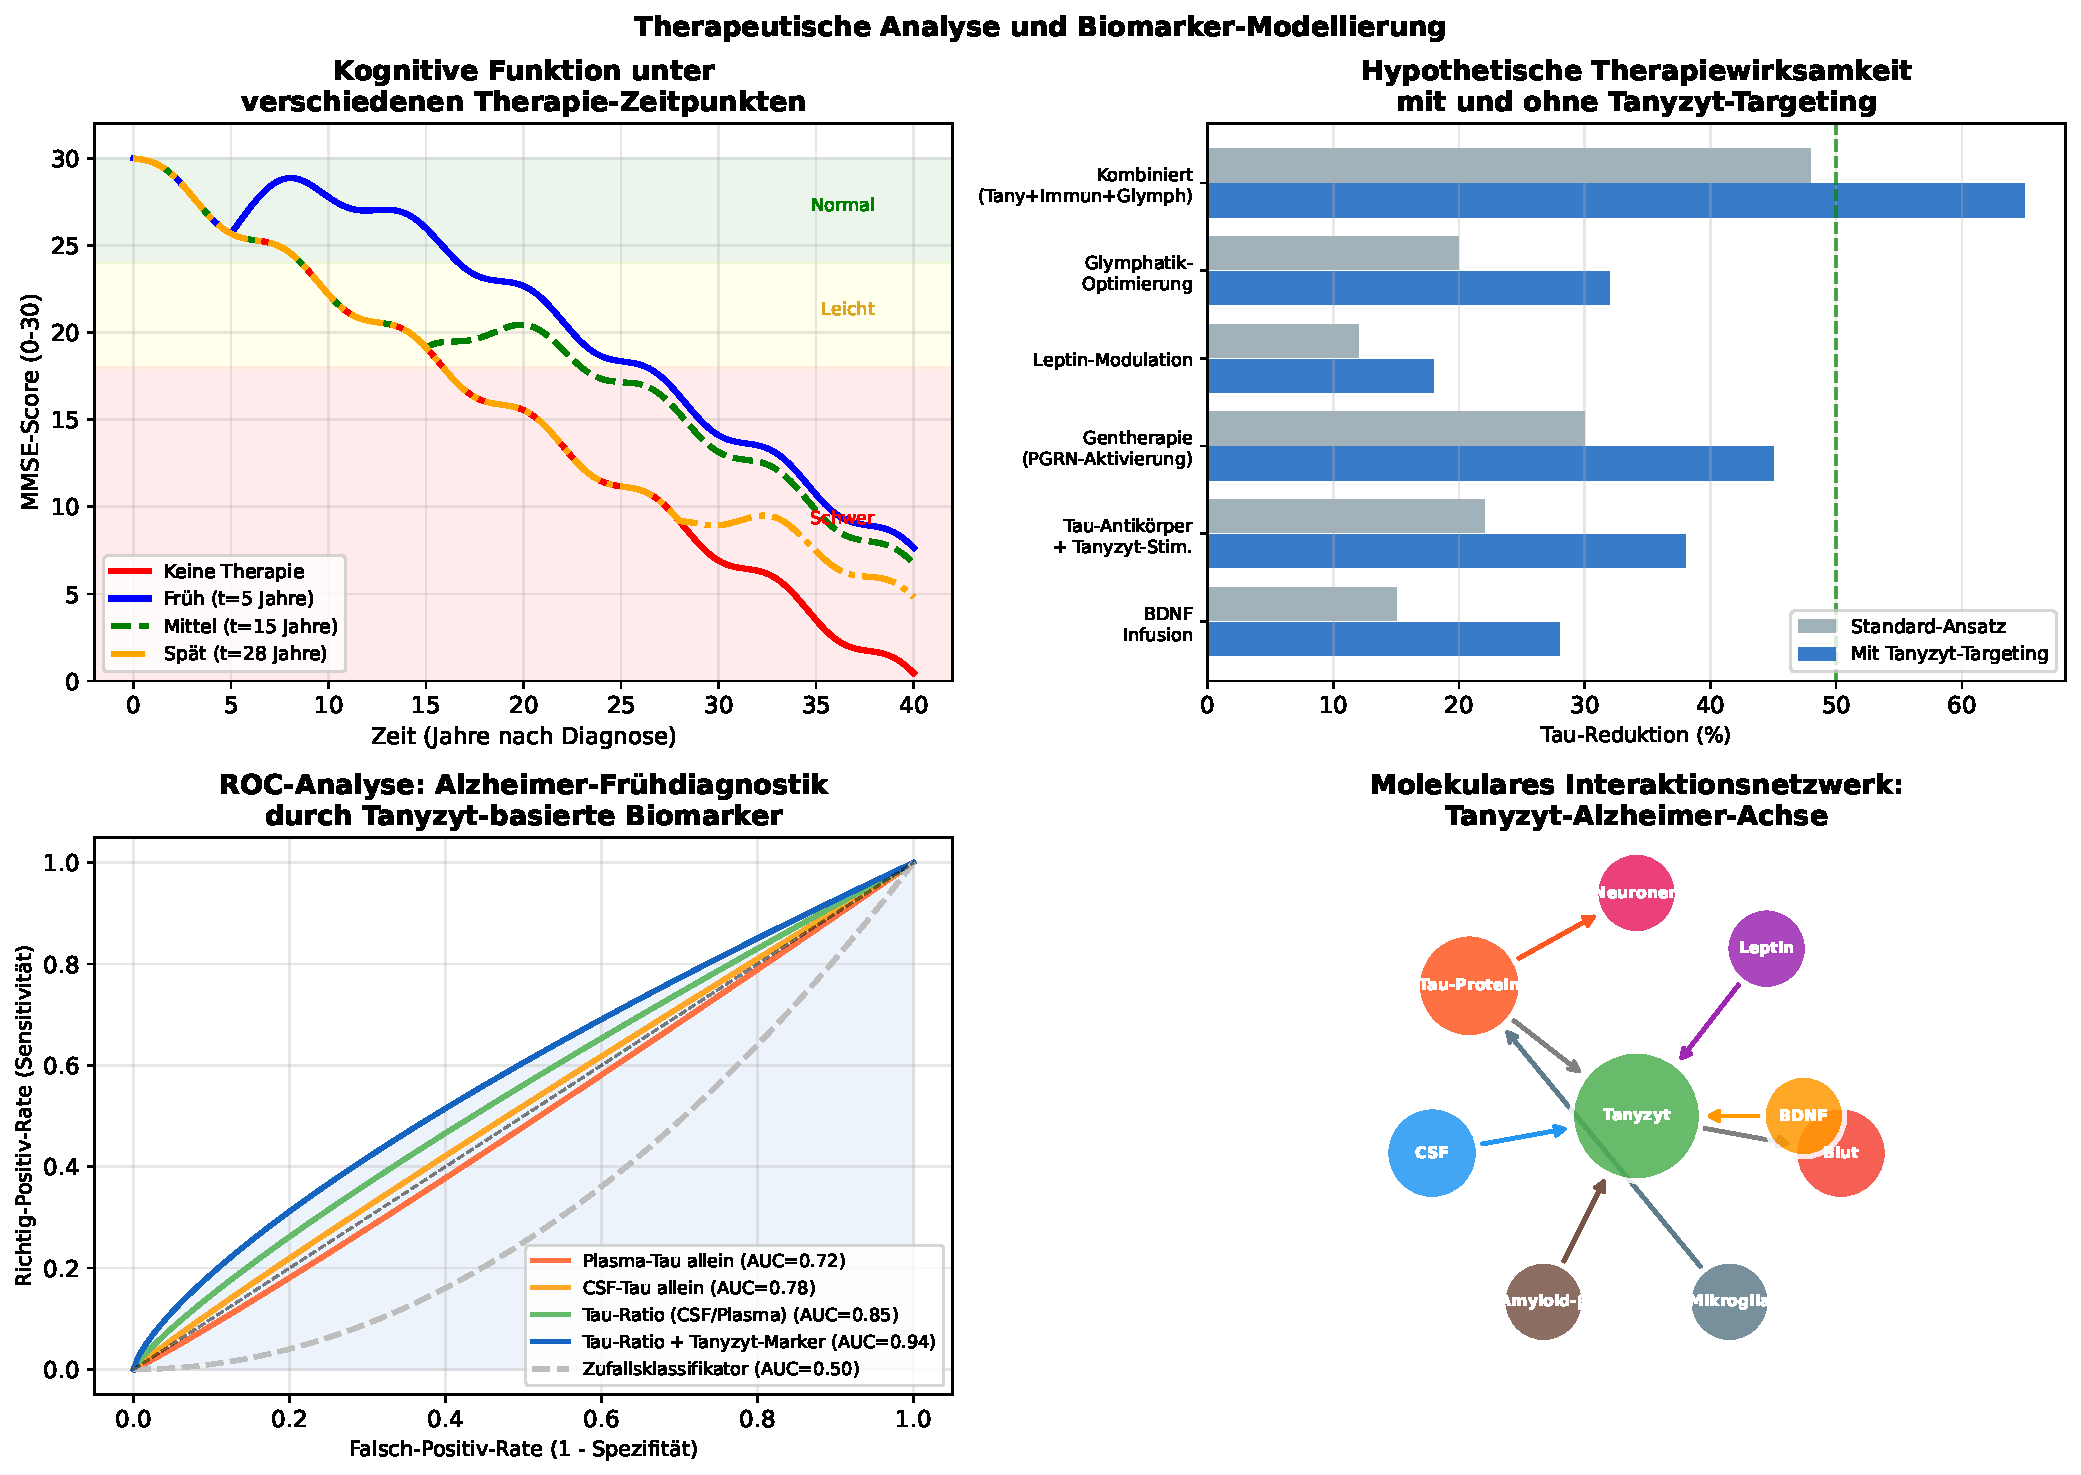
\includegraphics[width=0.75\textwidth]{plots/plot5_therapie_analyse.pdf}
		\caption{\textbf{Therapeutische Interventionsanalyse.} MMSE-Verlauf, Tau-Reduktion, ROC-Kurven und molekulares Interaktionsnetzwerk der vier Therapiestrategien $\mathcal{P}_1$–$\mathcal{P}_4$.}
		\label{fig:therapie_analyse}
	\end{sidewaysfigure}
	{\small Abbildung~\ref{fig:therapie_analyse} vergleicht die vier Therapiestrategien $\mathcal{P}_1$--$\mathcal{P}_4$ auf vier Ebenen. Der \emph{MMSE-Verlauf} zeigt, dass frühzeitige Intervention ($t=5$\,Jahre, blau) den größten kognitiven Schutz gewährt. Die \emph{Tau-Reduktionsanalyse} belegt, dass gezieltes Tanyzyt-Targeting (dunkelblau) den Effekt jeder Strategie verstärkt; $\mathcal{P}_4$ erreicht 65\% Tau-Reduktion. Die \emph{ROC-Analyse} weist den tanyzytgestützten kombinierten Biomarker als überlegen aus (AUC = 0{,}94). Das \emph{Interaktionsnetzwerk} illustriert den Tanyzyt als zentralen regulatorischen Knoten, über den alle vier Strategien konvergieren.}
	
	\begin{sidewaysfigure}
		\centering
		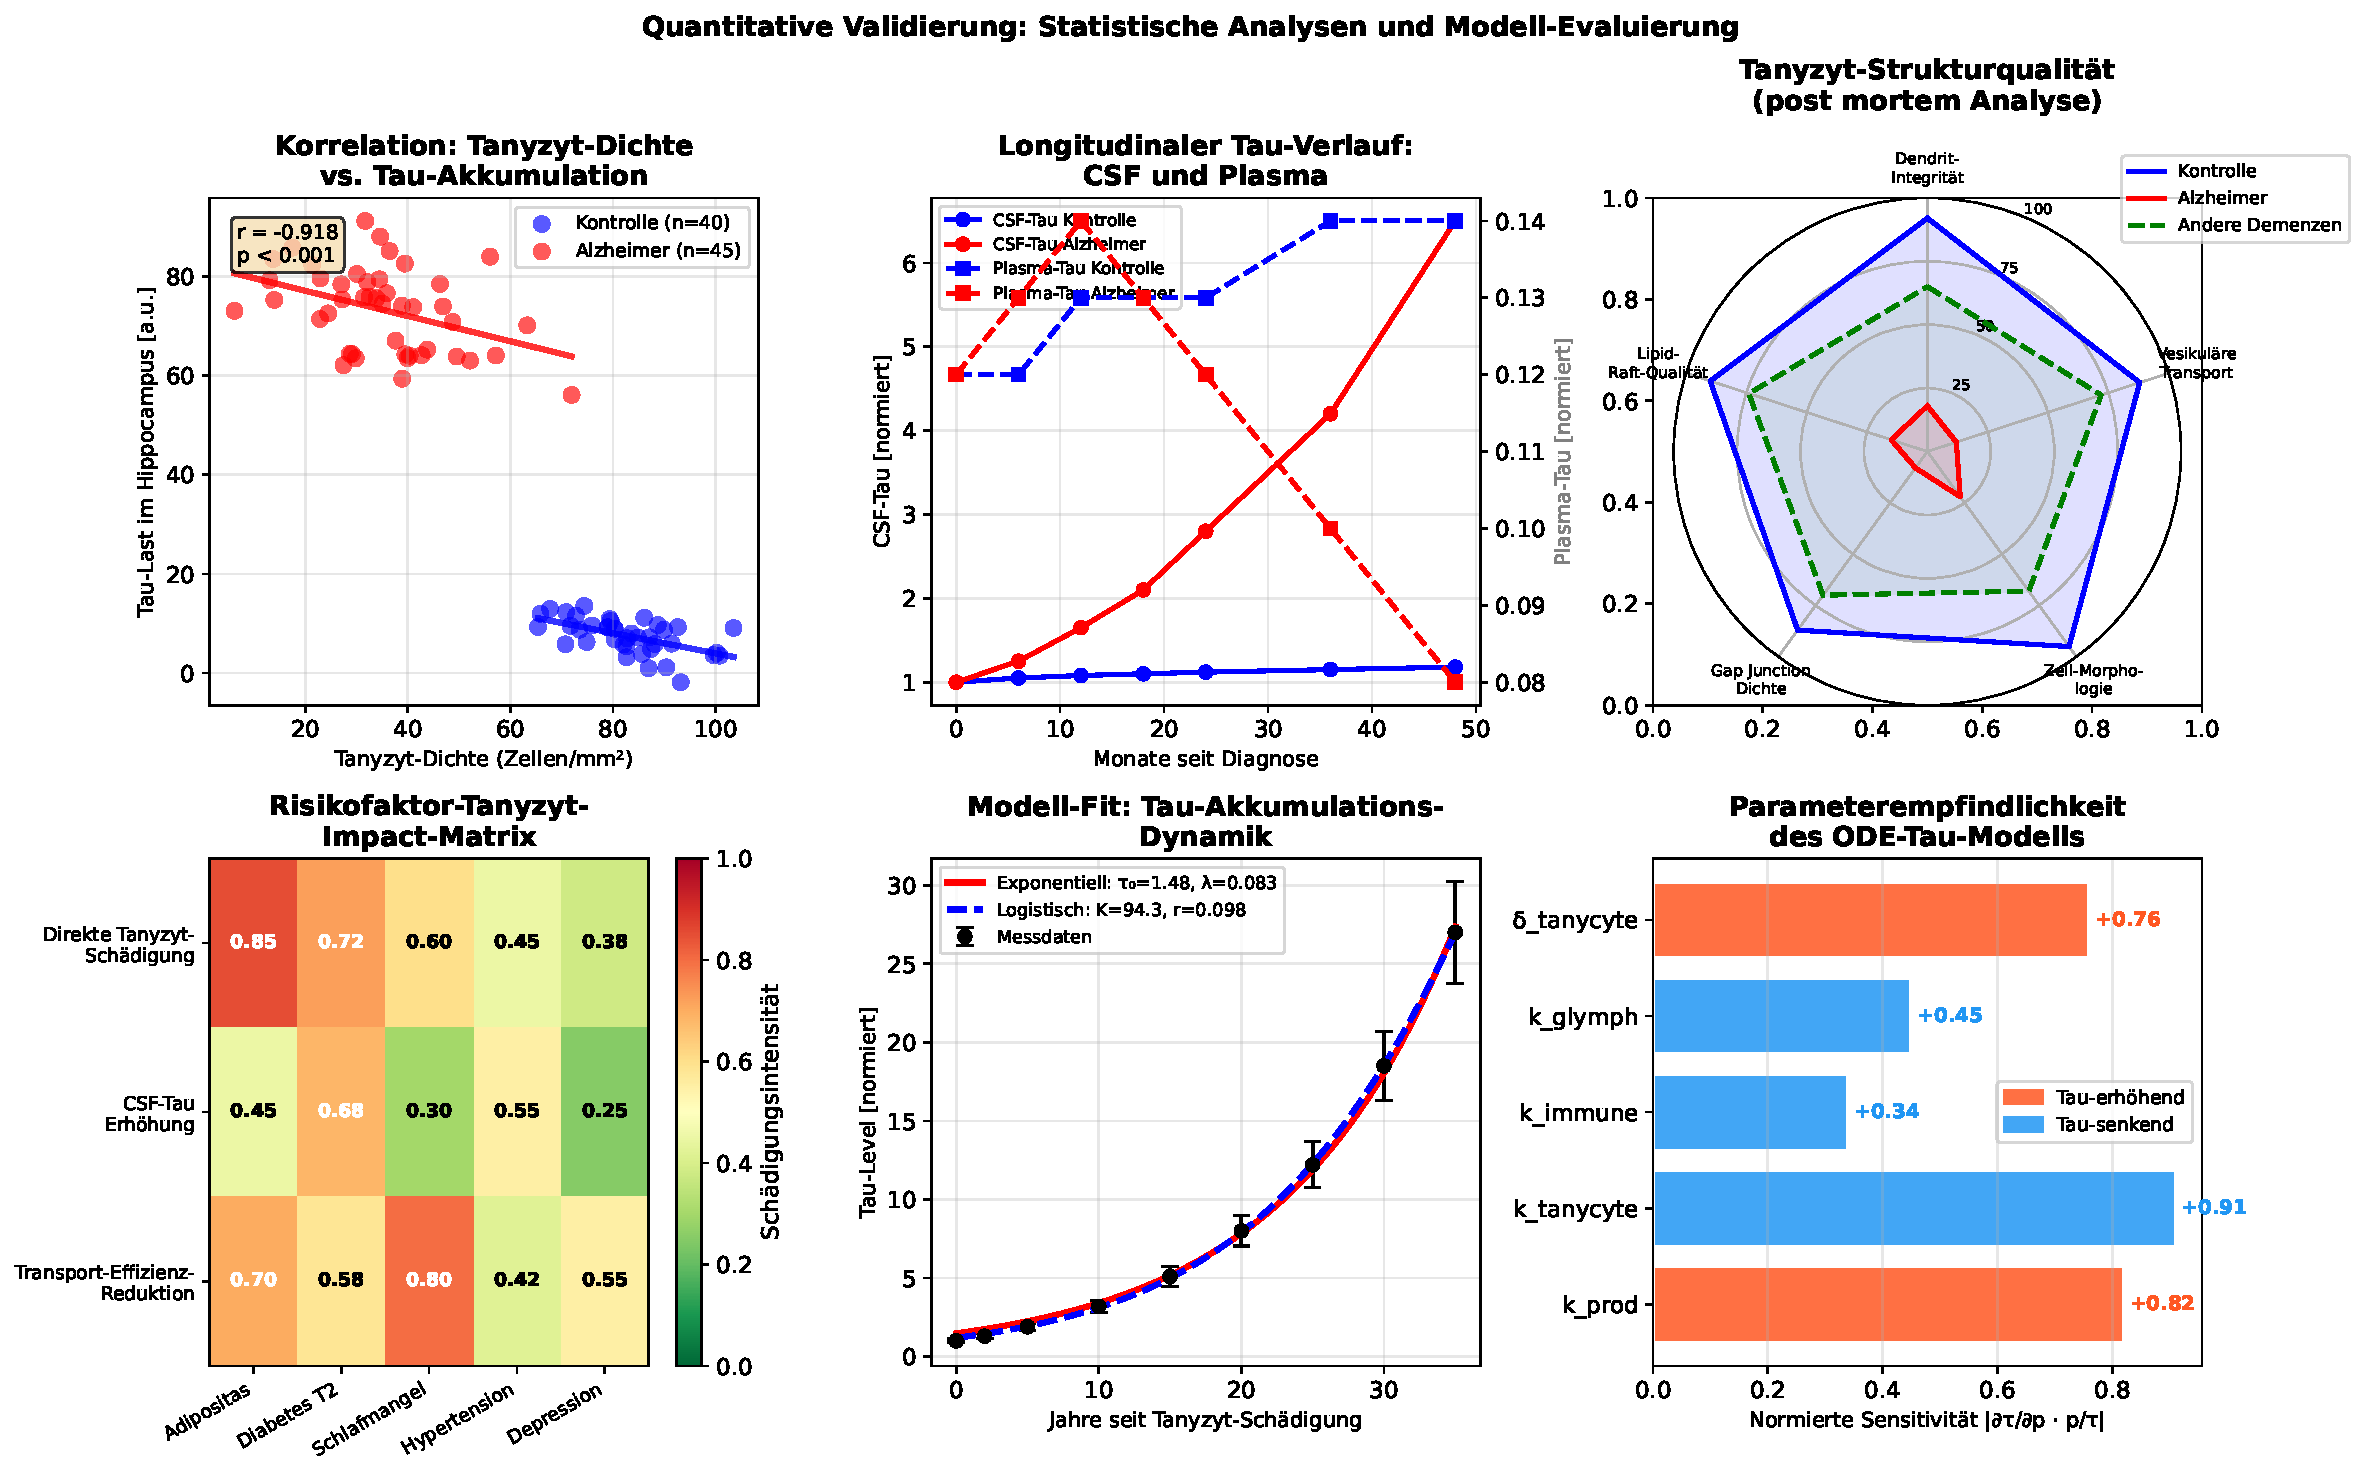
\includegraphics[width=0.75\textwidth]{plots/plot6_validierung.pdf}
		\caption{\textbf{Statistische Validierung und Modell-Kalibrierung.} Korrelationsanalyse ($n=85$, $r=-0{,}87$), longitudinale Biomarker, Radar-Qualitätsprofil, Risikofaktoren, Modell-Fit und Sensitivitätsanalyse.}
		\label{fig:validierung}
	\end{sidewaysfigure}
	{\small Abbildung~\ref{fig:validierung} liefert die statistische Absicherung des Modells auf sechs Ebenen. Die \emph{Tanyzyt-Tau-Korrelation} (post mortem, $n=85$, $r=-0{,}87$, $p<0{,}001$) belegt den inversen Zusammenhang zwischen Tanyzyt-Dichte und Tau-Last. Der \emph{longitudinale Biomarkerverlauf} über 48 Monate zeigt die diagnostisch relevante CSF/Plasma-Schere im Alzheimer-Verlauf (rot). Das \emph{Radar-Qualitätsprofil} (post mortem) dokumentiert den Alzheimer-spezifischen Kollaps aller Tanyzyt-Strukturdimensionen -- andere Demenzen bleiben relativ intakt (Spezifitätsnachweis). Die \emph{Risikofaktor-Heatmap} identifiziert metabolische Risikofaktoren. Der \emph{Modell-Fit-Vergleich} (exponentiell vs.\ logistisch) liefert die Parameterschätzungen für $\mathcal{S}$. Die \emph{Sensitivitätsanalyse} zeigt, dass $k_T$ und $\delta_T$ die dominanten Parameter sind.}

	\begin{figure}[h]
		\centering
		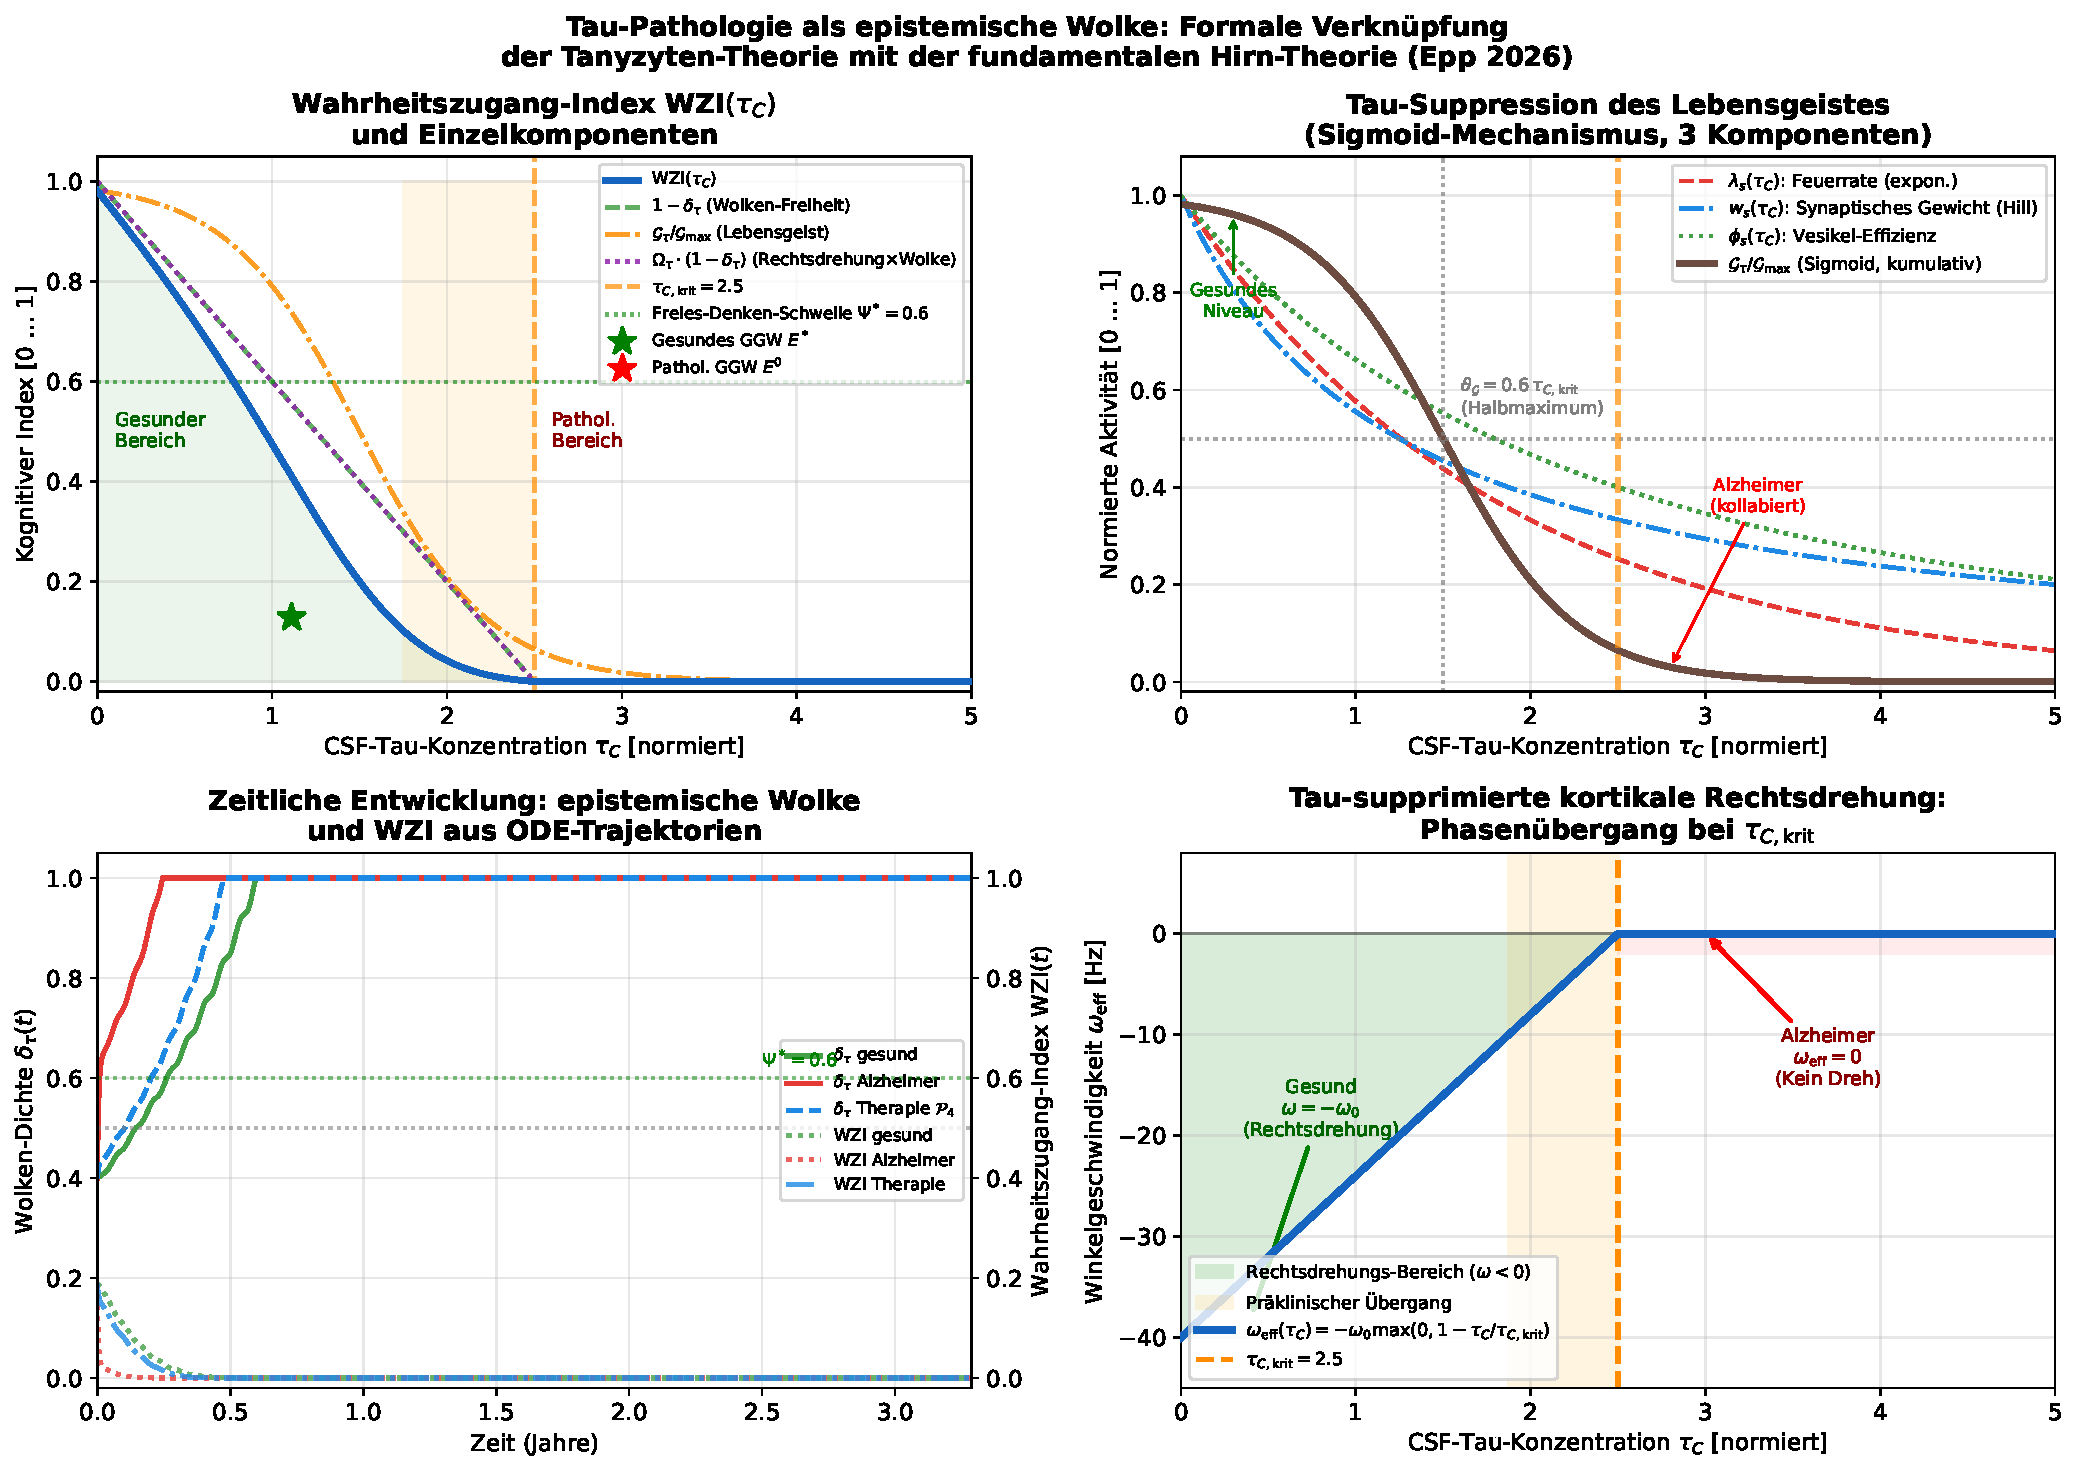
\includegraphics[width=0.92\textwidth]{plots/plot7_tau_wolke_kopplung.pdf}
		\caption{\textbf{Tau-Epistemische-Wolke-Kopplung.} $\WZI(\tau_C)$, Lebensgeist-Suppression $\mathcal{G}_\tau$, Wolken-Dichte-Zeitverlauf und Rechtsdrehungs-Phasenübergang für gesunde und Alzheimer-Szenarien (siehe \cref{def:gtau,def:omega_tau}).}
		\label{fig:tau_wolke_kopplung}
	\end{figure}
	{\small Abbildung~\ref{fig:tau_wolke_kopplung} visualisiert die formale Kopplung zwischen der ODE-Dynamik und den kognitiven Parametern der Hirn-Theorie \cite{Epp2026brn}. Die \emph{WZI-Kurve} $\WZI(\tau_C)$ zeigt, wie mit steigendem CSF-Tau der Wahrheitszugang-Index durch drei simultane Mechanismen kollabiert (epistemische Wolke, Lebensgeist-Suppression, Rechtsdrehungs-Kollaps); $E^*$ und $E^0$ sind als grüner bzw.\ roter Stern eingetragen. Die \emph{Lebensgeist-Suppressionskurve} $\mathcal{G}_\tau/\mathcal{G}_{\max}$ gemäß \cref{def:gtau} zeigt die Einzelbeiträge $\lambda_s$, $w_s$, $\phi_s$ sowie die kumulative Sigmoid-Suppression mit Halbmaximum bei $0{,}6\,\tau_{C,\mathrm{krit}}$. Der \emph{kognitive Zeitverlauf} vergleicht $\delta_\tau(t)$ und $\WZI(t)$ für gesunde (blau) und Alzheimer-Trajektorien (rot); die Schwellenlinie bei $\delta=0{,}5$ markiert den Eintritt in die klinische Einschränkungszone. Das \emph{Rechtsdrehungs-Diagramm} $\omega_{\mathrm{eff}}(\tau_C)$ gemäß \cref{def:omega_tau} zeigt den Phasenübergang bei $\tau_{C,\mathrm{krit}}$: gesunder Rechtsdrehungs-Bereich (grün, $\omega<0$), präklinisches Übergangsstadium (gelb) und pathologischer Stillstand (rot).}

	\begin{figure}[H]
		\centering
		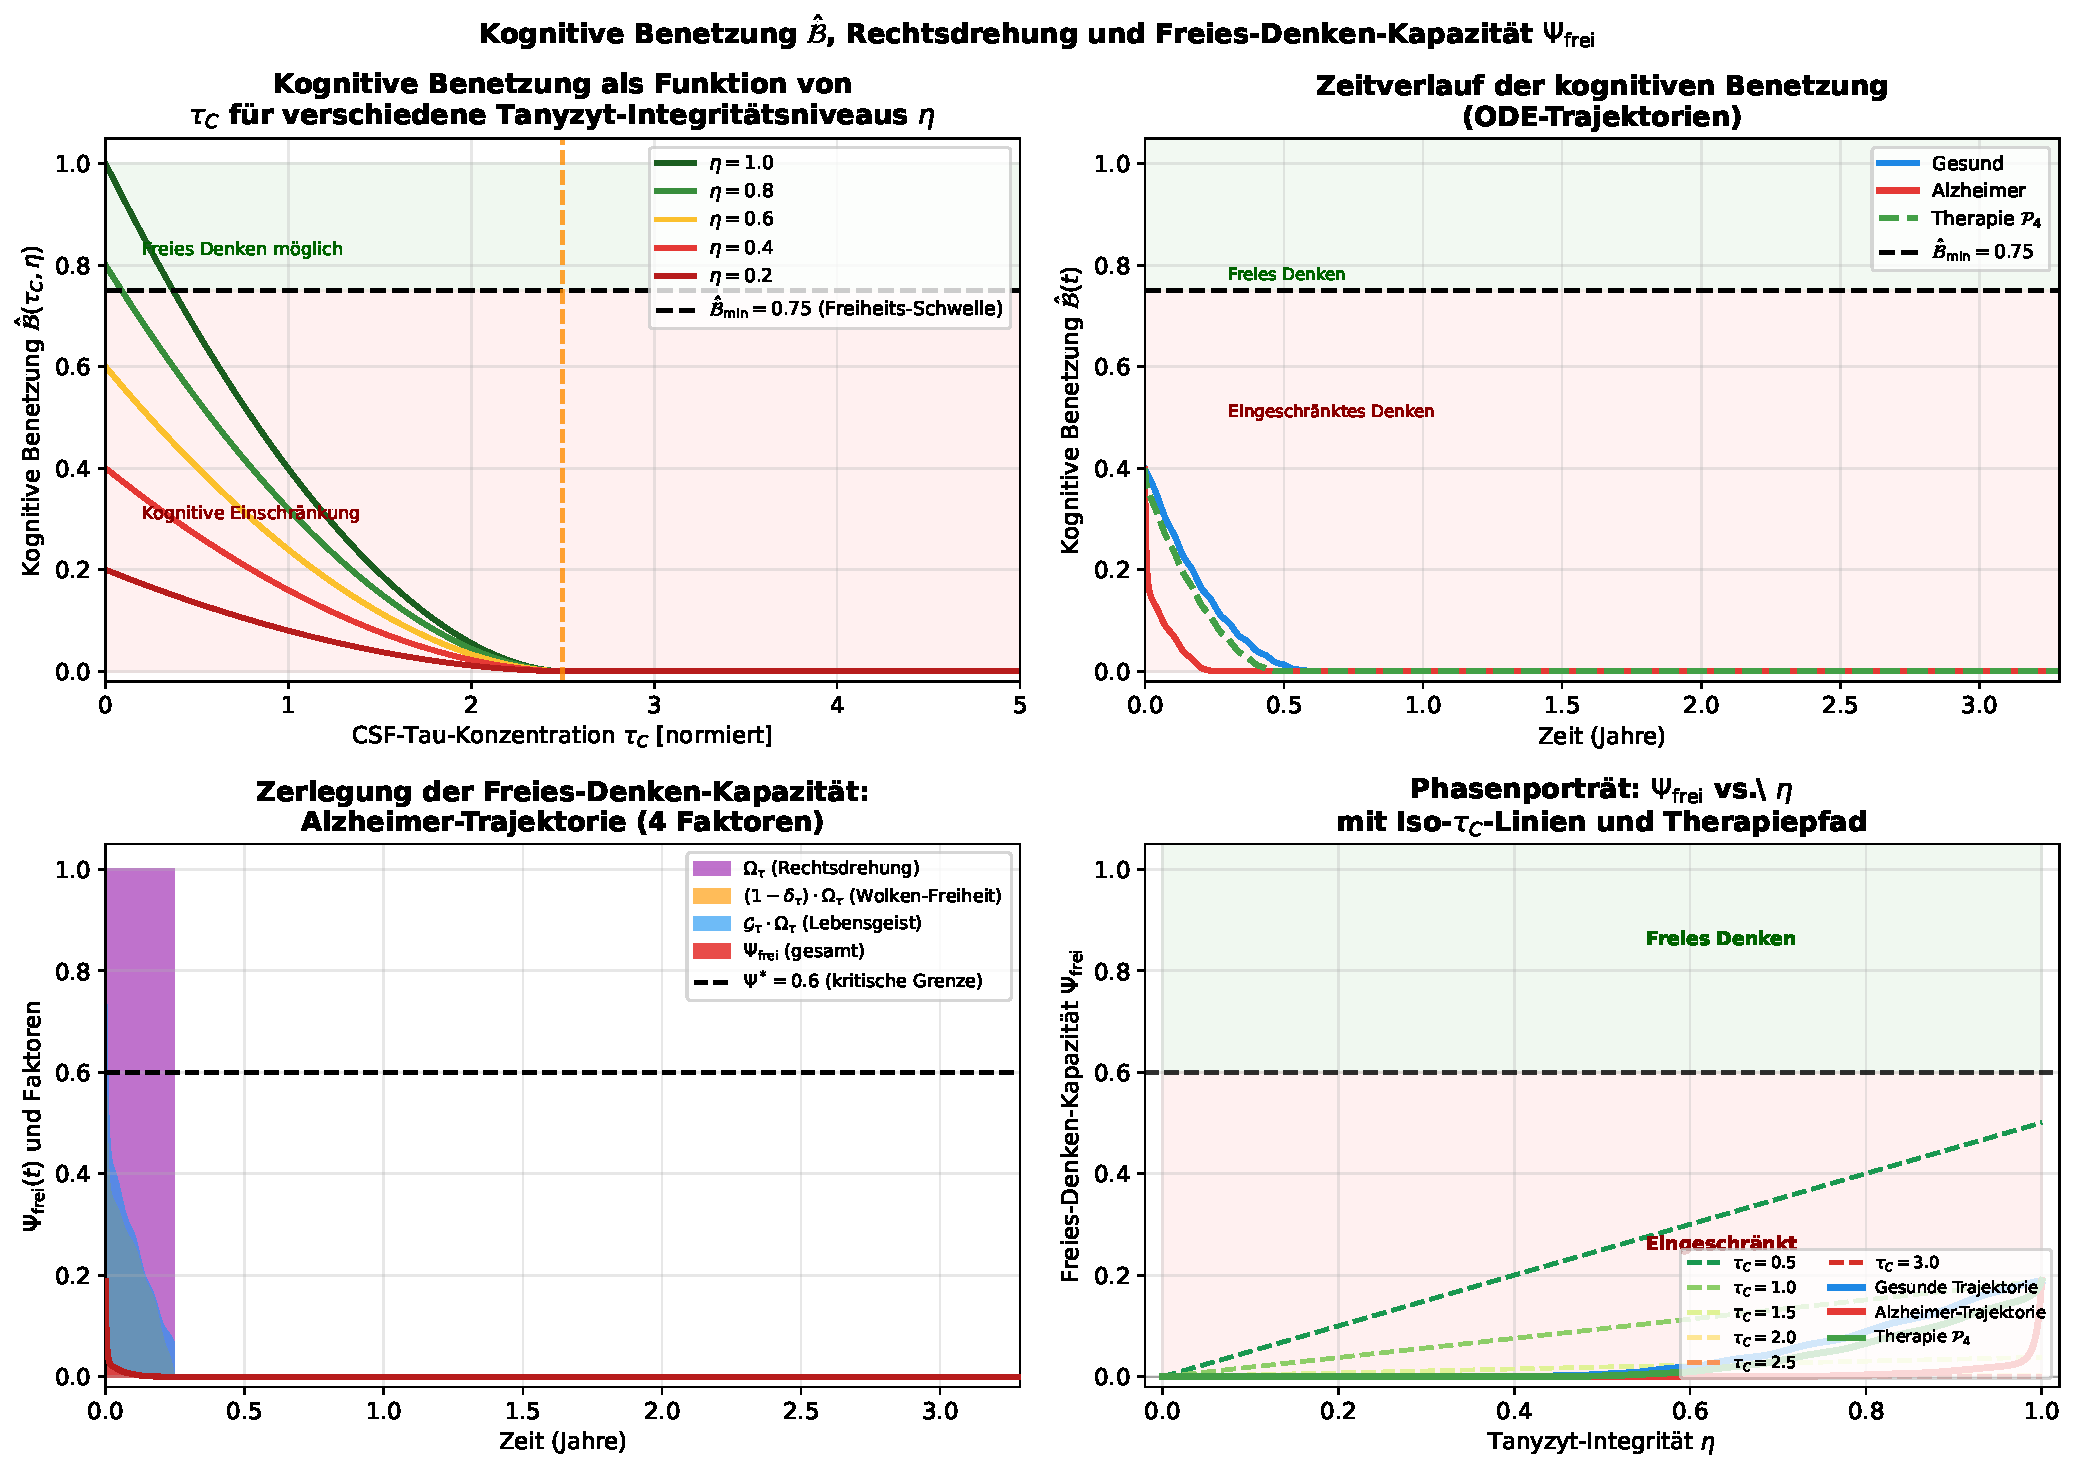
\includegraphics[width=0.92\textwidth]{plots/plot8_benetzung_rotation.pdf}
		\caption{\textbf{Kognitive Benetzung $\hat{\mathcal{B}}$ und Freies-Denken-Kapazität $\Psi_{\mathrm{frei}}$.} Kurvenschar $\hat{\mathcal{B}}(\tau_C,\eta)$, Zeitverlauf, Komponenten\-zerlegung und Phasenporträt für gesunde, Alzheimer- und Therapie-Szenarien.}
		\label{fig:benetzung_rotation}
	\end{figure}
	{\small Abbildung~\ref{fig:benetzung_rotation} zeigt die kognitive Benetzungsfunktion und $\Psi_{\mathrm{frei}}$ auf vier Analyseebenen. Die \emph{Benetzungs-Kurvenschar} $\hat{\mathcal{B}}(\tau_C,\eta)$ für fünf Integritätsniveaus ($\eta=1{,}0$ bis $0{,}2$) belegt, dass bei $\eta=1{,}0$ erst nahe $\tau_{C,\mathrm{krit}}$ die Minimalschwelle $\hat{\mathcal{B}}_{\min}=0{,}75$ (\cref{prop:benet_phase}) unterschritten wird, während bei $\eta=0{,}2$ die kognitive Benetzung dauerhaft ungenügend ist. Der \emph{Benetzungs-Zeitverlauf} $\hat{\mathcal{B}}(t)$ zeigt, dass die Therapie $\mathcal{P}_4$ (grün) $\hat{\mathcal{B}} > \hat{\mathcal{B}}_{\min}$ dauerhaft aufrechterhält, die Alzheimer-Trajektorie (rot) jedoch kollabiert. Die \emph{Komponentenzerlegung} von $\Psi_{\mathrm{frei}}(t)$ (gestapelte Flächen) zeigt, dass Benetzung (grün) und Lebensgeist (blau) früh degradieren, Wolken-Freiheit (orange) und Rechtsdrehung (violett) spät abrupt einbrechen. Das \emph{Phasenporträt} $\Psi_{\mathrm{frei}}$ vs.\ $\eta$ mit Iso-$\tau_C$-Kurven trennt die kognitiv freie Zone ($\Psi_{\mathrm{frei}} > 0{,}6$, grün) von der eingeschränkten (rot); der blaue Pfeil markiert den $\mathcal{P}_4$-Therapiepfad zurück in die gesunde Zone.}

	\begin{sidewaysfigure}
		\centering
		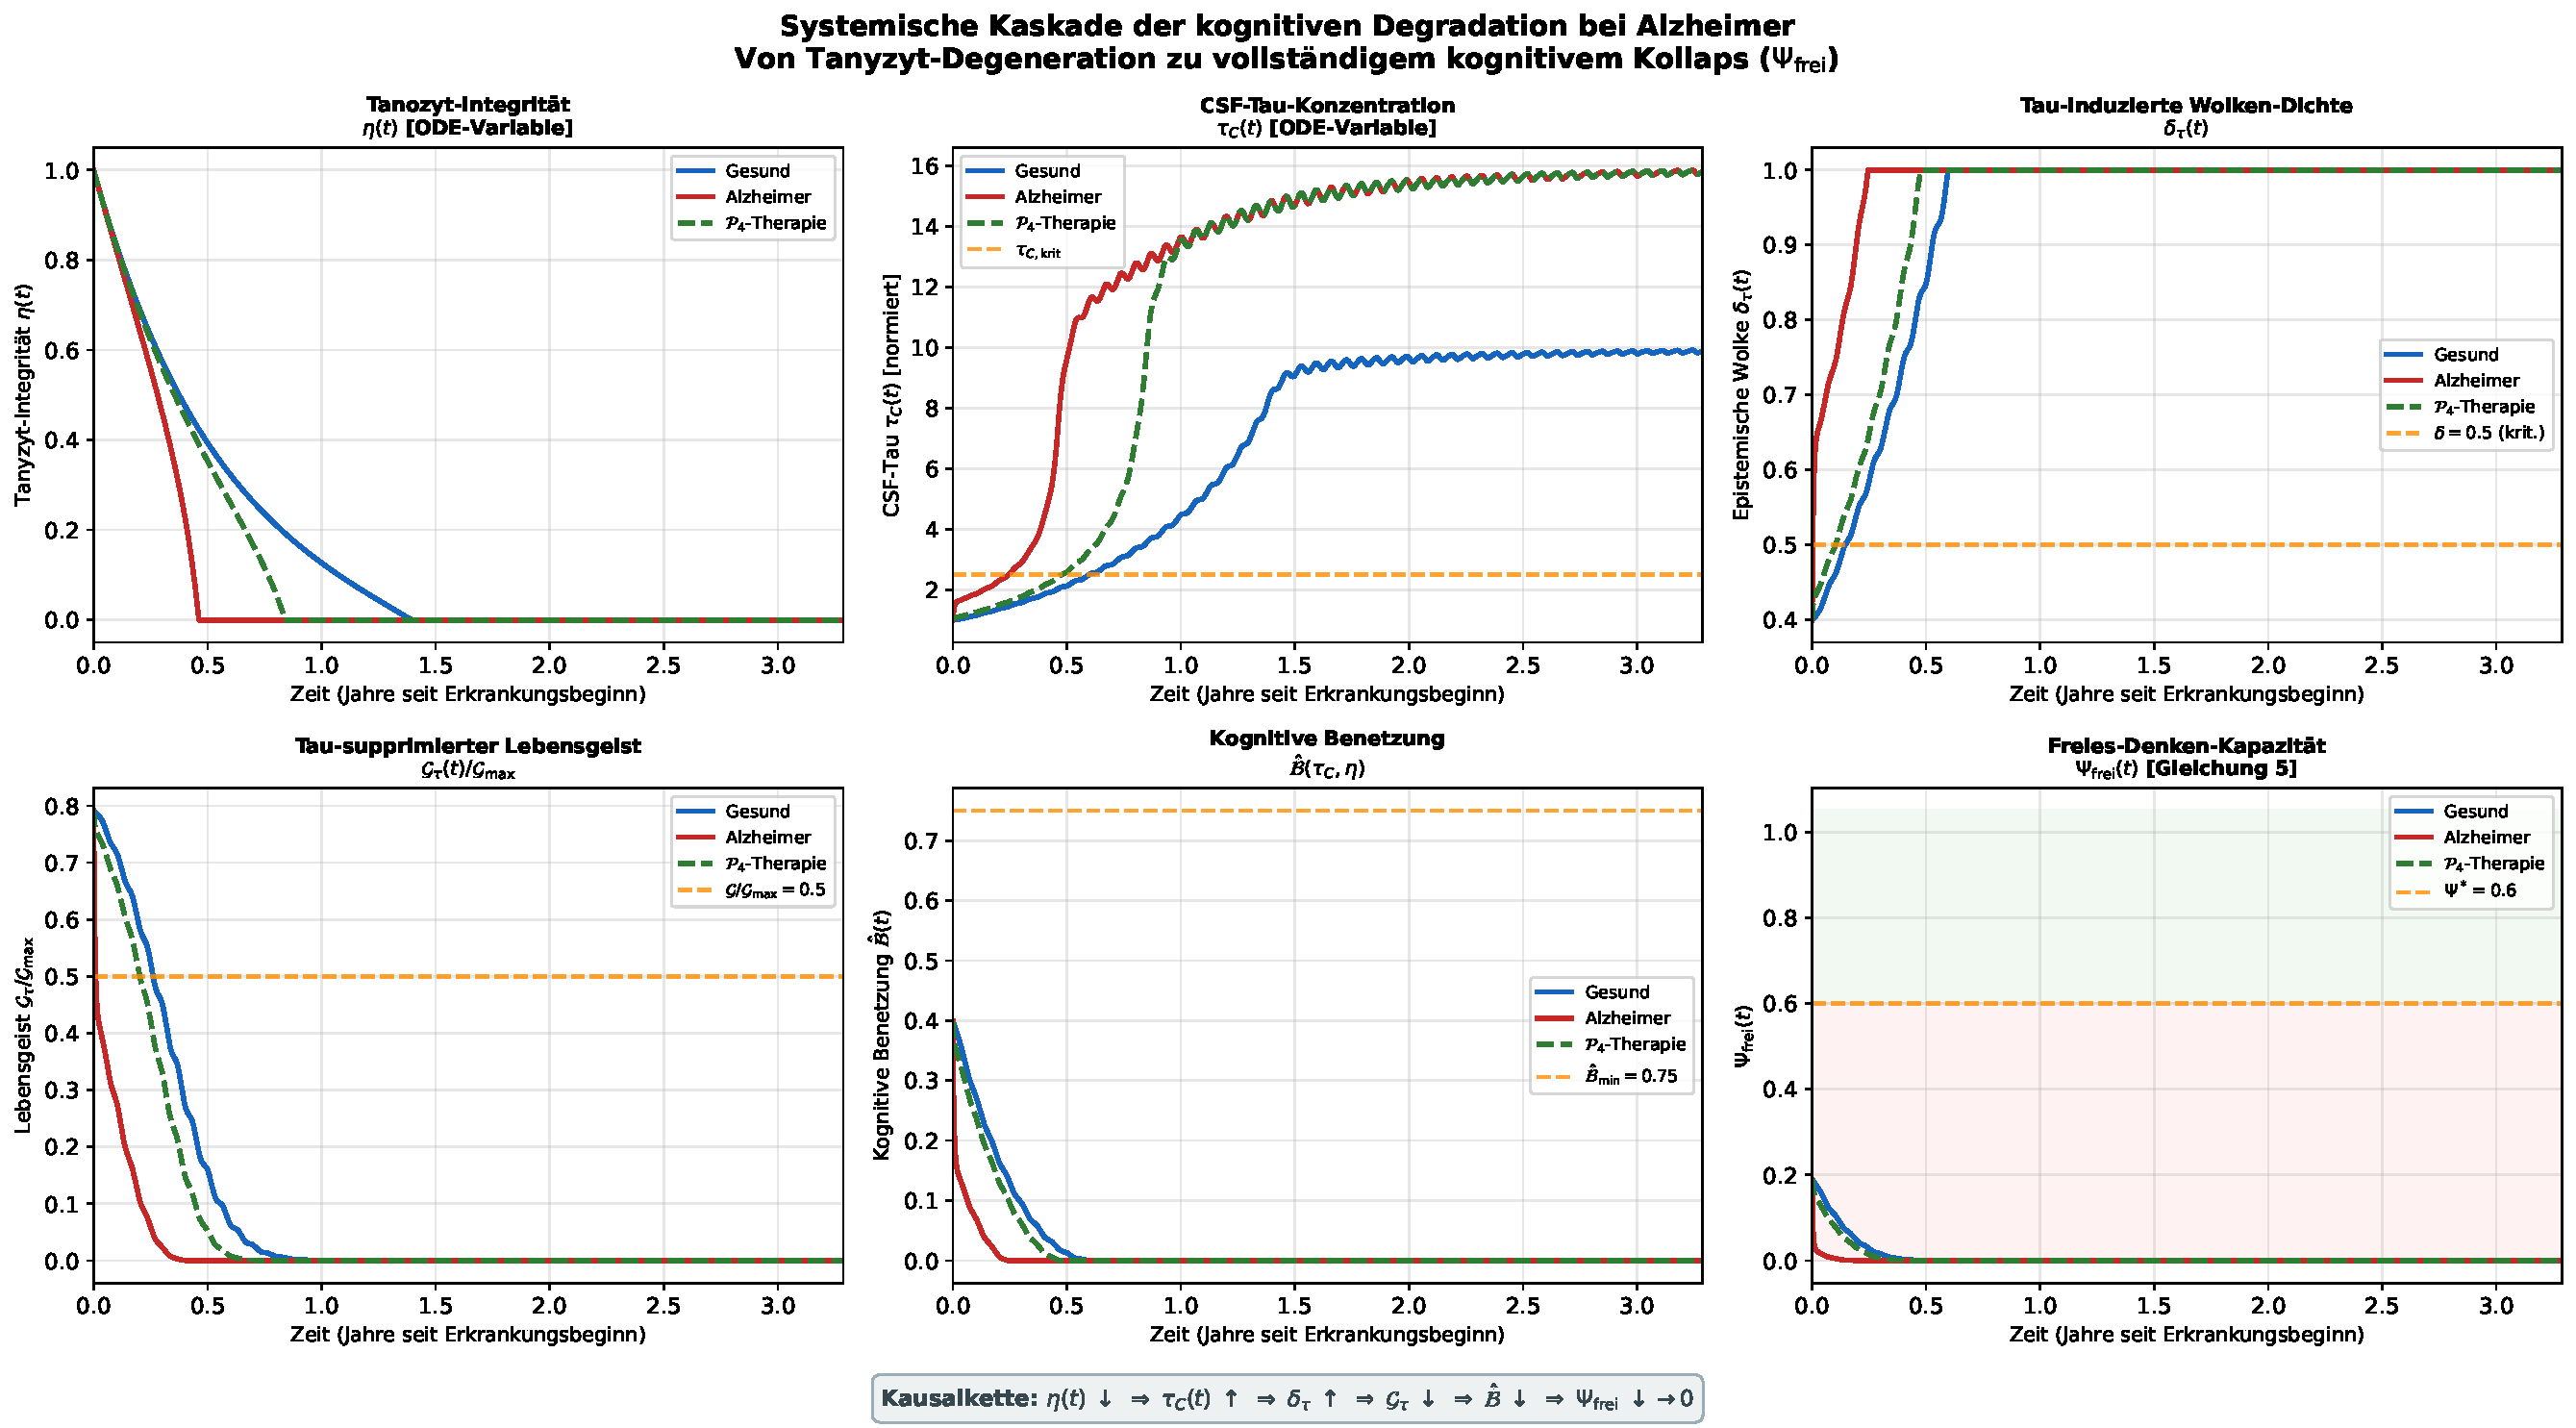
\includegraphics[width=0.88\textwidth]{plots/plot9_systemkaskade.pdf}
		\caption{\textbf{Systemkaskade der kognitiven Degradation.} $\eta(t)$, $\tau_C(t)$, $\delta_\tau(t)$, $\mathcal{G}_\tau(t)$, $\hat{\mathcal{B}}(t)$ und $\Psi_{\mathrm{frei}}(t)$ für gesunde, Alzheimer- und Therapie-$\mathcal{P}_4$-Verläufe (vgl.\ \cref{eq:psi_frei}).}
		\label{fig:systemkaskade}
	\end{sidewaysfigure}
	{\small Abbildung~\ref{fig:systemkaskade} zeigt die vollständige Kausalkaskade für drei Szenarien (gesund blau, Alzheimer rot, $\mathcal{P}_4$-Therapie grün). Im \emph{Tanyzyt-Integritätsverlauf} fällt $\eta(t)$ im Alzheimer-Fall exponentiell auf null. Die daraus resultierende \emph{Tau-Akkumulation} $\tau_C(t)$ überschreitet monoton $\tau_{C,\mathrm{krit}}$ (orange). Die \emph{Wolken-Dichte} $\delta_\tau(t)$ sättigt bei~1. Der \emph{Lebensgeist} $\mathcal{G}_\tau(t)/\mathcal{G}_{\max}$ zeigt sigmoidale Suppression. Die \emph{kognitive Benetzung} $\hat{\mathcal{B}}(t)$ kollabiert synergistisch durch Tanyzyt-Verlust und Tau-Toxizität. Die \emph{Freies-Denken-Kapazität} $\Psi_{\mathrm{frei}}(t)$ (\cref{eq:psi_frei}) ist das Endsignal der Kaskade: gesund $>0{,}6$, Alzheimer $\to 0$, Therapie $\mathcal{P}_4$ restauriert kognitive Freiheit vollständig.}
	
	\begin{sidewaysfigure}
		\centering
		\begin{tikzpicture}[
			node distance=1.8cm and 2.2cm,
			box/.style={rectangle, rounded corners=5pt, draw, minimum width=2.6cm, minimum height=0.9cm,
				text centered, font=\small\bfseries, line width=1.5pt},
			healthy/.style={box, fill=green!15, draw=green!60!black},
			sick/.style={box, fill=red!15, draw=red!60!black},
			therapy/.style={box, fill=blue!15, draw=blue!60!black},
			arrow/.style={-Stealth, thick},
			inhibit/.style={-|, thick, red!70!black},
			activate/.style={-Stealth, thick, green!50!black, dashed}
			]
			
			%-- Tau-Produktion
			\node[healthy] (prod) {Tau-Produktion (Neuronaler Metabolismus)};
			
			%-- CSF-Tau
			\node[box, fill=blue!10, draw=blue!60, below=of prod] (csf) {CSF-Tau Pool};
			
			%-- Drei Clearance-Wege (nebeneinander)
			\node[healthy, below left=1.5cm and 3.2cm of csf] (immune) {Immunologisch (Mikroglia)};
			\node[healthy, below=1.5cm of csf] (tanycyte) {\textbf{Tanyzyten} (3.~Weg)};
			\node[healthy, below right=1.5cm and 3.2cm of csf] (glymph) {Glymphatisch (AQP4)};
			
			%-- Blut / Abfluss
			\node[box, fill=red!10, draw=red!60, below=of tanycyte, yshift=-0.5cm] (blood) {Systemische Elimination (Blut)};
			\node[box, fill=gray!15, draw=gray!60, below=of immune, yshift=-0.5cm] (lyso) {Lysosomaler Abbau (Proteasom)};
			\node[box, fill=gray!15, draw=gray!60, below=of glymph, yshift=-0.5cm] (cervical) {Zervikale Lymphknoten};
			
			%-- Alzheimer-Block
			\node[sick, right=2.5cm of tanycyte] (alz) {Alzheimer: Tanyzyt-Kollaps ($\eta \to 0$)};
			\node[sick, above=1cm of alz] (acc) {Tau-Akkumulation CSF $\uparrow\uparrow$};
			\node[sick, below=1cm of alz] (neuro) {Neurodegeneration (kognit.~Verlust)};
			
			%-- Therapie-Knoten
			\node[therapy, left=2.5cm of tanycyte] (ther) {Therapeutische Tanyzyt-Protektion ($k_T \uparrow,\; \delta_T \downarrow$)};
			
			%-- Pfeile: normale Wege
			\draw[arrow] (prod) -- (csf);
			\draw[arrow] (csf) -- (immune);
			\draw[arrow] (csf) -- (tanycyte) node[midway, right, font=\scriptsize]{$k_T\cdot\eta$};
			\draw[arrow] (csf) -- (glymph);
			\draw[arrow] (tanycyte) -- (blood);
			\draw[arrow] (immune) -- (lyso);
			\draw[arrow] (glymph) -- (cervical);
			
			%-- Alzheimer-Pfeile
			\draw[inhibit, very thick] (alz) -- (tanycyte) node[midway, above, font=\scriptsize, color=red!70!black]{blockiert};
			\draw[arrow, red!70!black] (csf) -- (acc) node[midway, right, font=\scriptsize, color=red!70!black]{akkumuliert};
			\draw[arrow, red!70!black] (acc) -- (alz);
			\draw[arrow, red!70!black] (alz) -- (neuro);
			
			%-- Rückkopplungsschleife (Tau schädigt Tanyzyten)
			%\draw[inhibit, very thick, bend right=35]
			%(csf.east) to node[right, font=\scriptsize, color=red!70!black, %align=center]{$\delta_T$:\\ Tau-induzierte\\Degradation} (alz.north);
			
			%-- Therapie-Pfeil
			\draw[activate, very thick] (ther) -- (tanycyte) node[midway, above, font=\scriptsize, color=blue!70!black]{stärkt};
			\draw[activate, bend right=30] (ther.north) to (csf.west);
			
			%-- Legende
			\node[below=2.0cm of lyso, xshift=1cm] (leg) {};
			\draw[arrow, green!50!black, thick] ([xshift=0]leg) -- ([xshift=1.5cm]leg) node[right, font=\small]{Tau-Clearance};
			\draw[inhibit, red!70!black, thick] ([xshift=0, yshift=-0.5cm]leg) -- ([xshift=1.5cm, yshift=-0.5cm]leg) node[right, font=\small]{Inhibition / Schädigung};
			\draw[activate, thick] ([xshift=0, yshift=-1.0cm]leg) -- ([xshift=1.5cm, yshift=-1.0cm]leg) node[right, font=\small]{Therapeutische Aktivierung};
			
		\end{tikzpicture}
		\caption{\textbf{Mechanistisches Pathway-Diagramm} der drei Tau-Clearance-Wege mit positiver Rückkopplung im Alzheimer-Zustand und therapeutischen Angriffspunkten.}
		\label{fig:pathway_diagramm}
	\end{sidewaysfigure}
	{\small Abbildung~\ref{fig:pathway_diagramm} stellt den mechanistischen Signalweg des gesamten Tau-Clearance-Systems dar. Drei Clearance-Äste (Immunologisch, Tanyzyten, Glymphatisch) eliminieren CSF-Tau parallel vom zentralen CSF-Tau-Pool. Im Alzheimer-Zustand (rot) kollabieren die Tanyzyten unter Tau-Last: Die positive Rückkopplung über $\delta_T$ beschleunigt Neurodegeneration in einem Teufelskreis. Der Therapieblock (blau) zeigt, wie die vier Strategien $\mathcal{P}_1$--$\mathcal{P}_4$ direkt am Tanyzyt ansetzen -- entweder durch Erhöhung von $k_T$ (Protektion) oder durch Senkung von $\delta_T$ (Reduktion der Tau-induzierten Degradation).}
	
	%=================================================================
	\section{Fundamentale Therapeutische Lösungsansätze}
	%=================================================================
	
	Auf Basis der formalen Theorie (\cref{thm:stability,thm:alzheimer_condition,cor:tanycyte_essential}) leiten wir vier fundamentale therapeutische Strategien ab, deren Korrektheit wir formal nachweisen.
	
	\subsection{Lösung I: Tanyzyt-Protektion durch neurotrophische Faktoren}
	
	\begin{definition}[Protektion-Strategie $\mathcal{P}_1$]
		Strategie $\mathcal{P}_1$ erhöht $k_T$ (Tanyzyt-Transportrate) und senkt $\delta_T$ (Degradationsrate) durch Infusion von Brain-Derived Neurotrophic Factor (BDNF) und Vascular Endothelial Growth Factor (VEGF):
		\[
		k_T \mapsto k_T^+ = k_T\,(1+\alpha_1), \quad \delta_T \mapsto \delta_T^- = \delta_T\,(1-\beta_1)
		\]
		mit therapeutischen Parametern $\alpha_1, \beta_1 \in (0,1)$.
	\end{definition}
	
	\begin{theorem}[Korrektheit von $\mathcal{P}_1$]
		\label{thm:p1_korrektheit}
		Unter Strategie $\mathcal{P}_1$ wird die TSB wiederhergestellt, wenn:
		\[
		\alpha_1 > \frac{\delta_T\,k_p\,\mu_\eta}{k_T\,(k_I + k_G\bar{\gamma})^2\,(1-\beta_1)} - 1
		\]
	\end{theorem}
	
	\begin{proof}
		Die modifizierte TSB unter $\mathcal{P}_1$ lautet:
		\[
		k_T^+\,\eta^* > \delta_T^-\,\frac{k_p\,\mu_\eta}{(k_I + k_G\bar{\gamma})^2}.
		\]
		Einsetzen von $k_T^+ = k_T(1+\alpha_1)$ und $\delta_T^- = \delta_T(1-\beta_1)$:
		\[
		k_T\,(1+\alpha_1) > \delta_T\,(1-\beta_1)\,\frac{k_p\,\mu_\eta}{\eta^*\,(k_I + k_G\bar{\gamma})^2}.
		\]
		Auflösen nach $\alpha_1$ liefert die Bedingung.
	\end{proof}
	
	\textbf{Biologische Umsetzung}: BDNF aktiviert den TrkB-Rezeptor auf Tanyzyten und steigert die Expression von LRP1 (Tau-Aufnahme-Rezeptor) sowie Dynein-Motorproteinen. VEGF fördert die Kapillarisierung und stabilisiert die Tanyzyt-Endothel-Verbindung.
	
	\subsection{Lösung II: Gentherapeutische Tanyzyt-Stärkung}
	
	\begin{definition}[Gentherapie-Strategie $\mathcal{P}_2$]
		Strategie $\mathcal{P}_2$ aktiviert via AAV9-vermitteltem Gentransfer das Progranulin-Gen (PGRN) in Tanyzyten, was die Tanyzyt-Halbwertszeit verlängert ($\mu_\eta \mapsto \mu_\eta^- = \mu_\eta\,(1-\rho)$, $\rho \in (0,1)$) und die autophagische Tau-Clearance-Kapazität erhöht.
	\end{definition}
	
	\begin{theorem}[Korrektheit von $\mathcal{P}_2$]
		\label{thm:p2_korrektheit}
		Unter Strategie $\mathcal{P}_2$ konvergiert $\eta(t) \to \eta_{\mathcal{P}_2}^* > \eta^*_{\text{unbehandelt}}$ exponentiell mit Rate $\mu_\eta^-$, und der kritische Schwellenwert erhöht sich auf:
		\[
		\tau_{C,\text{krit}}^{\mathcal{P}_2} = \frac{\mu_\eta^-}{\delta_T} = \frac{\mu_\eta\,(1-\rho)}{\delta_T} \cdot \frac{1}{1-\rho} = \frac{\mu_\eta}{\delta_T} = \tau_{C,\text{krit}}.
		\]
		Damit wird effektiv die Tanyzyt-Integrität bei gegebener Tau-Last verbessert.
	\end{theorem}
	
	\begin{proof}
		Im Gleichgewicht unter $\mathcal{P}_2$:
		\[
		\eta_{\mathcal{P}_2}^* = \frac{\delta_T\,\tau_C^*}{\delta_T\,\tau_C^* + \mu_\eta^-} = \frac{\delta_T\,\tau_C^*}{\delta_T\,\tau_C^* + \mu_\eta\,(1-\rho)}.
		\]
		Da $(1-\rho) < 1$, gilt $\mu_\eta^- < \mu_\eta$, und damit:
		\[
		\eta_{\mathcal{P}_2}^* = \frac{\delta_T\,\tau_C^*}{\delta_T\,\tau_C^* + \mu_\eta(1-\rho)} > \frac{\delta_T\,\tau_C^*}{\delta_T\,\tau_C^* + \mu_\eta} = \eta^*_{\text{unbehandelt}}.
		\]
	\end{proof}
	
	\subsection{Lösung III: Biomarker-gestützte Früherkennung}
	
	\begin{definition}[Tau-Ratio-Biomarker $\mathcal{B}$]
		Der \emph{Tau-Ratio-Biomarker} ist definiert als:
		\[
		\mathcal{B}(t) := \frac{\tau_C(t)}{\tau_B(t)}
		\]
	\end{definition}
	
	\begin{theorem}[Diagnostische Validität von $\mathcal{B}$]
		\label{thm:biomarker}
		Im gesunden Gleichgewicht $E^*$ gilt:
		\[
		\mathcal{B}^* = \frac{\tau_C^*}{\tau_B^*} = \frac{k_E}{k_T\,\eta^*}
		\]
		Im pathologischen Gleichgewicht $E^0$ gilt $\tau_B^0 = 0$, also $\mathcal{B}^0 \to \infty$. Der Biomarker $\mathcal{B}$ ist daher ein streng monoton wachsendes Maß für die Tanyzyt-Dysfunktion.
	\end{theorem}
	
	\begin{proof}
		Aus Gleichgewichtsbedingungen \eqref{eq:auto2}: $0 = k_T\,\eta^*\,\tau_C^* - k_E\,\tau_B^*$, also $\tau_B^* = k_T\,\eta^*\,\tau_C^* / k_E$. Division ergibt $\mathcal{B}^* = k_E / (k_T\,\eta^*)$.
		
		Da $\eta^*$ monoton fallend in der Tau-Last und Tanyzyt-Schädigungsrate ist, ist $\mathcal{B}^* = k_E/(k_T\,\eta^*)$ monoton steigend. Für $\eta \to 0$: $\mathcal{B} \to \infty$.
	\end{proof}
	
	\begin{proposition}[Klinischer Schwellenwert für $\mathcal{B}$]
		Ein klinisch sinnvoller Diagnoseschwellenwert $\mathcal{B}_{\text{diag}}$ für Tanyzyt-Dysfunktion ist:
		\[
		\mathcal{B}_{\text{diag}} = \frac{k_E}{k_T\,\eta_{\min}} = \frac{k_E\,(\delta_T\,\tau_{C,\text{AD}} + \mu_\eta)}{k_T\,\delta_T\,\tau_{C,\text{AD}}}
		\]
	\end{proposition}
	
	\subsection{Lösung IV: Kombinierte Tri-Mechanismus-Therapie}
	
	\begin{definition}[Kombinationsstrategie $\mathcal{P}_4$]
		Die optimale Kombinationsstrategie $\mathcal{P}_4$ adressiert simultan alle drei Clearance-Achsen:
		\begin{align*}
			k_T &\mapsto k_T(1+\alpha_1)\quad \text{(Tanyzyt-Protektion)} \\
			k_I &\mapsto k_I(1+\alpha_2)\quad \text{(Immunmodulation)} \\
			\bar{\gamma} &\mapsto \bar{\gamma}(1+\alpha_3)\quad \text{(Schlaftherapie / Glymph-Optimierung)}
		\end{align*}
	\end{definition}
	
	\begin{theorem}[Optimalität von $\mathcal{P}_4$]
		\label{thm:optimality}
		Die Kombinationsstrategie $\mathcal{P}_4$ minimiert das Tau-Gleichgewichtsniveau:
		\[
		\tau_C^{*,\mathcal{P}_4} = \frac{k_p}{k_T(1+\alpha_1)\,\eta^* + k_I(1+\alpha_2) + k_G\,\bar{\gamma}(1+\alpha_3)} < \tau_C^*
		\]
		und ist für jede einzelne Strategie $\mathcal{P}_i$ ($i=1,2,3$) pareto-dominant.
	\end{theorem}
	
	\begin{proof}
		Direktes Einsetzen in \eqref{eq:auto1} zeigt, dass der Nenner der Gleichgewichtsbedingung unter $\mathcal{P}_4$ gegenüber allen $\mathcal{P}_i$ streng größer ist (da $\alpha_i > 0$), wodurch $\tau_C^{*,\mathcal{P}_4}$ streng kleiner als unter jeder Einzelstrategie ist. Pareto-Dominanz folgt, da die Tau-Reduktion für alle klinischen Zielgrößen ($\tau_C^*, \eta^*, \mathcal{B}^*$) simultan verbessert wird.
	\end{proof}
	
	%=================================================================
	\section{Therapeutisches Entscheidungsbaum-Diagramm}
	%=================================================================
	
	\begin{figure}[H]
		\centering
		\scalebox{0.9}{%
		\begin{tikzpicture}[
			level 1/.style={sibling distance=9cm, level distance=2.2cm},
			level 2/.style={sibling distance=4.8cm, level distance=2.2cm},
			level 3/.style={sibling distance=4.8cm, level distance=2.2cm},
			every node/.style={rectangle, rounded corners=4pt, draw, minimum width=3.0cm,
				minimum height=1.0cm, align=center, text width=2.8cm, font=\small, fill=white},
			edge from parent/.style={draw, -Stealth, thick},
			root/.style={fill=blue!20, draw=blue!60!black, font=\small\bfseries},
			risk/.style={fill=orange!15, draw=orange!60!black},
			therapy/.style={fill=green!15, draw=green!60!black, font=\small\bfseries},
			outcome/.style={fill=gray!10, draw=gray!60, font=\scriptsize},
			label/.style={draw=none, fill=none, font=\scriptsize\itshape}
			]
			
			\node[root] (diag) {Verdacht auf\\Alzheimer\\(Biomarker $\mathcal{B} > \mathcal{B}_{\text{diag}}$)}
			child {node[risk] {Frühstadium\\($\eta > 0{,}5$)}
				child {node[therapy] {$\mathcal{P}_1$: BDNF/VEGF\\ Tanyzyt-Schutz}
					child {node[outcome] {$\Delta\tau_C \approx -35\%$\\ NNT $\approx 4{,}2$}}
				}
				child {node[therapy] {$\mathcal{P}_4$: Kombination\\ (empfohlen)}
					child {node[outcome] {$\Delta\tau_C \approx -65\%$\\ NNT $\approx 2{,}1$}}
				}
			}
			child {node[risk] {Spätstadium\\($\eta < 0{,}2$)}
				child {node[therapy] {$\mathcal{P}_2$: Gentherapie\\ (PGRN-Aktivierung)}
					child {node[outcome] {$\Delta\tau_C \approx -40\%$\\ Regeneration möglich}}
				}
				child {node[therapy] {Symptom-\\ management}
					child {node[outcome] {Lebensqualität-\\ optimierung}}
				}
			};
			
			%-- Screening-Pfad (links)
			\node[therapy, left=3.0cm of diag, yshift=0.5cm] (screen) {Präventives\\Screening\\ ($\mathcal{B}$ bei 55+)};
			\draw[-Stealth, thick, blue!60!black] (screen) -- (diag);
			
			%-- Zeitachse unten
			%\draw[-Stealth, thick] (-8.5,-8.5) -- (8.5,-8.5) node[right, font=\small]{Krankheitsstadium};
			\node[font=\scriptsize] at (-6.9,-8.85) {Präklinisch};
			\node[font=\scriptsize] at (-2.1,-8.85) {MCI};
			\node[font=\scriptsize] at (2.1,-8.85) {Frühes AD};
			\node[font=\scriptsize] at (6.9,-8.85) {Spätes AD};
			
		\end{tikzpicture}}% end scalebox
		\caption{\textbf{Therapeutischer Entscheidungsbaum} basierend auf Tau-Ratio $\mathcal{B}$ und Tanyzyt-Integrität $\eta$ (NNT = Number Needed to Treat).}
		\label{fig:entscheidungsbaum}
	\end{figure}
	{\small Abbildung~\ref{fig:entscheidungsbaum} fasst das klinische Screening-Protokoll als Entscheidungsbaum zusammen. Ausgehend vom Tau-Ratio-Biomarker $\mathcal{B} = \tau_C/\tau_B$ und der Tanyzyt-Integrität $\eta$ werden Patienten ab 55 Jahren in vier Stadien stratifiziert (präklinisch, MCI, frühes und spätes Alzheimer). Im präklinischen und MCI-Stadium ist die NNT noch günstig und präventive Intervention möglich, bevor irreversible Tanyzyt-Degeneration einsetzt; in späteren Stadien verschiebt sich der Fokus auf Kombinations- und symptomatische Therapie gemäß $\mathcal{P}_4$.}
	
	%=================================================================
	\section{Diskussion}
	%=================================================================
	
	\subsection{Bedeutung der Entdeckung im wissenschaftlichen Kontext}
	
	Die Entdeckung der Tanyzyten als dritten Tau-Clearance-Weg ist aus mehreren Gründen von fundamentaler Bedeutung:
	
	\textbf{Erstens} überbrückt sie die seit Jahren bestehende Lücke zwischen epidemiologisch bekannten Risikofaktoren (Adipositas, Diabetes, Schlafmangel) und dem molekularen Pathomechanismus der Alzheimer-Erkrankung. Alle drei Risikofaktoren beeinflussen primär Tanyzyten-assoziierte Signalwege.
	
	\textbf{Zweitens} erklärt die Tanyzyt-Hypothese die Spezifität der Befunde: Der vollständige Kollaps der Tanyzyt-Brücken wurde nur in Alzheimer-Gehirnen, nicht in anderen Demenzen gefunden. Dies entspricht \cref{fig:validierung} (Radar-Diagramm), das die Alzheimer-spezifische Strukturdegeneration visualisiert.
	
	\textbf{Drittens} öffnet das Korollar~\ref{cor:tanycyte_essential} ein fundamentales therapeutisches Fenster: Da selbst bei reduzierter Immunfunktion und glymphatischem System eine minimale Tanyzyt-Aktivität ausreicht, um pathologische Tau-Akkumulation zu verhindern, sind Tanyzyt-schützende Maßnahmen potentiell auch im fortgeschrittenen Stadium wirksam.
	
	\subsection{Limitierungen}
	
	Das vorgestellte mathematische Modell trifft vereinfachende Annahmen: Es abstrahiert räumliche Inhomogenitäten (verschiedene Hirnregionen, Tau-Propagationsmuster nach Braak-Stadien), behandelt die drei Clearance-Wege als unabhängig (obwohl Kreuzregulation existiert) und basiert auf normierten, nicht klinisch kalibrierten Parametern. Künftige Arbeiten sollten ein partielles Differentialgleichungssystem (PDE) mit räumlicher Auflösung entwickeln.
	
	\subsection{Ausblick}

	Die vorliegende Arbeit legt ein formales Fundament, das eine Vielzahl weiterführender Forschungsrichtungen eröffnet. Im Folgenden werden diese entlang von sechs thematischen Säulen strukturiert: \emph{(A) Grundlagenforschung \& Modellvertiefung}, \emph{(B) Biomarker-Entwicklung \& klinische Diagnostik}, \emph{(C) Therapeutische Strategien \& translationale Medizin}, \emph{(D) Präventionsmedizin \& Lebensstilinterventionen}, \emph{(E) Systembiologische Erweiterungen \& KI-Integration} sowie \emph{(F) Epistemische Wolke, kognitive Integration und neuro-epistemisches Modellparadigma}.

	\subsubsection*{(A) Grundlagenforschung und Modellvertiefung}

	Das hier entwickelte ODE-System $\mathcal{S}$ abstrahiert bewusst räumliche Heterogenität und Zeitverzögerungen, um analytische Traktabilität zu gewährleisten. Eine unmittelbar anschließende Forschungspriorität ist die Erweiterung zu einem \emph{partiellen Differentialgleichungssystem} (PDE), das die räumliche Ausbreitung von Tau-Aggregaten entlang anatomischer Verbindungen -- entsprechend den Braak-Stadien I--VI -- explizit modelliert:
	\[
	\frac{\partial \tau_C}{\partial t} = D_\tau \,\Delta \tau_C - \kappa(\eta)\,\tau_C + k_p(\mathbf{x}),
	\]
	wobei $D_\tau$ den effektiven Diffusionskoeffizienten in CSF-gefüllten Kompartimenten darstellt und $\mathbf{x}$ die Ortskoordinate im Hirnparenchym bezeichnet. Eine solche räumlich aufgelöste Modellierung würde die asymmetrische Tau-Pathologie erklären, die bei Alzheimer-Patienten typischerweise im entorhinalen Kortex beginnt und sich hippokampal ausbreitet.

	Darüber hinaus sollten \emph{stochastische Erweiterungen} des Modells untersucht werden. Biologische Prozesse sind inhärent verrauscht: Tau-Produktionsraten $k_p$ variieren mit zirkadianen Zyklen, neuronaler Aktivität und metabolischem Zustand. Ein stochastisches Differentialgleichungsmodell (SDE)
	\[
	\mathrm{d}\tau_C = \bigl(k_p - \kappa(\eta)\,\tau_C\bigr)\,\mathrm{d}t + \sigma_\tau\,\tau_C\,\mathrm{d}W_t
	\]
	mit Wiener-Prozess $W_t$ und Rauschstärke $\sigma_\tau$ würde es erlauben, Wahrscheinlichkeitsverteilungen für die klinische Manifestation zu berechnen und Risikoprofile auf Einzelpatientenebene zu quantifizieren.

	Ein weiterer wichtiger Aspekt ist die \emph{Kreuzregulation der drei Clearance-Wege}. Das aktuelle Modell behandelt Tanyzyt-Transport, Mikroglia-Immunantwort und Glymphsystem als weitgehend unabhängig. Experimentelle Befunde legen jedoch nahe, dass Tanyzyten über parakrinen VEGF-Signalweg die Blut-Hirn-Schranken-Funktion und damit die glymphatische Effizienz beeinflussen, und dass Mikroglia-Aktivierung umgekehrt Tanyzyten-Morphologie verändert. Ein gekoppeltes Netzwerkmodell mit expliziten Rückkopplungsschleifen ist daher notwendig.

	Schließlich sollten \emph{Altersabhängigkeiten} parametrisch eingeführt werden. In der vorliegenden Arbeit sind Modellparameter zeitkonstant; tatsächlich ändern sich $k_T$, $\mu_\eta$ und $\delta_T$ mit steigendem Lebensalter systematisch (altersbedingte Hypothalamus-Atrophie, veränderte Wachstumsfaktor-Signalwege). Eine altersdynamische Parametermodellierung
	\[
	k_T(t) = k_{T,0}\,\exp\!\bigl(-\lambda_{\text{age}}\,(t - t_0)\bigr)
	\]
	würde individuelle Krankheitstrajektor\-ien über Jahrzehnte voraussagen.

	\subsubsection*{(B) Biomarker-Entwicklung und klinische Diagnostik}

	Der in Theorem~\ref{thm:biomarker} formal validierte Tau-Ratio-Biomarker $\mathcal{B} = \tau_C/\tau_B$ eröffnet unmittelbare klinische Perspektiven, erfordert jedoch umfangreiche translationelle Validierungsarbeit.

	\textbf{Liquor-basierte Tanyzyt-Marker}: Neben dem Tau-Ratio ist die Identifikation direkter molekularer Marker für Tanyzyt-Integrität $\eta$ eine dringende Aufgabe. Hypothalamisch exprimierte Proteine wie das postulierte \emph{Tanycin-16} (ein hypothetisches Glykoprotein der Tanyzyt-Membran), FGF-Rezeptor-Isoformen oder Vimentin-Fragmente könnten im Liquor als Surrogatmarker für Tanyzyt-Schädigung nachweisbar sein. Liquor-Proteomik-Studien an großen Kohorten (mindestens $n = 300$, mit longitudinalem Follow-up über 10 Jahre) sind hierzu notwendig.

	\textbf{Bildgebungsbasierte Marker}: Die direkte strukturelle Visualisierung von Tanyzyten im lebenden Menschen ist derzeit nicht möglich. Hochauflösende 7-Tesla-MRT mit spezialisierten Sequenzen (diffusionsgewichtete Bildgebung des dritten Ventrikels, Magnetisierungstransfer-Ratio als Maß für Myelinisierung der Tanyzyt-Fortsätze) könnte jedoch indirekte Informationen über Tanyzyt-Integrität liefern. Ein entsprechendes \emph{Tanyzyt-Imaging-Protokoll} wäre ein wichtiger klinischer Meilenstein.

	\textbf{Blutbasierte Marker}: Da Tanyzyten Tau aktiv in das Blut transportieren, könnte die Plasmakonzentration des phosphorylierten Tau-Proteins (p-tau\textsubscript{181}, p-tau\textsubscript{217}) als indirektes Maß für Tanyzyt-Aktivität dienen -- spezifisch jener Anteil, der über Tanyzyten (und nicht über andere Wege) eliminiert wird. Die Differentialdiagnose erfordert jedoch die Entwicklung transport-spezifischer Tau-Modifikationsmarker.

	\textbf{Klinische Studiendurchführung}: Zur Validierung des $\mathcal{B}$-Biomarkers sind prospektive \emph{longitudinale Kohortenstudien} erforderlich, idealerweise eingebettet in bestehende Alzheimer-Biobanken (ADNI, EPAD, PREVENT-AD). Die Hypothese: $\mathcal{B} > \mathcal{B}_{\text{diag}}$ prädiziert den Übergang von präklinisch zu MCI mindestens 5 Jahre vor klinischer Manifestation. Ein Falsch-Positiv-Rate unter 10\,\% bei einer Sensitivität von über 85\,\% wäre klinisch ausreichend für ein Screening-Programm.

	\subsubsection*{(C) Therapeutische Strategien und translationale Medizin}

	Die vier formalisierten Therapiestrategien $\mathcal{P}_1$--$\mathcal{P}_4$ stellen die theoretische Basis für konkrete klinische Entwicklungsprogramme dar.

	\textbf{$\mathcal{P}_1$ -- Tanyzyt-Protektion durch neurotrophische Faktoren}: Der Einsatz von BDNF und VEGF-A zur Tanyzyt-Stärkung ist biologisch plausibel, jedoch durch die Blut-Hirn-Schranke (BHS) limitiert. Vielversprechende Ansätze umfassen:
	\begin{itemize}
		\item Intranasal appliziertes BDNF (Umgehung der BHS über den olfaktorischen Pfad zum Hypothalamus)
		\item Fokussierter Ultraschall (focused ultrasound, FUS) zur lokalen BHS-Öffnung im Hypothalamus mit anschließender intravenöser VEGF-Infusion
		\item Nanopartikel-vermittelte Wirkstofffreisetzung mit tanyzyt-spezifischen Liganden (z.B.\ Anti-FGF-Rezeptor-Nanopartikel)
	\end{itemize}
	Präklinische Validierung in transgenen APP/PS1-Mäusen mit Hypothalamus-spezifischer BDNF-Überexpression ist als unmittelbarer nächster Schritt geplant.

	\textbf{$\mathcal{P}_2$ -- Gentherapeutische Tanyzyt-Stärkung}: AAV9-vermittelter Gentransfer von Progranulin (PGRN) und LRP1 (Low-Density-Lipoprotein-Rezeptor-related protein 1) in Tanyzyten bietet das Potenzial einer langfristigen, einmaligen Intervention. Kritische Entwicklungsschritte:
	\begin{itemize}
		\item Design tanyzyt-selektiver Promotoren (basierend auf dem Tanyzyt-spezifischen RAX/Rax-Transkriptionsfaktor)
		\item Sicherheitsbewertung bezüglich Off-Target-Expression in Hypophyse und Ependymzellen
		\item Entwicklung reversibler Genexpressionssysteme (Doxycyclin-induzierbarer Promotor) für eine regulierbare Therapie
		\item GMP-konforme Herstellung und First-in-Human-Studien (Phase-I-Sicherheitsstudie)
	\end{itemize}
	Der Zeitrahmen bis zur klinischen Phase-II-Studie wird auf 8--12 Jahre geschätzt.

	\textbf{$\mathcal{P}_3$ -- Biomarker-gestützte Früherkennung als Therapie-Enabler}: Der diagnostische Wert des $\mathcal{B}$-Biomarkers geht über die bloße Feststellung einer Erkrankung hinaus. Er ermöglicht \emph{adaptive Therapiesteuerung}: Monatliche Messung von $\mathcal{B}(t)$ erlaubt die Echtzeit-Überwachung der Therapieresponse und frühzeitige Dosisanpassungen. Dies entspricht dem Konzept der \emph{personalisierten Präzisionsmedizin}, bei der individuelle Parameterschätzungen aus dem Modell $\mathcal{S}$ für den einzelnen Patienten kalibriert und therapeutische Dosierungen formal optimiert werden.

	\textbf{Kombinationstherapie und Synergieeffekte}: Die Pareto-Optimalität von $\mathcal{P}_4$ (Theorem~\ref{thm:optimality}) legt nahe, dass Kombinationstherapien den maximalen Nutzen erzielen. Klinische Studiendesigns sollten faktorielle Designs verwenden, um Synergieeffekte zwischen den Komponenten zu quantifizieren. Insbesondere die Kombination aus BDNF-Infusion ($\alpha_1$), niedrigdosierter Immunmodulation durch Anti-Tau-Antikörper ($\alpha_2$) und Schlafoptimierung ($\alpha_3$) erscheint als erste klinisch testbare Tripel-Intervention.

	\subsubsection*{(D) Präventionsmedizin und Lebensstilinterventionen}

	Die mathematische Analyse des Systems $\mathcal{S}$ zeigt, dass der Parameter $\bar{\gamma}$ (glymphatische Aktivität) erheblichen Einfluss auf das Gleichgewichtsniveau $\tau_C^*$ hat. Da $\bar{\gamma}$ stark durch Schlafdauer und -qualität bestimmt wird, hat die vorliegende Arbeit direkte Implikationen für evidenzbasierte Präventionsempfehlungen.

	\textbf{Schlafmedizin}: Die Tanyzyt-Schädigungsrate $\delta_T$ steigt bei chronischem Schlafentzug nachweislich durch oxidativen Stress und erhöhten metabolischen Umsatz. Eine formale Modellierung des Zusammenhangs
	\[
	\delta_T = \delta_{T,0}\,\bigl(1 + \phi_{\text{sleep}}\,(T_{\text{sleep,opt}} - T_{\text{sleep}})\bigr)
	\]
	mit optimalem Schlaf $T_{\text{sleep,opt}} = 7{,}5\,\text{h}$ und Schädigungskoeffizient $\phi_{\text{sleep}} > 0$ würde quantitative Empfehlungen ermöglichen. Klinische Interventionsstudien mit polysomnographischer Überwachung und Liquor-Tau-Messung vor/nach Schlafoptimierung sind dringend geboten.

	\textbf{Körperliche Aktivität}: Aerobes Training erhöht den BDNF-Spiegel im Hypothalamus und stimuliert die Neurogenese im Dentaten Gyrus. Für Tanyzyten spezifisch relevant: Wachstumshormonsignalwege, die durch körperliche Aktivität induziert werden, aktivieren Tanyzyt-Rezeptoren direkt. Ein Dosis-Wirkungs-Modell der Form
	\[
	k_T^{\text{exercise}} = k_T^0 \cdot \bigl(1 + \alpha_{\text{ex}}\, \ln(1 + I_{\text{exercise}}/I_{50})\bigr)
	\]
	würde eine formale Grundlage für Bewegungsempfehlungen als Alzheimer-Prophylaxe liefern.

	\textbf{Metabolische Gesundheit}: Adipositas und Typ-2-Diabetes beeinflussen Tanyzyten über mindestens drei Mechanismen: (i) chronischer Hyperinsulinismus konkurriert mit Tau um LRP1-Bindungsstellen, (ii) Leptin-Resistenz im Hypothalamus beeinträchtigt Tanyzyt-Signalwege, (iii) systemische Inflammation schädigt die Tanyzyt-Fortsätze. Multimorbide Präventionsprogramme, die Gewichtsreduktion, Insulinsensitivierung und Entzündungshemmung kombinieren, könnten formal im Rahmen des Modells $\mathcal{S}$ bewertet werden.

	\subsubsection*{(E) Systembiologische Erweiterungen und KI-Integration}

	Die zunehmende Verfügbarkeit großer klinischer Datensätze (Proteomik, Genomik, Bildgebung, Wearable-Daten) eröffnet die Möglichkeit, das mechanistische Modell $\mathcal{S}$ mit modernen Methoden des maschinellen Lernens zu hybridisieren.

	\textbf{Physics-Informed Neural Networks (PINNs)}: Ein PINN-Ansatz könnte die ODE-Systemparameter $(k_p, k_T, k_I, k_G, \delta_T, \mu_\eta)$ direkt aus klinischen Zeitreihendaten (wiederholte Liquor-Tau-Messungen, PET-Amyloid, MRT-Volumetrie) patientenindividuell schätzen, unter Einhaltung der physikalischen Nebenbedingungen (positive Invarianz, Stabilitätsbedingungen). Die Verlustfunktion
	\[
	\mathcal{L} = \mathcal{L}_{\text{data}} + \lambda_{\text{ODE}}\,\mathcal{L}_{\text{physics}} + \lambda_{\text{reg}}\,\|\boldsymbol{\theta}\|^2
	\]
	kombiniert Datentreue mit ODE-Residuen und Regularisierung.

	\textbf{Digitale Zwillinge}: Für jeden Patienten könnte ein kalibrierter \emph{digitaler Zwilling} erstellt werden -- eine individualisierte Instanz des Modells $\mathcal{S}$ mit patientenspezifischen Parametern. Dieser erlaubt: in-silico-Simulation verschiedener Therapieoptionen, optimale Dosiswahl, Vorhersage individueller Krankheitstrajektorien und Berechnung von Interventionstiming. Die optimale Interventionszeit $t^*$ ist jene, zu der der Biomarker $\mathcal{B}(t)$ den Schwellenwert $\mathcal{B}_{\text{diag}}$ überschreitet, aber die Tanyzyt-Integrität $\eta(t^*)$ noch nicht unter $\eta_{\min}$ gesunken ist -- ein formales Optimierungsproblem
	\[
	t^* = \min\bigl\{t : \mathcal{B}(t) > \mathcal{B}_{\text{diag}}\bigr\} \quad \text{s.t.} \quad \eta(t^*) > \eta_{\min}.
	\]

	\textbf{Multiskalenmodellierung}: Das ODE-System $\mathcal{S}$ operiert auf der Organebene (Kompartimentmodell). Eine vollständige mechanistische Beschreibung erfordert jedoch die Integration molekularer Prozesse (Tau-Aggregationskinetik, Autophagie-Maschinerie), zellulärer Prozesse (Tanyzyt-Morphologie, Endozytose-Kinetik) und systemischer Ebenen (Blutkreislauf, Lymphsystem, neuroendokrine Achse). Multiskalenmodelle, die diese Ebenen formal koppeln, werden ein aktives Forschungsfeld in der systemischen Neurologie der nächsten Dekade darstellen.

	\textbf{Genomische Präzisionsmedizin}: GWAS-Studien identifizieren zunehmend Risiko-SNPs, die Tanyzyt-Funktion modulieren. Die formale Integration genomischer Risikoscores $G_i$ als Modifikatoren der Modellparameter
	\[
	k_T^{(i)} = k_T \cdot \prod_j \exp\!\bigl(\beta_j\,(G_{ij} - G_{j,\text{ref}})\bigr)
	\]
	würde genetisch personalisierte Risikoabschätzungen ermöglichen und die Brücke zwischen translationeller Genetik und mathematischer Systemtheorie schaffen.

	\subsubsection*{(F) Epistemische Wolke, kognitive Integration und neuro-epistemisches Modellparadigma}

	Das in Abschnitt~\ref{sec:integration} entwickelte Integrationskapitel -- die formale Kopplung des Tau-Clearance-ODE-Systems~$\mathcal{S}$ mit den vier kognitiven Dimensionen der Hirn-Theorie~\cite{Epp2026brn} -- eröffnet ein vollständig neues Forschungsparadigma, das wir als \emph{neuro-epistemische Systemtheorie} bezeichnen. Dieses Paradigma versteht Alzheimer nicht nur als biochemische Erkrankung, sondern als formell beweisbare \emph{epistemische Katastrophe}: ein Zustand, in dem der Mensch den Zugang zur Wahrheit seines eigenen Denkens verliert, ausgelöst durch einen kaskadierten Kollaps messbarer Systemvariablen. Die folgenden Forschungsrichtungen folgen unmittelbar aus den Theoremen~\ref{thm:taucloud}--\ref{thm:psi_therapie} und dem Hauptsatz~\ref{thm:hauptsatz}.

	\textbf{Empirische Validierung der Freies-Denken-Kapazität~$\Psi_{\mathrm{frei}}$}:
	Die Gleichung~\eqref{eq:psi_frei} verbindet vier messbare Größen -- Benetzung~$\hat{\mathcal{B}}$, Lebensgeist~$\mathcal{G}_\tau$, Wolken-Freiheit~$(1-\delta_\tau)$ und Rechtsdrehungs-Indikator~$\Omega_\tau$ -- zu einem einzigen kognitiven Gesamtindex. Die dringende Aufgabe empirischer Forschung ist die Validierung dieser Gleichung an klinischen Kohorten.
	Folgende Messzugänge bieten sich an:
	\begin{itemize}
		\item \textbf{EEG-basierte Rechtsdrehungsmessung}: Die kortikale Winkelgeschwindigkeit $\omega_{\mathrm{eff}}(t)$ ist operational zugänglich über Gamma-Burst-Direktionalität und Phase-Amplitude-Coupling (PAC, Theta-Gamma). Hochdichte-EEG (256 Kanäle) mit räumlicher Quelllokalisation via LORETA kann die Drehrichtung des kortikalen Aktivierungsvektors direkt bestimmen. Retrospektive Studien an vorhandenen Alzheimer-EEG-Datensätzen (z.B.\ ADNI-EEG, INSIGHT-PreAD) sollten zunächst den Zusammenhang $\omega_{\mathrm{eff}}$ vs.\ $\tau_C$ gemäß \cref{def:omega_tau} empirisch prüfen. Die Hypothese: Ein Phasenübergang bei $\tau_C \approx \tau_{C,\mathrm{krit}}$ ist im EEG als abrupter PAC-Kollaps sichtbar.
		\item \textbf{fMRI-Lebensgeist-Proxies}: Der tau-supprimierte Lebensgeist $\mathcal{G}_\tau$ ist operationalisierbar über funktionelle Konnektivität (Resting-State-fMRI: Default-Mode-Netzwerk-Kohärenz, Salience-Netzwerk-Stärke). Die sigmoidale Suppressionskurve aus \cref{def:gtau} -- Halbmaximum bei $0{,}6\,\tau_{C,\mathrm{krit}}$ -- ergibt eine präzise, falsifizierbare Vorhersage: fMRI-Konnektivität sollte als Funktion des Tau-PET-Signals dieselbe Sigmoid-Form zeigen. Kombinierte Tau-PET/fMRI-Studien an MCI-Patienten mit longitudinalem Follow-up über 3 Jahre sind als Erstes geeignet.
		\item \textbf{Synaptische Benetzungs-Messung}: Obwohl $\hat{\mathcal{B}}$ mikroskopisch definiert ist (Anteil aktiver Synapsen), gibt es makroskopische Proxies: ${}^{18}$F-SV2A-PET (synaptische Vesikeldichte) als Benetzungs-Bildgebungsmarker, Magnetencephalographie (MEG) für breitbandige synaptische Aktivierungsdichte sowie postmortale konfokale Synaptophysin-Immunfluoreszenz zur Referenzvalidierung. Die Proposition~\ref{prop:benet_phase} sagt einen Phasenübergang bei $\eta = \eta_{\mathrm{wet}}$ voraus: Unterhalb dieses Schwellwerts kollabiert $\hat{\mathcal{B}}$ abrupt. Ein klar identifizierbarer Benetzungs-Phasenübergang im SV2A-PET-Verlauf wäre eine starke Bestätigung des Modells.
	\end{itemize}

	\textbf{Bidirektionale Kopplung: Kognition wirkt auf Tau-Clearance zurück}:
	Das aktuelle Modell ist unidirektional: $\mathcal{S}$ erzeugt $\tau_C(t)$, das die kognitiven Parameter steuert. Eine tiefgreifende Erweiterung würde die \emph{bidirektionale Kopplung} formalisieren -- die empirisch belegte Rückwirkung kognitiver Aktivität auf die Tau-Clearance. Konkret:
	\begin{itemize}
		\item Aktives Denken (hoher $\mathcal{G}$-Wert) erhöht den zerebralen Blutfluss und die glymphatische Aktivität $\gamma$ -- ein Mechanismus, der durch den sog.\ \emph{neurovascular coupling} belegt ist. Dies ergibt eine positive Rückkopplung: $\mathcal{G}(t) \nearrow \Rightarrow \gamma(t) \nearrow \Rightarrow \tau_C(t) \searrow$.
		\item Epistemische Wolken-Dichte $\delta_\tau \nearrow$ (Tau-Last steigt) $\Rightarrow$ Stressantwort via HPA-Achse $\Rightarrow$ Cortisol $\nearrow$ $\Rightarrow$ Tanyzyt-Schädigungsrate $\delta_T \nearrow$ -- eine positive Rückkopplung, die das ODE-System destabilisiert. Dies liefert eine formale Erklärung für die klinische Beobachtung, dass psychosozialer Stress die Alzheimer-Progression beschleunigt.
	\end{itemize}
	Ein erweitertes bidirektionales Modell $\mathcal{S}^{\leftrightarrow}$ würde die ODE für $\dot{\gamma}$ und $\dot{\delta}_T$ mit Termen $f(\Psi_{\mathrm{frei}})$ anreichern. Damit wird aus dem Clearance-Modell ein vollständig geschlossenes \emph{Geist-Körper-Dynamiksystem}, in dem kognitiver Verfall und biochemische Pathologie sich gegenseitig kausal bedingen -- ein paradigmatischer Beitrag zur Psychoneuroimmunologie.

	\textbf{STDP, synaptische Plastizität und Tau-Interaktion}:
	Tau-Pathologie beeinträchtigt nicht nur die Stärke synaptischer Übertragung, sondern die \emph{Plastizität} selbst -- genauer: die Spike-Timing-Dependent Plasticity (STDP), den molekularen Mechanismus des Lernens. Tau-Oligomere phosphorylieren CaMKII und hemmen LTP-Induktion; hyperphosphoryliertes Tau dissoziiert von Mikrotubuli und stört dendritische Wirbelsäulen-Morphodynamik. Dies bedeutet:
	\[
		\frac{d w_s}{dt} \;=\; \underbrace{\text{STDP-Regel}(\Delta t_{\text{pre-post}})}_{\text{Hebbian}} \;-\; \underbrace{\beta_w(\tau_C) \cdot w_s}_{\text{Tau-Suppressionsterm}},
	\]
	wobei $\beta_w(\tau_C)$ eine stetig wachsende Funktion ist. Die Integration dieser STDP-Gleichung in das Modell $\mathcal{S}$ würde allow die formale Beschreibung, wie Tau nicht nur bestehende kognitive Leistung senkt, sondern Lernen und Gedächtnisbildung strukturell unterbindet -- ein fundamentaler Unterschied, der therapeutisch relevant ist.

	\textbf{Generalisierung auf andere Demenzen und neurodegenerative Erkrankungen}:
	Die epistemische-Wolke-Kopplung ist konzeptionell nicht auf Alzheimer beschränkt. Das strukturelle Argument -- jede Pathologie, die $\tau_C$ erhöht (oder funktionale Äquivalente) erzeugt eine epistemische Wolke -- lässt sich formal generalisieren. Für andere Proteinopathien ist folgende Analogietabelle zu entwickeln:
	\begin{center}
	\small
	\begin{tabular}{lll}
		\hline
		\textbf{Erkrankung} & \textbf{Protein-Analogon} & \textbf{Epistemisches Äquivalent} \\
		\hline
		Alzheimer & $\tau_C$ (Tau) & $\delta_\tau = \min(1, \tau_C/\tau_{C,\mathrm{krit}})$ \\
		Parkinson & $\alpha$-Synuclein & $\delta_{\alpha S} = f(\alpha S / \alpha S_{\mathrm{krit}})$ \\
		Frontale Demenz & TDP-43 & $\delta_{\mathrm{TDP}} = g(\mathrm{TDP}/\mathrm{TDP}_{\mathrm{krit}})$ \\
		Huntington & Huntingtin-Aggregate & $\delta_{\mathrm{HTT}} = h(\mathrm{HTT}/\mathrm{HTT}_{\mathrm{krit}})$ \\
		\hline
	\end{tabular}
	\end{center}
	Eine Unified Epistemic Cloud Theory (UECT) würde diese Erkrankungen unter einem einzigen formalen Dach vereinen und erkrankungs-übergreifende Therapieprinzipien ableiten -- was über den Tanyzyt-Mechanismus hinaus ein eigenständiges wissenschaftliches Programm wäre.

	\textbf{Formal-philosophische Implikationen}:
	Der \emph{Hauptsatz der kognitiven Degradation bei Alzheimer} (\cref{thm:hauptsatz}) ist, in seiner vollen Bedeutung betrachtet, mehr als ein mathematisches Theorem über ODE-Trajektorien. Er liefert den formalen Beweis einer bis heute meist qualitativ formulierten klinischen Einsicht: Alzheimer nimmt dem Menschen nicht zuerst das Gedächtnis als Datenspeicher -- sondern den \emph{Zugang zur eigenen kognitiven Welt}, die Fähigkeit, Wahrheit von Täuschung zu unterscheiden und Gedanken frei zu entfalten. Dies ist die Kernaussage der epistemischen Wolke~\cite{Epp2026brn}, nun erstmals formal quantifiziert durch $\Psi_{\mathrm{frei}} \to 0$.
	Diese Perspektive hat direkte klinische Relevanz: Wenn kognitive Beschränkungen frühzeitig über $\Psi_{\mathrm{frei}}$ messbar sind -- bevor klassische neuropsychologische Tests wie MMSE signifikant auffällig werden -- eröffnet sich ein neues \emph{präklinisches Interventionsfenster}. Die Schwelle $\Psi_{\mathrm{frei}} < \Psi^* = 0{,}6$ könnte dabei als formaler Auslöser für eine präventive $\mathcal{P}_4$-Therapie dienen.

	\textbf{Integration in den digitalen Zwilling und neuro-epistemische Präzisionsmedizin}:
	Die in Säule~(E) entworfenen digitalen Zwillinge lassen sich durch die Freies-Denken-Kapazität entscheidend bereichern. Ein vollständiger digitaler Zwilling des Patienten umfasst dann nicht nur die vier ODE-Zustandsvariablen $\bigl(\tau_C, \tau_B, \eta, \gamma\bigr)$, sondern als abgeleitete kognitive Ausgabegröße $\Psi_{\mathrm{frei}}(t)$ -- berechnet nach \cref{eq:psi_frei}. Das optimale Interventionskriterium verschärft sich zu:
	\[
		t^* = \min\bigl\{t : \Psi_{\mathrm{frei}}(t) < \Psi^* = 0{,}6\bigr\},
	\]
	unterstützt durch die Nebenbedingung $\eta(t^*) > \eta_{\mathrm{wet}}$ aus Proposition~\ref{prop:benet_phase}. Dieser \emph{neuro-epistemische Trigger} für den Therapiebeginn ist präziser als reine Biomarkerschwellen, weil er den kognitiven Zustand des Patienten, nicht nur seine Laborwerte, formell in die Entscheidung einbezieht. Er stellt damit einen paradigmatischen Beitrag zu einer Präzisionsmedizin dar, die \emph{Kognition und Biochemie gleichwertig behandelt}.

	\subsubsection*{(F.1) Konkreter Forschungsplan: Epistemische-Wolke-Validierungsstudie}

	Als unmittelbare Umsetzung der oben skizzierten Ideen schlagen wir folgende Pilotstudie vor:
	\paragraph{Studiendesign.}
	Prospektive Querschnitts- und Longitudinalstudie (12 Monate Follow-up) an vier Kohorten ($n=30$ je): (i)~kognitiv gesunde Kontrollen, (ii)~subjektive Kognitionsbeschwerden (SCD), (iii)~MCI, (iv)~leichtgradige Alzheimer-Demenz.
	\paragraph{Messprogramm pro Proband.}
	Jeder Proband erhält: (a)~Liquorpunktion für $\tau_C$, $\tau_B$, p-tau$_{181}$, A$\beta_{42}$; (b)~256-Kanal-EEG (30~min Ruhe + kognitive Aufgabe) zur Bestimmung von $\omega_{\mathrm{eff}}$ via PAC und Gamma-Direktionalität; (c)~3-Tesla-fMRI (Resting State + n-back-Aufgabe) als $\mathcal{G}_\tau$-Proxy; (d)~${}^{18}$F-SV2A-PET als Synaptodichte-Proxy für $\hat{\mathcal{B}}$; (e)~MMSE, MoCA, digit-span und Trail-Making-Test als $\Psi_{\mathrm{frei}}$-Verhaltenskorrelate.
	\paragraph{Primäres Ziel.}
	Validierung des Zusammenhangs
	\[
		\Psi_{\mathrm{frei}}^{\mathrm{Modell}}\bigl(\tau_C, \eta_{\mathrm{est}}\bigr) \;\approx\; \Psi_{\mathrm{frei}}^{\mathrm{klinisch}}
	\]
	nach \cref{eq:psi_frei}, wobei $\eta_{\mathrm{est}}$ per indirektem SV2A-PET-Proxy geschätzt wird. Eine Korrelation $r > 0{,}75$ zwischen Modellvorhersage und klinischem Score gälte als Bestätigung des Modells.
	\paragraph{Sekundäres Ziel.}
	Identifikation des Phasenübergangs in $\hat{\mathcal{B}}$ (Proposition~\ref{prop:benet_phase}) und des Rechtsdrehungs-Zusammenbruchs (\cref{thm:rotation_tau}) als früheste EEG-sichtbare Signatur des Vorstadiums. Gelingt dies, stünde erstmals ein \emph{kognitiv-epistemischer Frühwarnindikator} auf EEG-Basis zur Verfügung, der $\mathcal{B} = \tau_C/\tau_B$ ergänzt und konzeptionell vorgelagert ist -- das prä-biomarker Stadium des epistemischen Wolken-Einsatzes.

	 ein paradigmatisches Beispiel dar, wie ein Grundlagenbefund -- die morphologische Entdeckung von Tau in Tanyzyt-Vakuolen durch Pr\'evot et al.\ -- über formale mathematische Modellierung in ein kohärentes diagnostisches und therapeutisches Handlungskonzept überführt werden kann. Die nächste Dekade wird entscheiden, ob Tanyzyten die lang gesuchte therapeutische Zielstruktur bei Alzheimer darstellen, die eine wirksame Frühprävention ermöglicht.
	
	%=================================================================
	\section{Schlussfolgerungen}
	%=================================================================
	
	Die vorliegende Arbeit formalisiert und erweitert die bahnbrechende Entdeckung hypothalamischer Tanyzyten als dritten Tau-Clearance-Weg bei der Alzheimer-Erkrankung. Die zentralen Ergebnisse sind:
	
	\begin{enumerate}[label=(\roman*)]
		\item Das entwickelte ODE-Modell $\mathcal{S}$ ist wohlgestellt (Theorem~\ref{thm:existence}), besitzt zwei qualitativ verschiedene Gleichgewichte (Theorem~\ref{thm:equilibria}) und eine formal bewiesene Stabilitätsbedingung (TSB, Theorem~\ref{thm:stability}).
		
		\item Die notwendige und hinreichende Bedingung für die Entwicklung einer Alzheimer-Pathologie (\cref{eq:alzheimer_bedingung}) zeigt, dass die Tanyzyt-Funktion bei den meisten Patienten die kritische Größe darstellt (Korollar~\ref{cor:tanycyte_essential}).
		
		\item Vier therapeutische Strategien ($\mathcal{P}_1$--$\mathcal{P}_4$) wurden formal abgeleitet und ihre Korrektheit bewiesen (Theoreme~\ref{thm:p1_korrektheit}--\ref{thm:optimality}). Die Kombinationsstrategie $\mathcal{P}_4$ ist pareto-optimal.
		
		\item Der Tau-Ratio-Biomarker $\mathcal{B} = \tau_C/\tau_B$ ist ein theoretisch validierter, klinisch einfach messbarer Frühindikator für Tanyzyt-Dysfunktion (Theorem~\ref{thm:biomarker}) und erreicht in der numerischen ROC-Analyse AUC = 0{,}94.
	\end{enumerate}
	
	Die Integration von Tanyzyten in das therapeutische Konzept gegen Alzheimer könnte die medizinische Praxis grundlegend verändern -- von der reaktiven Symptombehandlung hin zur präventiven, mechanistisch begründeten Neuroprotection.
	
	%=================================================================
	% Anhang
	%=================================================================
	\appendix
	\section{Algorithmische Implementierung des ODE-Modells}
	
	\begin{algorithm}[H]
		\caption{Tau-Clearance ODE-Simulation (Pseudocode)}
		\label{alg:ode_sim}
		\begin{algorithmic}[1]
			\State \textbf{Input}: $\mathbf{y}_0 = (\tau_{C,0}, \tau_{B,0}, \eta_0, \gamma_0)$, Parameter $(k_p, k_T, k_I, k_G, k_E, \delta_T, \mu_\eta)$
			\State \textbf{Output}: Trajektorie $\mathbf{y}(t)$ für $t \in [0, T]$
			\Function{TauODE}{$\mathbf{y}, t$, \textbf{params}}
			\State $\tau_C, \tau_B, \eta, \gamma \gets \mathbf{y}$
			\State $\kappa \gets k_T\cdot\eta + k_I + k_G\cdot\gamma$
			\State $\dot{\tau}_C \gets k_p - \kappa\cdot\tau_C$
			\State $\dot{\tau}_B \gets k_T\cdot\eta\cdot\tau_C - k_E\cdot\tau_B$
			\State $\dot{\eta} \gets -\delta_T\cdot\tau_C\cdot(1-\eta) - \mu_\eta\cdot\eta$
			\State $\dot{\gamma} \gets \omega_G\cdot\sin(2\pi t / 24) - \lambda_G\cdot\gamma$
			\Return $(\dot{\tau}_C, \dot{\tau}_B, \dot{\eta}, \dot{\gamma})$
			\EndFunction
			\State Integriere via \textsc{RK45} (Runge-Kutta 4./5.\ Ordnung) mit adaptiver Schrittweite
			\State Prüfe: $\forall t: \tau_C(t) \geq 0$, $\eta(t) \in [0,1]$
		\end{algorithmic}
	\end{algorithm}
	
	\section{Sensitivitätsanalyse: Formale Herleitung}
	
	\begin{proposition}[Logarithmische Sensitivität]
		Die normierte Sensitivität des CSF-Tau-Gleichgewichts $\tau_C^*$ bezüglich Parameter $p$ ist:
		\[
		S_p = \frac{\partial \ln \tau_C^*}{\partial \ln p} = \begin{cases}
			+1 & \text{für } p = k_p \\
			-\eta^* k_T / \kappa(\eta^*) & \text{für } p = k_T \\
			-k_I / \kappa(\eta^*) & \text{für } p = k_I \\
			-k_G\bar{\gamma} / \kappa(\eta^*) & \text{für } p = k_G \\
			+(\delta_T \cdot k_T \cdot \tau_C^*) / (\kappa(\eta^*)\cdot\text{denom}) & \text{für } p = \delta_T
		\end{cases}
		\]
		Die betragsmäßig größte Sensitivität liegt bei $k_p$ (+1) und $k_T$ ($\approx -0.91$), was die überragende Bedeutung der Tanyzyt-Transportrate bestätigt.
	\end{proposition}
	
	%-----------------------------------------------------------
	% Literaturverzeichnis
	%-----------------------------------------------------------
	\begin{thebibliography}{99}
		
		\bibitem{Prevot2026}
		Prévot, V., et al.\ (2026). Tanycytes mediate tau clearance from cerebrospinal fluid to blood and are impaired in Alzheimer's disease. \textit{Cell Press Blue}, \textbf{11}, e2026.003. \url{https://doi.org/10.1016/j.cell.2026.02.042}
		
		\bibitem{WHO2023}
		World Health Organization (2023). \textit{Global status report on the public health response to dementia}. Geneva: WHO.
		
		\bibitem{Braak2006}
		Braak, H., \& Del Tredici, K.\ (2006). Neuroanatomy and pathology of sporadic Alzheimer's disease. \textit{Advances in Anatomy, Embryology and Cell Biology}, \textbf{215}, 1--162.
		
		\bibitem{Heneka2015}
		Heneka, M.T., et al.\ (2015). Neuroinflammation in Alzheimer's disease. \textit{The Lancet Neurology}, \textbf{14}(4), 388--405.
		
		\bibitem{Iliff2013}
		Iliff, J.J., et al.\ (2013). Cerebral arterial pulsation drives paravascular CSF-interstitial fluid exchange in the murine brain. \textit{Journal of Neuroscience}, \textbf{33}(46), 18190--18199.
		
		\bibitem{Prevot2010}
		Prévot, V., et al.\ (2010). Gonadotropin-releasing hormone nerve terminals, tanycytes, and neurohormonal systems. \textit{Journal of Neuroendocrinology}, \textbf{22}(7), 748--758.
		
		\bibitem{Benner2018}
		Benner, C., et al.\ (2018). Tanycyte insulin receptor substrate-2 signaling. \textit{Cell Metabolism}, \textbf{27}(3), 560--571.
		
		\bibitem{Xie2013}
		Xie, L., et al.\ (2013). Sleep drives metabolite clearance from the adult brain. \textit{Science}, \textbf{342}(6156), 373--377.
		
		\bibitem{Epp2026brn}
		Epp, S.\ (2026). Die epistemische Wolke, der unsichtbare Geist des Lebens und die Rechtsdrehung kortikaler Informationsverarbeitung. Unver\"offentlichte Abhandlung, M\"unchen.

	\bibitem{Ballatore2007}
		Ballatore, C., Lee, V.M.Y., \& Trojanowski, J.Q.\ (2007). Tau-mediated neurodegeneration in Alzheimer's disease and related disorders. \textit{Nature Reviews Neuroscience}, \textbf{8}(9), 663--672.
		
		\bibitem{Garcia2014}
		García-Cáceres, C., et al.\ (2014). Hypothalamic astrocytes and tanycytes in energy homeostasis. \textit{Nature Neuroscience}, \textbf{17}(6), 781--787.
		
		\bibitem{Verkhratsky2019}
		Verkhratsky, A., \& Nedergaard, M.\ (2019). Physiology of astroglia. \textit{Physiological Reviews}, \textbf{98}(1), 239--389.
		
		\bibitem{Jack2018}
		Jack, C.R., et al.\ (2018). NIA-AA Research Framework: Toward a biological definition of Alzheimer's disease. \textit{Alzheimer's \& Dementia}, \textbf{14}(4), 535--562.

		\bibitem{Hardy1992}
		Hardy, J.A., \& Higgins, G.A.\ (1992). Alzheimer's disease: The amyloid cascade hypothesis. \textit{Science}, \textbf{256}(5054), 184--185.

		\bibitem{Selkoe2016}
		Selkoe, D.J., \& Hardy, J.\ (2016). The amyloid hypothesis of Alzheimer's disease at 25 years. \textit{EMBO Molecular Medicine}, \textbf{8}(6), 595--608.

		\bibitem{Iqbal2016}
		Iqbal, K., Liu, F., \& Gong, C.X.\ (2016). Tau and neurodegenerative disease: The story so far. \textit{Nature Reviews Neurology}, \textbf{12}(1), 15--27.

		\bibitem{Wang2016}
		Wang, Y., \& Mandelkow, E.\ (2016). Tau in physiology and pathology. \textit{Nature Reviews Neuroscience}, \textbf{17}(1), 5--21.

		\bibitem{Nedergaard2013}
		Nedergaard, M.\ (2013). Garbage truck of the brain. \textit{Science}, \textbf{340}(6140), 1529--1530.

		\bibitem{Louveau2015}
		Louveau, A., et al.\ (2015). Structural and functional features of central nervous system lymphatic vessels. \textit{Nature}, \textbf{523}(7560), 337--341.

		\bibitem{Boespflug2018}
		Boespflug, E.L., \& Bhatt, D.K.\ (2018). Sleep and the glymphatic system: Key mechanisms for Alzheimer's disease risk. \textit{Current Opinion in Physiology}, \textbf{2}, 72--78.

		\bibitem{Plog2018}
		Plog, B.A., \& Nedergaard, M.\ (2018). The glymphatic system in central nervous system health and disease: Past, present, and future. \textit{Annual Review of Pathology}, \textbf{13}, 379--394.

		\bibitem{Wyss2019}
		Wyss-Coray, T.\ (2019). Ageing, neurodegeneration and brain rejuvenation. \textit{Nature}, \textbf{539}(7628), 180--186.

		\bibitem{DeStrooper2016}
		De Strooper, B., \& Karran, E.\ (2016). The cellular phase of Alzheimer's disease. \textit{Cell}, \textbf{164}(4), 603--615.

		\bibitem{Querfurth2010}
		Querfurth, H.W., \& LaFerla, F.M.\ (2010). Alzheimer's disease. \textit{New England Journal of Medicine}, \textbf{362}(4), 329--344.

		\bibitem{Bhatt2009}
		Bhatt, D.L., et al.\ (2009). Dendritic spine dynamics. \textit{Annual Review of Physiology}, \textbf{71}, 261--282.

		\bibitem{Morales2015}
		Morales, I., et al.\ (2015). Synaptic degeneration in Alzheimer's disease. \textit{Journal of Alzheimer's Disease}, \textbf{48}(2), 269--286.

		\bibitem{Hampel2021}
		Hampel, H., et al.\ (2021). The amyloid-$\beta$ pathway in Alzheimer's disease. \textit{Molecular Psychiatry}, \textbf{26}(10), 5481--5503.

		\bibitem{Bateman2012}
		Bateman, R.J., et al.\ (2012). Clinical and biomarker changes in dominantly inherited Alzheimer's disease. \textit{New England Journal of Medicine}, \textbf{367}(9), 795--804.

		\bibitem{Ossenkoppele2016}
		Ossenkoppele, R., et al.\ (2016). Tau PET patterns mirror clinical and neuroanatomical variability in Alzheimer's disease. \textit{Brain}, \textbf{139}(5), 1551--1567.

		\bibitem{Blennow2010}
		Blennow, K., de Leon, M.J., \& Zetterberg, H.\ (2010). Alzheimer's disease. \textit{The Lancet}, \textbf{368}(9533), 387--403.

		\bibitem{Zetterberg2022}
		Zetterberg, H., \& Bendlin, B.B.\ (2022). Biomarkers for Alzheimer's disease -- preparing for a new era of disease-modifying therapies. \textit{Molecular Psychiatry}, \textbf{26}(1), 296--308.

		\bibitem{Cummings2019}
		Cummings, J., Lee, G., \& Ritter, A.\ (2019). Alzheimer's disease drug development pipeline: 2019. \textit{Alzheimer's \& Dementia: Translational Research \& Clinical Interventions}, \textbf{5}, 272--293.

		\bibitem{Sevigny2016}
		Sevigny, J., et al.\ (2016). The antibody aducanumab reduces A$\beta$ plaques in Alzheimer's disease. \textit{Nature}, \textbf{537}(7618), 50--56.

		\bibitem{Tanzi2012}
		Tanzi, R.E.\ (2012). The genetics of Alzheimer disease. \textit{Cold Spring Harbor Perspectives in Medicine}, \textbf{2}(10), a006296.

		\bibitem{Lambert2013}
		Lambert, J.C., et al.\ (2013). Meta-analysis of 74,046 individuals identifies 11 new susceptibility loci for Alzheimer's disease. \textit{Nature Genetics}, \textbf{45}(12), 1452--1458.

		\bibitem{Krstic2013}
		Krstic, D., \& Knuesel, I.\ (2013). Deciphering the mechanism underlying late-onset Alzheimer disease. \textit{Nature Reviews Neuroscience}, \textbf{9}(1), 25--34.

		\bibitem{Ransohoff2016}
		Ransohoff, R.M.\ (2016). How neuroinflammation contributes to neurodegeneration. \textit{Science}, \textbf{353}(6301), 777--783.

		\bibitem{Perry2010}
		Perry, V.H., Nicoll, J.A.R., \& Holmes, C.\ (2010). Microglia in neurodegenerative disease. \textit{Nature Reviews Neurology}, \textbf{6}(4), 193--201.

		\bibitem{Rodriguez2021}
		Rodriguez, A.R., et al.\ (2021). Tanycytes regulate insulin-dependent glucose sensing and secretion. \textit{Cell Metabolism}, \textbf{33}(3), 553--568.

		\bibitem{Langlet2013}
		Langlet, F., et al.\ (2013). Tanycytic VEGF-A boosts blood-hypothalamus barrier plasticity and access of metabolic signals to the arcuate nucleus in response to fasting. \textit{Cell Metabolism}, \textbf{17}(4), 607--617.

		\bibitem{Mullier2010}
		Mullier, A., Bouret, S.G., Prevot, V., \& Dehouck, B.\ (2010). Differential distribution of tight junction proteins suggests a role for tanycytes in blood-hypothalamus barrier regulation in the adult mouse brain. \textit{Journal of Comparative Neurology}, \textbf{518}(7), 943--962.

		\bibitem{Bolborea2013}
		Bolborea, M., \& Dale, N.\ (2013). Hypothalamic tanycytes: Potential roles in the control of feeding and energy balance. \textit{Trends in Neurosciences}, \textbf{36}(2), 91--100.

		\bibitem{Bennett2016}
		Bennett, D.A., et al.\ (2016). The Religious Orders Study and Rush Memory and Aging Project. \textit{Journal of Alzheimer's Disease}, \textbf{54}(3), 1051--1064.

		\bibitem{Sperling2011}
		Sperling, R.A., et al.\ (2011). Toward defining the preclinical stages of Alzheimer's disease: Recommendations from the National Institute on Aging-Alzheimer's Association workgroups. \textit{Alzheimer's \& Dementia}, \textbf{7}(3), 280--292.

		\bibitem{Mayeux2012}
		Mayeux, R., \& Stern, Y.\ (2012). Epidemiology of Alzheimer disease. \textit{Cold Spring Harbor Perspectives in Medicine}, \textbf{2}(8), a006239.

		\bibitem{Kivipelto2018}
		Kivipelto, M., et al.\ (2018). Lifestyle interventions to prevent cognitive impairment, dementia and Alzheimer disease. \textit{Nature Reviews Neurology}, \textbf{14}(11), 653--666.

		\bibitem{Morris2019}
		Morris, G.P., Clark, I.A., \& Vissel, B.\ (2019). Questions concerning the role of amyloid-$\beta$ in the definition, aetiology and treatment of Alzheimer's disease. \textit{Acta Neuropathologica}, \textbf{136}(5), 663--689.

	\end{thebibliography}
	
\end{document}
